% ==============================================================================
% Fichier     : Cours.tex
% Titre       : Audit des Systèmes d'Information
% Auteur      : MINKA MI NGUIDJOÏ Thierry Emmanuel
% Institution : Université de Yaoundé I - Ecole Nationale Supérieure Polytechnique - Département de Génie Informatique — LIMSI
% Année       : 2025-2026
% Description : Fichier principal du cours. Orchestre tous les chapitres,
%               la bibliographie et les éléments de couverture.
% Compilateur : pdflatex + biber (ou lualatex recommandé)
%               → lualatex Cours && biber Cours && lualatex Cours && lualatex Cours
% ==============================================================================

\documentclass[12pt, a4paper, twoside, openright]{book}

% ==============================================================================
% CHARGEMENT DE LA FEUILLE DE STYLE
% ==============================================================================
\usepackage{Style_cours}

% ==============================================================================
% BIBLIOGRAPHIE
% ==============================================================================
\addbibresource{bibliographie.bib}

% ==============================================================================
% MÉTADONNÉES PDF
% ==============================================================================
\hypersetup{
    pdftitle  = {Audit des Systèmes d'Information},
    pdfauthor = {MINKA MI NGUIDJOÏ Thierry Emmanuel},
    pdfsubject= {Support de Cours— Audit SI, Gouvernance, Sécurité},
    pdfkeywords={Audit SI, CISA, COBIT, ISO 27001, Contrôle interne,
                 Sécurité des systèmes d'information, Université de Yaoundé I}
}

% ==============================================================================
% DÉBUT DU DOCUMENT
% ==============================================================================
\begin{document}

% ------------------------------------------------------------------------------
% 1. PAGE DE TITRE (1ère DE COUVERTURE)
% ------------------------------------------------------------------------------
\begin{titlepage}
\thispagestyle{empty}
\pagecolor{CouleurPrimaire}

\begin{tikzpicture}[remember picture, overlay]
    % Bande dorée en bas de couverture
    \fill[CouleurAccent]
        (current page.south west) rectangle
        ([yshift=2.2cm] current page.south east);
    % Ligne décorative en haut
    \fill[CouleurAccent]
        ([yshift=-1.5cm] current page.north west) rectangle
        ([yshift=-1.8cm] current page.north east);
    % Élément graphique décoratif (carré tourné)
    \fill[white, opacity=0.04]
        ([xshift=8cm, yshift=-6cm] current page.north west)
        -- ++(5,0) -- ++(0,-5) -- ++(-5,0) -- cycle;
    \fill[white, opacity=0.06]
        ([xshift=9cm, yshift=-7cm] current page.north west)
        -- ++(6,0) -- ++(0,-6) -- ++(-6,0) -- cycle;
\end{tikzpicture}

\vspace*{1.5cm}

% Logo institutionnel (à décommenter si disponible)
% \begin{center}
%     \includegraphics[height=2.5cm]{figures/logo_uy1.png}
% \end{center}

\begin{center}
    {\color{white!80!gray}\small\scshape
        Université de Yaoundé~I~·~Ecole Nationale Supérieure Polytechnique~·~Département de Génie Informatique}\\[0.4ex]
    {\color{CouleurAccent}\rule{0.55\linewidth}{0.8pt}}
\end{center}

\vspace{1.5cm}

\begin{center}
    {\color{white!60!gray}\footnotesize\scshape
        support de cours}\\[1ex]
    {\color{white}\fontsize{34}{42}\selectfont\bfseries
        Audit des Systèmes d'Information}\\[1.5ex]
    {\color{CouleurAccent}\Large\itshape
        Fondements, Méthodes, Référentiels et Pratique}
\end{center}

\vspace{2cm}

\begin{center}
    {\color{white!70!gray}\small
        \ding{43}\quad Cas fil rouge : Entreprise LiZbiZ}\\[0.5ex]
    {\color{white!70!gray}\small
        \ding{44}\quad COSO~·~COBIT~·~ISO 27001~·~ISO 19011}\\[0.5ex]
    {\color{white!70!gray}\small
        \ding{228}\quad Audit fonctionnel~·~Audit de sécurité~·~Gouvernance IA}
\end{center}

\vfill

\begin{center}
    {\color{CouleurAccent}\rule{0.7\linewidth}{1.2pt}}\\[1.2ex]
    {\color{white}\large\bfseries MINKA MI NGUIDJOÏ Thierry Emmanuel}\\[0.4ex]
    {\color{white!80!gray}\small
        CISA~·~CISM~·~CGEIT~·~CRISC~·~CDPSE~·~ISO 27001~·~ISO 22301~·~ISO 9001}\\[0.3ex]
    {\color{white!70!gray}\footnotesize\itshape
        Chercheur — LIMSI — ENSP, Université de Yaoundé~I}\\[0.3ex]
    {\color{white!70!gray}\footnotesize\itshape
        Expert Judiciaire~—~Gestionnaire de Risque~—~Auditeur Senior~—~Cryptographe}\\[1.2ex]
    {\color{CouleurAccent}\rule{0.7\linewidth}{1.2pt}}
\end{center}

\vspace{0.6cm}

\begin{center}
    {\color{white!60!gray}\small Année académique 2025--2026}
\end{center}

\afterpage{\nopagecolor}
\end{titlepage}

% ------------------------------------------------------------------------------
% 2. PAGE DE DROITS / VERSO DE LA COUVERTURE
% ------------------------------------------------------------------------------
\clearpage
\thispagestyle{empty}
\vspace*{\fill}

\begin{center}
    \begin{minipage}{0.78\textwidth}
        \footnotesize\color{CouleurBordInfo}
        \begin{center}
            {\bfseries\color{CouleurPrimaire}
                Audit des Systèmes d'Information}\\[0.4ex]
            {\itshape Fondements, Méthodes, Référentiels et Pratique}
        \end{center}
        \vspace{0.8ex}
        \hrule
        \vspace{0.8ex}
        \textbf{Auteur :} MINKA MI NGUIDJOÏ Thierry Emmanuel\\
        \textbf{Institution :} Université de Yaoundé~I — LIMSI\\
        \textbf{Année :} 2025--2026\\[0.5ex]
        Ce document est un support de cours universitaire rédigé à des fins
        pédagogiques. Toute reproduction partielle ou totale à des fins commerciales
        est interdite sans l'autorisation écrite de l'auteur. Les références à des
        produits, organisations ou normes sont citées à titre pédagogique uniquement.\\[0.5ex]
        Les certifications CISA, CISM, CGEIT, CRISC et CDPSE sont des marques
        déposées de l'\textbf{ISACA} (\textit{Information Systems Audit and Control Association}).\\[0.5ex]
        
        \hrule
        \vspace{0.5ex}
        {\centering\itshape
        «~Éduquer, c'est donner à l'autre les armes de sa propre lucidité.~»}
    \end{minipage}
\end{center}

\vspace*{\fill}

% ------------------------------------------------------------------------------
% 3. DÉDICACE
% ------------------------------------------------------------------------------
\clearpage
\thispagestyle{empty}
\vspace*{3cm}
\begin{flushright}
    \begin{minipage}{0.6\textwidth}
        \itshape\large\color{CouleurPrimaire}
        À ceux qui ont pris la peine de comprendre\\
        avant d'agir, et de vérifier avant de conclure.\\[1.5ex]
        \normalsize\normalfont\color{CouleurAccent}
        Et à tous les auditeurs en devenir\\
        qui liront ces pages avec l'exigence\\
        qu'ils apporteront demain à leur métier.
    \end{minipage}
\end{flushright}

% ------------------------------------------------------------------------------
% 4. REMERCIEMENTS
% ------------------------------------------------------------------------------
\clearpage
\thispagestyle{empty}
\chapter*{Remerciements}
\addcontentsline{toc}{chapter}{Remerciements}

La conception de ce cours a bénéficié de l'expérience conjointe du chercheur et du praticien. L'auteur exprime sa reconnaissance à \textbf{tous les relecteurs anonymes et non} et qui ont contribué à l'enrichissement de cette version. 
Une mention spéciale pour \textbf{le Professeur Hamadou Bâ} Directeur Général de l'Hôpital Général de Garoua, pour son amitié qui nous a permis de confronter  plusieurs de nos idées ici développées avec la réalité de la structure exigeante dont il a lacharge. De même, le Directeur du Contrôle Budgétaire au ministère des finances, \textbf{Madame Tabenyang Augusta épouse Ndjock Arrey}, a été d'un appui significatif dans la rédactionde ce cours, son professionalisme et sa disponiblité forcent l'admiration.

La matière de ce cours a été nourrie par les missions menées au sein des \textbf{Services du Contrôle Supérieur de l'État}, où l'audit n'est pas une abstraction académique mais une responsabilité institutionnelle quotidienne. De même des prestations comme consultant individuel auprès d'entreprises nationales et internationales, ce qui lui donne une dimension transnationale.

À nos étudiants ...

% ------------------------------------------------------------------------------
% 5. TABLE DES MATIÈRES
% ------------------------------------------------------------------------------
\clearpage
\tableofcontents

% ------------------------------------------------------------------------------
% 6. LISTE DES FIGURES (si nécessaire)
% ------------------------------------------------------------------------------
\clearpage
\listoffigures
\addcontentsline{toc}{chapter}{Liste des figures}

% ------------------------------------------------------------------------------
% 7. LISTE DES TABLEAUX
% ------------------------------------------------------------------------------
\listoftables
\addcontentsline{toc}{chapter}{Liste des tableaux}

% ------------------------------------------------------------------------------
% 8. LISTE DES CODES SOURCE
% ------------------------------------------------------------------------------
\lstlistoflistings
\addcontentsline{toc}{chapter}{Liste des codes source}

% ==============================================================================
% CORPS DU COURS
% ==============================================================================
\mainmatter

% --- Introduction Générale ---
% ==============================================================================
% Fichier     : chapitres/0_Introduction.tex
% Titre       : Introduction Générale au Cours d'Audit des Systèmes d'Information
% Auteur      : MINKA MI NGUIDJOÏ Thierry Emmanuel
% ==============================================================================

\chapter*{Introduction Générale}
\addcontentsline{toc}{chapter}{Introduction Générale}
\label{chap:introduction}
\markboth{Introduction Générale}{Introduction Générale}

\begin{flushright}
    \itshape
    <<~Éduquer, c'est donner à l'autre les armes de sa propre lucidité.~>>\\[0.8ex]
    \small--- À ceux qui ont pris la peine de comprendre avant d'agir,\\
    et de vérifier avant de conclure.
\end{flushright}

\vspace{1.5ex}

% ==============================================================================
\section*{Contexte et pertinence du cours}
% ==============================================================================

L'ère numérique a profondément reconfiguré l'architecture des organisations modernes. Les systèmes d'information ne constituent plus de simples supports opérationnels~: ils sont devenus le substrat vital sur lequel reposent la compétitivité, la conformité réglementaire et la souveraineté stratégique des entreprises comme des institutions publiques. La gestion des finances camerounaises, la planification de la paie des fonctionnaires, la facturation des prestations médicales, la logistique d'un distributeur~: chacune de ces fonctions repose aujourd'hui sur un SI dont la défaillance n'est plus un incident technique mais une crise organisationnelle.

C'est précisément dans cet espace de tension entre performance opérationnelle et impératif de contrôle que s'inscrit la discipline de l'\termecle{audit des systèmes d'information}. Loin d'être une activité ancillaire, l'audit SI constitue aujourd'hui une fonction stratégique à part entière, exercée par des professionnels certifiés, \sigle{CISA}, \sigle{CISM}, \sigle{CRISC}, \sigle{CGEIT}, dont l'autorité repose autant sur leur indépendance que sur leur rigueur méthodologique. La demande mondiale pour ces profils ne cesse de croître~: les Big~4 (Deloitte, PwC, EY, KPMG), les institutions de contrôle supérieur, les directions de l'audit interne des grandes organisations recrutent des auditeurs SI formés, outillés et capables d'opérer dans des environnements de plus en plus complexes.

Ce cours s'adresse à des étudiants qui seront demain auditeurs internes ou externes, responsables de la sécurité des systèmes d'information, consultants en gouvernance, experts judiciaires en cybercriminalité, ou décideurs numériques dans des institutions publiques et privées. Il leur offre les fondements conceptuels, les outils méthodologiques et la maturité pratique nécessaires pour conduire une mission d'audit avec professionnalisme, de la lettre de mission au rapport de restitution.

% ==============================================================================
\section*{Fil conducteur~: l'entreprise LiZbiZ}
% ==============================================================================

L'ensemble de ce cours est structuré autour d'un cas pratique unique, cohérent et progressif~: l'entreprise fictive \textbf{LiZbiZ}, acteur du commerce électronique et de la logistique en pleine transformation numérique. Ce choix pédagogique délibéré permet d'ancrer chaque concept théorique dans une situation concrète et d'observer les mêmes risques sous plusieurs angles d'audit simultanément.

LiZbiZ n'est pas un simple support d'illustration. C'est un environnement d'immersion~: dès le chapitre~\ref{chap:01_cas_lizbiz}, l'apprenant en découvre l'architecture technique, le mandat d'audit et l'organisation de la mission. Au fil des chapitres, il endosse successivement le rôle d'auditeur junior, senior et chef de mission, confronté à des problèmes réels~: absence de piste d'audit sur le module comptable, failles de sécurité réseau exploitées lors du pentest, non-conformité du projet IA au regard du RGPD, comptes VPN d'anciens collaborateurs jamais révoqués, Plan de Continuité d'Activité jamais testé depuis sa rédaction. Chaque observation de terrain est formalisée dans l'outil d'aide à l'audit, traitée par le modèle trichotomique \textbf{O~/~N~/~PAS-NEK} et quantifiée par l'entropie de Shannon.

% ==============================================================================
\section*{Objectifs généraux du cours}
% ==============================================================================

\begin{boxobjectifs}
À l'issue de ce cours, l'étudiant sera capable de~:
\begin{enumerate}
    \item \textbf{Maîtriser le vocabulaire professionnel} de l'audit et du contrôle interne, des référentiels et des normes en vigueur.
    \item \textbf{Appliquer la démarche d'audit}, planification, exécution, communication des résultats, selon les normes \sigle{ISO~19011} et \sigle{ISACA}.
    \item \textbf{Mobiliser les référentiels internationaux}~: \sigle{COSO}, \sigle{COBIT~2019}, \sigle{ISO~27001:2022}, \sigle{ISO~22301}, \sigle{NIST~CSF~2.0} comme grilles d'évaluation adaptées au contexte.
    \item \textbf{Déployer la méthode de décomposition hiérarchique}, du domaine à la conséquence en huit niveaux, pour construire un outil d'aide à l'audit opérationnel.
    \item \textbf{Mesurer l'incertitude de l'audit} par le modèle trichotomique \sigle{O/N/PAS-NEK} et l'entropie de Shannon, distinguant ce qui ne va pas de ce qu'on ne sait pas.
    \item \textbf{Conduire des tests d'audit techniques}~: analyse de configuration, tests d'intrusion, requêtes SQL, analyse de logs.
    \item \textbf{Rédiger un rapport d'audit} structuré, hiérarchisé par niveau de criticité et communicable à une direction générale.
    \item \textbf{Aborder les enjeux émergents}~: gouvernance de l'intelligence artificielle (EU~AI~Act), fraude numérique, forensics, audit des tiers et du cloud.
\end{enumerate}
\end{boxobjectifs}

% ==============================================================================
\section*{Organisation du cours}
% ==============================================================================

Le cours s'organise en quatre parties thématiques, précédées d'une introduction et d'un ancrage contextuel, et complétées par deux laboratoires immersifs.

\medskip
\noindent\textbf{Partie~I, Fondements théoriques et méthodologiques}

Le chapitre~\ref{chap:01_cas_lizbiz} installe le cas fil rouge LiZbiZ, identité de l'entreprise, architecture technique du SI audité, mandat de mission et environnement de laboratoire. Ce chapitre précède délibérément les fondements conceptuels~: l'apprenant dispose d'un terrain concret avant d'acquérir les outils qui lui permettront de l'analyser.

Le chapitre~\ref{chap:02_fondamentaux} pose les définitions structurantes~: distinction audit/contrôle, assurance raisonnable, cycle du risque, contrôle interne COSO, vocabulaire de la mission (constatation, contradictoire, sur place et sur pièces). Ces concepts sont la grammaire de toute mission d'audit.

Le chapitre~\ref{chap:03_demarche} détaille la démarche générale d'audit SI en trois phases canoniques~: travaux préparatoires et planification, exécution sur le terrain, communication des résultats. Il constitue le protocole opérationnel que l'apprenant appliquera à chaque type d'audit.

\medskip
\noindent\textbf{Partie~II, Référentiels et typologies d'audit}

Le chapitre~\ref{chap:04_referentiels} présente les référentiels internationaux reconnus~: COSO pour le contrôle interne, COBIT~2019 pour la gouvernance IT, ISO~27001:2022 pour la sécurité de l'information, ISO~19011 pour la conduite de l'audit, ISO~22301 pour la continuité d'activité, et NIST~CSF~2.0 pour la cybersécurité. Chacun est présenté dans sa logique propre et articulé aux autres.

Le chapitre~\ref{chap:05_types_audits} présente les huit types d'audit SI rencontrés en milieu professionnel~: applications en service, fonction informatique (DSI), projets informatiques, support et gestion du parc, sécurité informatique, continuité d'activité, fonction étude, tiers et cloud. Pour chaque type, l'enjeu fondamental, le périmètre, la fréquence, les dimensions caractéristiques, les référentiels mobilisés et le cas LiZbiZ correspondant sont développés. Les interactions entre types sont analysées en section finale.

\medskip
\noindent\textbf{Partie~III, Outils d'aide à l'audit}

Le chapitre~\ref{chap:shannon} introduit les fondements de la théorie de l'information de Shannon nécessaires à la formalisation de l'incertitude en audit. Il pose les bases mathématiques du modèle trichotomique O/N/PAS-NEK et de l'entropie d'audit, qui constituent l'innovation méthodologique centrale de ce cours.

Le chapitre~\ref{chap:06_outil_aide_audit} décrit la méthode de décomposition hiérarchique en huit niveaux, du domaine à la conséquence, et son implémentation dans un outil Excel automatisé. Il précise la logique de chaque palier, les formules de statut, de criticité et d'entropie, et le protocole en sept étapes pour construire la grille d'un nouveau domaine.

Le chapitre~\ref{chap:decomposition} applique cette méthode aux six types d'audit canoniques. Pour chaque domaine, les points de contrôle de référence, les objectifs de contrôle et des exemples complets de chaîne N4--N8 (critère, élément requis, question, risque, conséquence) sont fournis. L'apprenant dispose ainsi de tous les éléments pour constituer son outil Excel personnel.

\medskip
\noindent\textbf{Partie~IV, Enjeux contemporains et évaluation}

Le chapitre~\ref{chap:07_sujets_connexes} traite des domaines à forte valeur ajoutée professionnelle qui n'entrent pas dans les types d'audit classiques~: l'impact de l'intelligence artificielle sur les SI et son cadre de gouvernance (EU~AI~Act), la fraude dans et par les systèmes d'information, l'audit forensics et la chaîne de garde des preuves numériques.

Le chapitre~\ref{chap:08_evaluation_finale} constitue la mise en situation finale~: conduite d'une mission d'audit complète sur LiZbiZ, de la planification à la rédaction du rapport, mobilisant l'ensemble des compétences acquises.

\medskip
\noindent\textbf{Travaux pratiques immersifs}

Deux laboratoires complètent le dispositif. Le TP~\ref{chap:lab1_application} est un audit fonctionnel de l'\textit{APPLICATION} de LiZbiZ~: création et interrogation de la base de données SQL, construction de l'outil Excel d'aide à l'audit, rédaction d'un rapport de mission. Le TP~\ref{chap:lab2_infrastructure} est un audit de sécurité d'infrastructure réseau~: exercice de pentest guidé, analyse des logs et des configurations, exploitation des résultats dans le rapport de sécurité.

% ==============================================================================
\section*{Une innovation méthodologique~: le modèle trichotomique et l'entropie d'audit}
% ==============================================================================

Ce cours introduit une contribution originale à la pratique de l'audit SI~: le \termecle{modèle trichotomique de réponse} O~/~N~/~\textbf{PAS-NEK} (\textit{Pas Assez de Savoir, Not Enough Knowledge}), formalisé par l'entropie informationnelle de Shannon appliquée à la distribution des réponses de l'auditeur.

La pratique révèle qu'une troisième situation échappe systématiquement à la dichotomie Oui/Non~: celle où l'auditeur ne peut pas se prononcer, non par manque de diligence, mais parce que l'information elle-même n'existe pas, ne circule pas ou est contradictoire au sein de l'entité auditée. La modalité \textbf{PAS/NEK} n'est pas un aveu d'échec~: c'est un signal diagnostique de première importance, indiquant soit une défaillance du contrôle interne, soit un défaut de circulation de l'information, deux pathologies organisationnelles distinctes qui appellent des recommandations différentes.

L'entropie de Shannon, appliquée à la distribution des trois modalités, fournit un indicateur quantitatif de l'incertitude~: nulle lorsque toutes les réponses convergent, maximale ($\approx 1{,}585$ bits) lorsque les trois modalités sont équiprobables. Ce double signal, taux de conformité et entropie d'incertitude, transforme l'outil d'aide à l'audit en un instrument à deux dimensions, mesurant à la fois \textit{ce qui ne va pas} et \textit{ce qu'on ne sait pas}. La formalisation complète de ce modèle est développée au chapitre~\ref{chap:shannon}.

% ==============================================================================
\section*{Posture épistémologique et déontologie}
% ==============================================================================

L'auditeur n'est ni un juge ni un censeur. Il est un professionnel au service de la vérité organisationnelle, une vérité que ni la complaisance ni la suspicion systématique ne peuvent servir. La déontologie de l'audit repose sur quatre piliers indissociables~: l'\textbf{intégrité}, l'\textbf{objectivité}, la \textbf{confidentialité} et la \textbf{compétence}. Ces valeurs, portées par l'\sigle{ISACA} et l'\sigle{IIA} (\textit{Institute of Internal Auditors}), irrigueront l'ensemble de notre démarche.

Un constat bien documenté vaut mieux qu'une intuition brillante. La rigueur est la crédibilité de l'auditeur. L'indépendance est son autorité.

\begin{boxinfo}
\textbf{Prérequis recommandés~:}
\begin{itemize}
    \item Bases de la sécurité informatique et des réseaux (protocoles TCP/IP, pare-feu, DMZ).
    \item Notions de bases de données relationnelles et maîtrise élémentaire du SQL. 
    \item Culture générale de la gouvernance d'entreprise et du contrôle interne.
    \item Maîtrise opérationnelle d'un tableur (Microsoft Excel ou LibreOffice Calc).
    \item Capacité à lire et analyser des documents techniques en français et en anglais.
\end{itemize}
\end{boxinfo}

\begin{boxinfo}
\textbf{Évaluation~:}
\begin{itemize}
    \item \textbf{50\,\%}, Travaux dirigés~: construction de l'outil d'aide à l'audit et rapport de mission LiZbiZ.
    \item \textbf{25\,\%}, Contrôle continu~: QCM, questions ouvertes, exercices de décomposition.
    \item \textbf{20\,\%}, Recherche~: note de synthèse sur un enjeu contemporain de l'audit SI.
    \item \textbf{5\,\%}, Participation active aux échanges en cours.
\end{itemize}
\end{boxinfo}

\vspace{2ex}
\begin{center}
    {\color{CouleurAccent}\rule{0.6\linewidth}{1pt}}\\[0.8ex]
    {\small\itshape\color{CouleurPrimaire}
        Ce cours a été conçu avec la conviction que la maîtrise du numérique\\
        est une responsabilité collective autant qu'individuelle.\\
        Bonne lecture, et bon audit.}\\[0.5ex]
    {\small\bfseries\color{CouleurPrimaire}\auteurcours}\\
    {\small\color{CouleurBordInfo}\itshape\institutionprimaire\ —\ \anneescolaire}
\end{center}


% -------------------------------------------------------------------
% PARTIE I — Fondements Théoriques et Méthodologiques
% -------------------------------------------------------------------
\part{Fondements Théoriques et Méthodologiques}

% Chapitre 1 — Cas pratique fil rouge
% ==============================================================================
% Fichier : 01_cas_lizbiz.tex
% Description : Présentation du Cas Pratique Fil Rouge - Entreprise LiZbiZ
% ==============================================================================

\chapter{Cas Pratique Fil Rouge : Entreprise LiZbiZ}\label{chap:01_cas_lizbiz}

Ce chapitre présente le contexte de l'entreprise \textbf{LiZbiZ}, qui servira de support unique pour l'ensemble des travaux pratiques et mises en situation de ce cours.

\section{Identité et Contexte de l'Entreprise}

\subsection{Présentation Générale}

\textbf{LiZbiZ} est une entreprise commerciale spécialisée dans la vente de matériel informatique et high-tech. Elle s'est distinguée par une digitalisation rapide de ses processus, passant d'un modèle traditionnel à un modèle hybride fort sur le e-commerce.

\begin{itemize}
    \item \textbf{Secteur :} Commerce de gros et de détail / E-commerce.
    \item \textbf{Effectif :} 150 salariés.
    \item \textbf{Activité principale :} Vente de matériels, gestion de commandes en ligne, logistique associée.
\end{itemize}

\subsection{Contexte Stratégique et Enjeux}

L'entreprise traverse une phase critique de transformation.
\begin{enumerate}
    \item \textbf{Transformation Digitale :} LiZbiZ a récemment intégré des solutions d'Intelligence Artificielle (IA) pour optimiser sa logistique et son service client (Chatbots, prévision de stocks).
    \item \textbf{Exposition Médiatique :} L'entreprise est sous le feu des projecteurs. Des rumeurs de fraudes internes et de dysfonctionnements informatiques commencent à circuler.
    \item \textbf{Enjeu Réglementaire :} En tant qu'acteur majeur du e-commerce, LiZbiZ est soumise au RGPD et doit assurer la protection des données clients.
\end{enumerate}

\begin{boxlizbiz}
\textbf{Situation déclenchante :}
Suite à plusieurs articles de presse évoquant une possible fraude financière assistée par des failles informatiques et une utilisation contestable de l'IA, le Comité de Direction (COMEX) a décidé de mandat un audit approfondi pour rassurer les actionnaires.
\end{boxlizbiz}

% ------------------------------------------------------------------------------
\section{Le Système d'Information : Périmètre de l'Audit}
% ------------------------------------------------------------------------------

Le Système d'Information de LiZbiZ est centré autour d'une application majeure, simplement nommée \textbf{APPLICATION}, qui gère l'ensemble du cycle de vie de l'entreprise.

\subsection{L'Application "APPLICATION"}

C'est le cœur numérique de l'entreprise. Elle assure les fonctions vitales suivantes :
\begin{itemize}
    \item \textbf{Gestion Commerciale :} Création des comptes clients/fournisseurs, gestion des commandes.
    \item \textbf{Gestion Comptable :} Saisie des écritures, plan comptable, tenue des journaux.
    \item \textbf{Gestion Financière :} Facturation, suivi de la trésorerie, gestion des immobilisations.
    \item \textbf{Reporting :} Génération des états financiers et rapports de synthèse.
\end{itemize}

\subsection{Architecture Technique (Simplifiée)}

L'infrastructure repose sur une architecture cliente-serveur :
\begin{itemize}
    \item \textbf{Serveur de Base de Données :} SGBD Relationnel (PostgreSQL) hébergeant les données critiques.
    \item \textbf{Serveur d'Application :} Interface utilisateur et traitement métier.
    \item \textbf{Postes Clients :} Accès via navigateur web ou client lourd (comptabilité).
\end{itemize}

% ------------------------------------------------------------------------------
\section{Le Mandat d'Audit}
% ------------------------------------------------------------------------------

Cette section définit le cadre contractuel de votre mission en tant qu'auditeur.

\subsection{Origine de la Mission}

La mission fait suite à une demande formelle du COMEX, motivée par :
\begin{enumerate}
    \item La nécessité de vérifier la fiabilité des informations financières produites par l'APPLICATION.
    \item Le besoin de sécuriser le nouveau périmètre IA.
    \item La volonté de détecter d'éventuelles fraudes internes (Section 5.2 du cours).
\end{enumerate}

\subsection{Objectifs de la Mission}

L'objectif général est de réaliser un \textbf{Audit d'une Application en Service}. Les objectifs spécifiques sont :
\begin{itemize}
    \item \textbf{Fiabilité :} S'assurer que les données comptables sont exactes et complètes.
    \item \textbf{Sécurité :} Vérifier que les mécanismes de contrôle d'accès sont efficaces.
    \item \textbf{Conformité :} S'assurer du respect des procédures internes et des lois (RGPD).
\end{itemize}

\subsection{Organisation de l'Équipe (RACI)}

L'équipe de mission est composée comme suit :

\begin{table}[h!]
\centering
\begin{tabular}{lll}
    \toprule
    \textbf{Rôle} & \textbf{Responsabilité} & \textbf{Interlocuteur LiZbiZ} \\
    \midrule
    Chef de Mission & Supervision, Synthèse, Rapport & DSI / DG \\
    Auditeur Senior   & Tests techniques, Entretiens & Responsable Informatique \\
    Auditeur Junior   & Saisie, Extraction données   & Utilisateurs clés \\
    \bottomrule
\end{tabular}
\caption{Équipe d'audit et interlocuteurs}
\end{table}

% ------------------------------------------------------------------------------
\section{Environnement de Laboratoire (Immersion)}
% ------------------------------------------------------------------------------

Pour mener cette mission, nous disposerons d'un environnement simulé représentant le SI de LiZbiZ.

\subsection{Travaux Pratiques Préparatoires}

Dans le cadre de ce cours, vous serez amenés à :
\begin{enumerate}
    \item \textbf{Créer l'environnement :} Mettre en place la base de données de l'APPLICATION (Schéma relationnel fourni).
    \item \textbf{Charger les données :} Peupler la base avec un jeu de données réalistes (Clients, Factures, Écritures).
    \item \textbf{Concevoir les outils :} Développer des requêtes SQL et des feuilles de calcul pour automatiser les tests d'audit.
\end{enumerate}

\begin{boxalert}
\textbf{Mise en garde professionnelle :}
L'auditeur ne doit jamais intervenir sur le système de production réel sans précautions. L'utilisation d'un laboratoire ou d'une copie (snapshot) est impérative pour ne pas perturber l'activité de LiZbiZ.
\end{boxalert}



% Chapitre 2 — Définitions, concepts et bases

% ==============================================================================
% Fichier     : 02_fondamentaux.tex
% Description : Définitions, Concepts et Bases, Audit, Contrôle et SI
% Cours       : Audit des Systèmes d'Information (GES4062)
% Auteur      : MINKA MI NGUIDJOÏ Thierry Emmanuel
% Note        : Tous les concepts de la V0 sont repris intégralement.
% ==============================================================================

\chapter{Définitions, Concepts et Bases de l'Audit et du Contrôle}%
\label{chap:02_fondamentaux}

\begin{boxobjectifs}
\textbf{Objectif du chapitre:} Poser les fondations théoriques nécessaires à la
compréhension approfondie des systèmes d'information, de leur audit, et des enjeux
qui y sont associés. Une maîtrise rigoureuse de ces concepts est indispensable pour
appréhender les méthodologies, normes et pratiques qui guident l'évaluation, le
contrôle et la sécurisation des systèmes d'information.
\end{boxobjectifs}

% ==============================================================================
\section{Définitions, Concepts et Bases de l'Audit et du Contrôle}
% ==============================================================================

% ------------------------------------------------------------------------------
\subsection{Les Différences entre l'Audit et le Contrôle}
% ------------------------------------------------------------------------------

\begin{boxdef}{Audit et Contrôle}
\textbf{L'audit} a pour sujet un \textbf{processus}, tandis que le \textbf{contrôle}
s'applique à une \textbf{opération}.

Le but de l'audit est l'\textbf{optimisation du processus} sous revue pour en améliorer
la participation dans la \textbf{création de valeur} pour l'entité. Celui du contrôle
peut être de s'assurer de l'\textbf{exactitude}, la \textbf{complétude},
l'\textbf{existence}, la \textbf{cohérence}, \dots de l'opération visée.
\end{boxdef}

\begin{boxlizbiz}{Illustration Lizbiz's}
\begin{itemize}
  \item \textbf{Contrôle:} Le comptable vérifie que le montant d'une facture
    correspond à la commande reçue, il s'assure de la cohérence d'une opération.
  \item \textbf{Audit:} L'auditeur analyse l'ensemble du processus
    « Achat–Fournisseur » pour évaluer si les contrôles en place sont efficaces et
    systématiquement appliqués, et propose des optimisations créatrices de valeur.
\end{itemize}
\end{boxlizbiz}

% ------------------------------------------------------------------------------
\subsection{L'Assurance Raisonnable}
% ------------------------------------------------------------------------------

\begin{boxdef}{Assurance Raisonnable}
La notion d'assurance raisonnable est liée à la collecte des éléments probants
nécessaires pour que l'auditeur puisse conclure que les éléments analysés
\textbf{pris dans leur ensemble} ne comportent pas d'inexactitudes importantes,
pouvant entacher \textbf{les choix du commanditaire}.
\end{boxdef}

L'auditeur ne peut certifier à cent pour cent l'absence d'erreur ou de fraude, les
contraintes d'échantillonnage, de temps et la possibilité de dissimulation délibérée
constituent des limites inhérentes à l'exercice. L'assurance est donc raisonnable,
non absolue.

% ------------------------------------------------------------------------------
\subsection{Les Risques}
\label{subsec:Risques}
% ------------------------------------------------------------------------------

\subsubsection{Définition Académique du Risque}

\begin{boxdef}{Risque, Définition académique}
Le \termecle{risque} est la \textbf{probabilité} qu'une menace exploite une
vulnérabilité pour générer un \textbf{impact} sur une ressource identifiée.

L'élément capital pour l'existence du risque est donc la \textbf{ressource}.

Le risque est essentiellement probable; sa valeur est comprise dans l'intervalle
$]0,1[$. Dès matérialisation de la chose projetée, c'est-à-dire lorsque la valeur
vaut $1$, on parle d'\textbf{incident}. En revanche, lorsqu'elle vaut $0$, on parle
d'\textbf{opportunité}.
\end{boxdef}

\subsubsection{Généralités sur les Risques}

Les éléments minimaux constitutifs du risque sont :
\begin{itemize}
  \item la ressource ;
  \item la ou les vulnérabilités ;
  \item la ou les menaces ;
  \item le ou les impacts.
\end{itemize}

À ceux-ci peuvent s'ajouter : le ou les agents de menace, la compétence de l'agent
de menace, la motivation de l'agent de menace, etc.

L'évaluation des risques est un processus \textbf{cyclique} qui consiste à identifier
les risques, à préciser leur impact potentiel sur l'entreprise, à recenser les contrôles
en place pour les réduire, à évaluer la pertinence de ces contrôles et à déterminer si
les risques résiduels sont acceptables par l'entreprise.

\begin{boiteRemarque}{À retenir}
Par définition, sans ressource, pas de risque. Le gestionnaire de risque doit donc
savoir sur quels éléments il a la main, afin de bien dimensionner ses efforts.
\end{boiteRemarque}

\subsubsection{Traitement du Risque}

Il existe seulement \textbf{quatre méthodes} pour traiter le risque :

\begin{enumerate}
  \item \textbf{L'acceptation :} consiste à ne rien faire bien qu'étant pleinement
    conscient du risque encouru ;
  \item \textbf{L'évitement} (ou arrêt de l'activité) : préconise l'extinction de la
    raison du risque ;
  \item \textbf{Le transfert ou partage :} l'entité, par le mécanisme contractuel,
    s'assure de l'intervention d'un tiers pour l'aider le moment échéant à faire
    face à l'impact ;
  \item \textbf{La réduction ou mitigation :} se matérialise par le déploiement de
    contre-mesures ou l'amélioration de mécanismes de contrôle déjà en place pour
    agir soit sur la vulnérabilité, soit sur la menace, soit sur l'impact, ou une
    combinaison des trois.
\end{enumerate}

À l'issue de l'exécution d'une méthode de traitement, le risque résiduel doit avoir
été minimisé. Par abus de langage, quand on parle de \textbf{gestion des risques},
on entend généralement que la méthode de traitement est déjà choisie et qu'il s'agit
de la réduction ou mitigation.

\subsubsection{Principaux Groupes de Risques Informatiques}

Il y a trois principaux groupes de risques en informatique :
\begin{itemize}
  \item les risques \textbf{opérationnels} ;
  \item les risques \textbf{financiers} ;
  \item les risques \textbf{légaux} ou de non-conformité.
\end{itemize}

\begin{table}[htbp]
\centering
\caption{Quelques risques informatiques et leurs facteurs}
\label{tab:risques_informatiques}
\small
\begin{tabular}{p{6cm}p{7.5cm}}
\toprule
\textbf{Risques informatiques} & \textbf{Facteurs de risques} \\
\midrule
L'inadéquation du SI avec la stratégie de l'entité et les besoins des utilisateurs &
  Absence de schéma directeur ; manque d'implication de la direction ; absence de
  gouvernance informatique ; manque d'implication des utilisateurs métiers ; absence
  d'analyse de la valeur des SI mis en place. \\
\midrule
L'incapacité de l'organisation à redémarrer les systèmes en cas d'arrêt ou de destruction &
  Absence de sauvegarde régulière (sauvegardes externes) ; absence de plan de
  secours ; absence de site de secours. \\
\midrule
La sécurité du SI inadaptée au niveau de risque identifié et accepté par la direction &
  Absence de politique de sécurité ; failles en sécurité physique, logique, réseau,
  exploitation, postes et données. \\
\midrule
L'accès aux données et applications par des personnes non autorisées &
  Absence de gestion rigoureuse d'attribution des droits ; gestion insuffisante des
  mots de passe ; systèmes ne permettant pas une gestion fine des accès. \\
\midrule
Les applications informatiques non fiables &
  Erreurs de programmation par rapport aux spécifications ; applications
  insuffisamment testées ; utilisateurs insuffisamment impliqués dans le
  développement. \\
\midrule
L'indisponibilité du système informatique &
  Mauvaise gestion de l'environnement matériel (énergie, climatisation) ; absence
  de convention de service ; absence d'outil de surveillance ; absence de cellule
  réactive ; absence de contrat de maintenance. \\
\midrule
La mauvaise utilisation du système informatique &
  Applications non conviviales ; utilisateurs insuffisamment formés ;
  documentation insuffisante ; manque de contrôles bloquants. \\
\midrule
La non-conformité du système avec la législation &
  Politiques non conformes à la réglementation en cybersécurité, données
  personnelles, cybercriminalité, communications électroniques. \\
\midrule
La non-pérennité du système informatique &
  Utilisation de la sous-traitance sans transfert de compétence ; documentation
  inexistante ou non mise à jour ; obsolescence technologique ; forte dépendance
  vis-à-vis de personnes clés. \\
\bottomrule
\end{tabular}
\end{table}

\subsubsection{Risques en Audit}

L'informatique ne suffit pas à éliminer les risques, mais constitue un outil important
pour mieux les gérer et assurer la synergie de tous les secteurs de l'entreprise. Dans
le cadre des travaux d'audit, il faut obtenir une assurance raisonnable que les états
financiers sont exempts d'inexactitudes importantes.

Un audit ne nécessite pas la validation de la totalité des transactions ; l'exhaustivité
est difficilement atteignable, d'où l'importance de la gestion des risques en audit.

\paragraph{Risque Inhérent}
Le \termecle{risque inhérent} est le risque lié soit à l'activité, soit à l'entité,
soit au secteur dans lequel l'entité opère.

\paragraph{Risque de Non-contrôle}
Le \termecle{risque de non-contrôle} est fonction de l'efficacité avec laquelle la
conception et le fonctionnement du contrôle interne permettent d'atteindre les
objectifs de l'entité. Il subsiste toujours un risque de non-contrôle en raison des
limites liées au contrôle interne.

\paragraph{Risque de Non-détection}
Le \termecle{risque de non-détection} est le risque que l'auditeur ne détecte pas une
inexactitude qui pourrait être importante, soit isolément, soit cumulée avec d'autres
inexactitudes. Il est fonction de l'efficacité des procédés d'audit et de leur mise en
œuvre : il est donc lié à l'auditeur, à son expertise, son expérience, sa
compréhension du sujet d'audit et le choix de ses outils.

\paragraph{Risque Technologique}
Le \termecle{risque technologique} est lié à l'utilisation des technologies dans le
but d'atteindre les objectifs de l'entreprise. Il peut être pris en compte dans le
risque de non-détection.

\paragraph{Risque de Mission}
Le \termecle{risque de mission} est le risque que l'auditeur exprime une opinion
inappropriée sur les faits examinés contenant des inexactitudes significatives. Il est
représenté par la formule suivante :

\begin{boiteTheoreme}{Formule du Risque de Mission d'Audit}
\[
\mathbf{RMA} = RI \times RNC \times RND
\]
\begin{itemize}
  \item $\mathbf{RMA}$ : Risque de mission d'audit
  \item $\mathbf{RI}$ : Risque inhérent
  \item $\mathbf{RNC}$ : Risque de non-contrôle
  \item $\mathbf{RND}$ : Risque de non-détection
\end{itemize}
\end{boiteTheoreme}

\subsubsection{La Matrice des Risques}

\paragraph{Rôle et définition}
La \termecle{matrice des risques} est un outil opérationnel de gestion des risques.
Elle permet d'avoir sur le même support des informations utiles à la prise de décision
en rapport avec les risques. À ce titre, son usage est fortement recommandé par les
bonnes pratiques et les professionnels en la matière.

\paragraph{Contenu d'une Matrice des Risques}
La matrice des risques est un tableau récapitulatif qui met sur le même plan les points
suivants :
\begin{enumerate}
  \item un numéro d'ordre ;
  \item le domaine ou cycle concerné ;
  \item la structure compétente ;
  \item le poste de travail concerné ;
  \item le ou les titulaires du poste sur la période ;
  \item le logiciel utilisé ;
  \item la phase ou l'étape du processus visé ;
  \item le point de contrôle évalué ;
  \item le ou les critères d'évaluation ;
  \item la ou les questions d'évaluation ;
  \item la réponse associée ;
  \item le ou les éléments requis (futurs éléments probants) ;
  \item le risque associé ;
  \item la conséquence majeure en cas de réalisation du risque relevé ;
  \item la criticité subséquente ;
  \item un commentaire le cas échéant.
\end{enumerate}

\begin{boxexo}{Exercice}
Chaque apprenant proposera une matrice des risques dans un fichier Excel contenant
les seize éléments énumérés ci-dessus.
\end{boxexo}

% ------------------------------------------------------------------------------
\subsection{Le Contrôle Interne}
% ------------------------------------------------------------------------------

\subsubsection{Définition du Contrôle Interne}

\begin{boxdef}{Contrôle Interne, Définition COSO}
Le référentiel \norme{COSO} définit le contrôle interne comme un processus mis en
œuvre par les dirigeants qui couvre tous les niveaux de l'entreprise et est destiné à
fournir une \textbf{assurance raisonnable} quant à la réalisation des trois objectifs
suivants :
\begin{itemize}
  \item l'efficacité et l'efficience des opérations ;
  \item la fiabilité des informations financières ;
  \item la conformité aux lois et règlements.
\end{itemize}
\end{boxdef}

\subsubsection{Généralités sur le Contrôle Interne}

Le contrôle interne est une notion indispensable pour toutes les entreprises,
notamment au niveau managérial. Il s'agit d'un véritable système de sécurité/veille,
composé d'un ensemble de méthodes, de règles et de procédures définies par
l'entreprise, mais aussi d'un ensemble de postes de travail et de fonctions présentes
dans l'organigramme. Il s'adapte selon la taille et les caractéristiques de chaque
entité : plus la taille de l'entreprise est importante, plus les procédés du contrôle
interne devraient être conséquents.

Le contrôle interne vise à avoir la pleine maîtrise de son entreprise et à éviter les
erreurs. Il garantit la qualité de la gestion, du système mis en place et la bonne
utilisation des ressources. Pour le mettre en place, il est nécessaire de posséder une
vision claire de l'entité, ce qui passe par la bonne codification des processus de
production.

\subsubsection{Évaluation du Système de Contrôle Interne}

L'évaluation du système de contrôle interne a pour but de renseigner sur l'état du
contrôle interne mis en place par l'entité en lien avec le sujet d'audit, afin d'en
accroître la plus-value. Dans le cadre de l'audit d'un pan de l'entité, l'auditeur
devra réaliser l'abstraction du système de contrôle interne couvert par le mandat.

Le référentiel faisant autorité en matière d'évaluation de système de contrôle interne
est le \norme{COSO}, avec ses \textbf{cinq composantes} et ses
\textbf{dix-sept principes}, qui assure une couverture de bout en bout de l'entreprise.

\begin{boxexo}{Exercice}
Chaque apprenant proposera dans la première colonne les 5 composantes du COSO,
et dans la seconde les 17 principes rangés par composante. Une fois l'exercice
réalisé : dans quelle cellule du tableau ainsi constitué devrait être rangé les
bordereaux de transmission utilisés dans l'entité ?
\end{boxexo}

% ------------------------------------------------------------------------------
\subsection{La Règle des Quatre Yeux}
% ------------------------------------------------------------------------------

\begin{boiteTheoreme}{Règle des Quatre Yeux, Énoncé}
La première paire d'yeux observe ; la seconde peut \textbf{infirmer, confirmer ou
réformer}.
\end{boiteTheoreme}

Un auditeur n'achève jamais un travail seul, quel que soit son niveau d'expertise ou
d'expérience. Il a toujours besoin que son travail soit révisé : pour confirmer qu'il ne
s'est pas trompé, ou pour indiquer qu'il s'est trompé, ou encore pour mettre son
travail en perspective.

\begin{boxexo}{Exercice}
Chaque apprenant proposera deux exemples d'application de la règle des quatre yeux.
\end{boxexo}

% ------------------------------------------------------------------------------
\subsection{L'Allégorie des Deux Mains}
% ------------------------------------------------------------------------------

On peut se servir de ses deux mains pour illustrer ce qu'est l'audit.

\begin{itemize}
  \item Dans la \textbf{première main}, l'auditeur charge le
    \textbf{corpus réglementaire} dont il se servira.
  \item Dans la \textbf{seconde}, il place les \textbf{faits observés}, la pratique
    sur le terrain.
  \item Puis il place ses deux mains en regard pour en dégager les
    \textbf{écarts et différences} éventuels.
\end{itemize}

% ------------------------------------------------------------------------------
\subsection{Les Trois Piliers de l'Audit Interne}
% ------------------------------------------------------------------------------

L'audit interne repose sur trois piliers fondamentaux :

\begin{enumerate}
  \item \textbf{La spécification des tâches :} veut que ce qu'il y a à faire soit
    bien défini, précisé et communiqué. Elle se matérialise au niveau de l'agent par
    la \textbf{fiche de poste}.

  \item \textbf{La séparation des tâches et fonctions incompatibles :} a pour but
    d'éviter qu'un maillon de la chaîne ne concentre suffisamment de prérogatives
    pour, seul, pouvoir exécuter de bout en bout une procédure. Ce pilier est
    implémenté en finances publiques au Cameroun par le principe qui stipule qu'un
    seul individu ne peut pas cumuler à la fois les fonctions d'\textbf{ordonnateur}
    et de \textbf{comptable public} pour la même opération.

  \item \textbf{Le contrôle réciproque des tâches :} précise que le palier supérieur
    prolonge le travail du palier inférieur en le validant. Ce pilier se matérialise
    dans l'administration publique notamment par le système de \textbf{visa
    hiérarchique} sur les documents. C'est aussi le cas dans les divers \textit{workflows}
    où, sans la validation explicite du N+1, la procédure n'avance pas.
\end{enumerate}

% ------------------------------------------------------------------------------
\subsection{Point de Contrôle}
% ------------------------------------------------------------------------------

\begin{boxdef}{Point de Contrôle}
Un \termecle{point de contrôle} représente un élément dans la procédure auditée pour
lequel l'auditeur souhaiterait obtenir des éclaircissements, en questionnant la
conformité au référentiel établi et en récoltant les éléments d'analyse.

Dans la pratique, si l'on linéarise la procédure à auditer, chaque acteur ou changement
de phase peut être matérialisé par un point de contrôle.
\end{boxdef}

\begin{boxlizbiz}{Exemple, Procédure école}
Soit la procédure suivante : l'apprenant part du portail de l'école pour la salle de
classe. Les points de contrôle peuvent être :
\begin{itemize}
  \item le portail ;
  \item l'entrée dans le bâtiment ;
  \item l'entrée dans la salle de classe.
\end{itemize}
\end{boxlizbiz}

\begin{boxexo}{Exercice}
Chaque apprenant proposera un exemple de procédure et en identifiera les points de
contrôle. La procédure doit donner lieu à au moins quatre points de contrôle.
\end{boxexo}

% ------------------------------------------------------------------------------
\subsection{Objectif de Contrôle}
% ------------------------------------------------------------------------------

\begin{boxdef}{Objectif de Contrôle}
On peut définir un \termecle{objectif de contrôle} comme étant la raison pour laquelle
l'auditeur évalue un point de contrôle. Pour chaque point de contrôle, il y a au
moins un objectif de contrôle.
\end{boxdef}

\paragraph{Formulation}
Il est usuel de formuler les objectifs de contrôle de l'une des façons suivantes :
\begin{itemize}
  \item \emph{S'assurer que xxxxxxxxxxxxx ;}
  \item \emph{Vérifier que xxxxxxxxxxxxx.}
\end{itemize}

\begin{boxlizbiz}{Exemples, Procédure école}
Pour les points de contrôle identifiés précédemment :
\begin{itemize}
  \item \textbf{Le portail :} S'assurer que l'apprenant soit identifié au niveau du portail.
  \item \textbf{L'entrée dans le bâtiment :} S'assurer que seuls les apprenants en règle
    avec la scolarité accèdent au bâtiment.
  \item \textbf{L'entrée dans la salle de classe :} Vérifier qu'aucun apprenant n'entre en
    salle de classe après l'enseignant.
\end{itemize}
\end{boxlizbiz}

% ------------------------------------------------------------------------------
\subsection{Critère d'Évaluation}
% ------------------------------------------------------------------------------

\begin{boxdef}{Critère d'Évaluation}
Les \termecle{critères d'évaluation} sont la matérialisation des jalons dont
l'assemblage permet de réaliser l'objectif de contrôle. Il faut donc satisfaire
l'ensemble des critères d'évaluation d'un point de contrôle pour que son évaluation
soit concluante. Dans la pratique, il faut généralement plusieurs critères d'évaluation
par objectif de contrôle.
\end{boxdef}

\begin{boxlizbiz}{Exemple, Portail de l'école}
Pour l'objectif « S'assurer que l'apprenant soit identifié au niveau du portail »,
les critères d'évaluation sont :
\begin{itemize}
  \item L'apprenant a une pièce d'identité ;
  \item Un vigile est présent à la guérite du portail ;
  \item Le vigile dispose de la liste d'apprenants s'étant acquittés de leurs droits
    académiques ;
  \item La liste dont dispose le vigile est à jour ;
  \item La comparaison entre la pièce d'identité de l'apprenant et la liste à jour dont
    dispose le vigile est probante.
\end{itemize}
\end{boxlizbiz}

% ------------------------------------------------------------------------------
\subsection{Question d'Évaluation}
% ------------------------------------------------------------------------------

\begin{boxdef}{Question d'Évaluation}
Les \termecle{questions d'évaluation} permettent de mesurer l'atteinte des objectifs
de contrôle en transformant quasi-systématiquement chaque critère d'évaluation en
question libellée de façon univoque et de manière que les \textbf{réponses soient
booléennes}.
\end{boxdef}

\begin{boxlizbiz}{Exemple, Portail de l'école}
Pour l'objectif << S'assurer que l'apprenant soit identifié au niveau du portail >> :
\begin{itemize}
  \item L'apprenant a-t-il une pièce d'identité ?
  \item Y a-t-il un vigile à la guérite du portail ?
  \item Le vigile dispose-t-il d'une liste d'apprenants s'étant acquittés de leurs droits
    académiques ?
  \item Cette liste est-elle à jour ?
  \item Le vigile compare-t-il la pièce d'identité de l'apprenant à la liste à jour dont
    il dispose ?
\end{itemize}
\end{boxlizbiz}

% ------------------------------------------------------------------------------
\subsection{Constatation d'Audit}
% ------------------------------------------------------------------------------

\subsubsection{Définitions}

Plusieurs définitions coexistent dans la littérature ; au final elles renvoient toutes
à la même réalité :

\begin{boxdef}{Constatation d'Audit}
Une \termecle{constatation d'audit} est la consignation du fait observé par l'auditeur,
c'est-à-dire un \textbf{écart par rapport au référentiel} utilisé comme
\textit{baseline}.

Quoique peu courant, une constatation d'audit n'est pas toujours un écart
\textbf{négatif} : certaines entités performent au-delà de la baseline de référence —
il s'agit alors d'un écart \textbf{positif}.
\end{boxdef}

La définition consistant à définir la constatation d'audit comme une violation d'une
norme établie et diffusée n'a pas été retenue ici, pour cette raison.

\subsubsection{Exemples}

\paragraph{Constatation Positive}
L'équipe de mission a constaté qu'en sus de la règle établie et des bonnes pratiques
en la matière, qui fixent le nombre de missions d'audit annuelle pour les applications
en service à une (1), l'entreprise Lizbiz's en a réalisé trois (3) en 2022.

\paragraph{Constatation Négative}
L'équipe de mission a constaté qu'en violation du second pilier de l'audit interne qui
grave la séparation des tâches et fonctions incompatibles dans le marbre, repris et
surligné par le point 10.3.2 d'\norme{ISO 27002} qui interdit le cumul des fonctions
d'administrateur de base de données et celui d'administrateur réseau, dans l'entreprise
Lizbiz's, Monsieur \textsc{Bomba} a régulièrement exercé ces deux fonctions pendant
toute la période sous revue.

% ------------------------------------------------------------------------------
\subsection{Le Contradictoire}
% ------------------------------------------------------------------------------

\begin{boxdef}{Contradictoire}
Élément << sine qua non >> du droit de la défense, le \termecle{contradictoire}
est repris en audit pour donner la possibilité à l'audité de présenter sa version du
fait querellé, appuyée d'éléments probants suffisants au regard de la constatation
dressée par l'auditeur.

Il matérialise l'\textbf{obligation d'impartialité} et la \textbf{preuve d'humilité}
de l'auditeur, qui soumet à l'audité le premier jet de ce qu'il pense avoir établi comme
constat, avant sa consignation définitive dans le rapport.
\end{boxdef}

% ------------------------------------------------------------------------------
\subsection{Les Observations}
% ------------------------------------------------------------------------------

Dans certains types de rapport de mission, notamment ceux d'ISC comme le
\sigle{CONSUPE} (Contrôle Supérieur de l'État), l'observation est la forme arrêtée
pour consigner les travaux d'audit.

\begin{boxdef}{Structure d'une Observation}
Une observation se compose de :
\begin{enumerate}
  \item un numéro d'ordre ;
  \item l'énoncé de la norme visée ;
  \item la constatation d'audit ;
  \item les risques ou conséquences du fait observé ;
  \item le contradictoire ;
  \item l'analyse de l'auditeur ;
  \item la conclusion sur le fait observé ;
  \item la ou les recommandations pour contenir, réparer ou éviter à l'avenir la
    situation observée.
\end{enumerate}
\end{boxdef}

\begin{boiteRemarque}{Rappel}
Il faudra le cas échéant se conformer à la structure arrêtée par son entité, qui peut
différer de ce modèle générique.
\end{boiteRemarque}

% ------------------------------------------------------------------------------
\subsection{Sur Place et Sur Pièces}
% ------------------------------------------------------------------------------

\begin{boxdef}{Sur Place et Sur Pièces}
Ce concept renvoie au fait que, pour réaliser un audit, l'auditeur doit se déplacer
physiquement de manière à être présent sur les lieux, y recueillir les pièces
justificatives nécessaires, puis les traiter en personne et se prononcer sur leur
caractère suffisant ou non.

\textbf{L'audit ne se base donc pas sur des ouï-dire} ou des allégations non factuelles,
même si ces éléments peuvent être utilisés pour ouvrir ou fermer des pistes d'audit.
\end{boxdef}

% ------------------------------------------------------------------------------
\subsection{L'Aveu de Carence}
% ------------------------------------------------------------------------------

\begin{boxdef}{Aveu de Carence}
Lorsque l'audité est sollicité sur un fait pour en apporter une explication
complémentaire à celle de l'équipe de mission et ne se manifeste pas, cette dernière
peut conclure à l'\termecle{aveu de carence} après avoir fait la preuve que l'audité
a été relancé sur le fait querellé plusieurs fois, par tout moyen laissant trace, et n'a
pas réagi.

L'aveu de carence signifie l'\textbf{acceptation tacite} par l'audité du fait qui est
porté à son attention. C'est donc une \textbf{exception au principe du contradictoire}.
\end{boxdef}

% ==============================================================================
\section{Définitions, Concepts et Bases des Systèmes d'Information}
% ==============================================================================

% ------------------------------------------------------------------------------
\subsection{Notion de Système}
% ------------------------------------------------------------------------------

Plusieurs définitions coexistent dans la littérature, certaines à la limite de
l'antinomisme. Dans le cadre de ce cours, un \termecle{système} sera considéré comme
étant un \textbf{groupe d'éléments interagissant ensemble pour rendre un résultat
prédictible}.

% ------------------------------------------------------------------------------
\subsection{Les Systèmes d'Information}
% ------------------------------------------------------------------------------

\subsubsection{Système Informatique}

\begin{boxdef}{Système Informatique}
Représente l'ensemble des \textbf{logiciels et matériels informatiques} participant à
l'acquisition, au stockage, au traitement, au transport et à la diffusion de
l'information sous forme électronique au sein de l'organisation.
\end{boxdef}

\subsubsection{Système d'Information}

\begin{boxdef}{Système d'Information}
Ensemble des \textbf{ressources humaines, matérielles, logicielles et procédurales}
participant à l'acquisition, au stockage, au traitement, au transport et à la diffusion
de l'information sous toutes ses formes au sein de l'organisation.

Il s'agit d'un \textbf{système sociotechnique} composé de deux sous-systèmes :
l'un social (structure organisationnelle et personnes) et l'autre technique
(\textit{hardware}, \textit{software}, équipements de télécommunication et processus
d'affaires).
\end{boxdef}

\subsubsection{Fonction Informatique}

\begin{boxdef}{Fonction Informatique}
La \termecle{fonction informatique} comprend, outre le système informatique, les
personnes, processus, ressources financières et informationnelles. Elle a pour but de
fournir à l'entreprise les éléments nécessaires à la réalisation optimale de ses
missions.
\end{boxdef}

\subsubsection{Fonction d'Information}

\begin{boxdef}{Fonction d'Information}
Ensemble organisé de personnes, de procédures et d'équipement qui a pour objet de
réunir, de trier, d'analyser, d'évaluer et de distribuer, en temps utile, de l'information
pertinente et valide, provenant de sources internes et externes à l'organisation, afin
que tous ceux qui ont à prendre des décisions disposent des éléments leur permettant
de choisir l'action la plus appropriée au moment adéquat.
\end{boxdef}

\subsubsection{Problèmes Inhérents aux SI}

Comme tous les systèmes, les SI peuvent être sujets à des problèmes liés soit à
l'agencement des éléments qui les constituent, soit aux fonctions qu'ils fournissent,
ou une combinaison des deux. Tous les problèmes inhérents au SI peuvent donc en
absolu se classer dans l'une de ces deux catégories.

\subsubsection{Informatisation des SI}

Tous les systèmes d'information ne sont ni informatisés ni informatisables.
L'informatisation d'un système d'information est une phase critique de sa vie. Des
préalables doivent être respectés :
\begin{itemize}
  \item la définition claire et précise du but et des objectifs de l'informatisation ;
  \item les termes de référence de son informatisation, qui reprennent la définition du
    besoin, le périmètre des travaux, une certaine vision du futur système, les délais
    de réalisation, et les autres contraintes connexes ;
  \item l'allocation des ressources pour le projet d'informatisation, notamment
    matérielles, humaines et financières.
\end{itemize}

L'informatisation d'un système d'information est donc un projet à traiter comme tel,
dans le strict respect des usages et bonnes pratiques en la matière.

\subsubsection{Types de Migration/Changement de SI}

Il existe trois grands types de changement de système :

\begin{table}[htbp]
\centering
\caption{Différents types de migration de système}
\label{tab:migration}
\small
\begin{tabular}{clp{5cm}p{5cm}}
\toprule
\textbf{N°} & \textbf{Type} & \textbf{Avantages majeurs} & \textbf{Inconvénients majeurs} \\
\midrule
1 & Direct & Rapidité d'exécution. & Aucun retour arrière possible. \\
2 & Par étape &
  Possibilité de retour arrière si une étape se passe mal ; assimilation progressive
  du nouveau système brique par brique. &
  Temps relativement long de mise en œuvre ; ressource en infrastructure requise pour
  supporter les deux systèmes. \\
3 & En parallèle &
  Temps d'apprentissage suffisant du nouveau système ; comparaison poussée des
  deux systèmes ; possibilité de basculer vers le système le plus avantageux. &
  Ressources requises pour faire tourner les deux systèmes simultanément. \\
\bottomrule
\end{tabular}
\end{table}

Pour chacun de ces types de migration, l'auditeur devra recueillir la documentation et
observer comment et si les règles inhérentes à la migration de système ont été
respectées, notamment :
\begin{itemize}
  \item l'exhaustivité du transfert des données de l'ancien vers le nouveau système ;
  \item la convertibilité des données le cas échéant ;
  \item l'intégrité des données au moment de leur transfert ;
  \item la préservation de la confidentialité des données ;
  \item l'exactitude ou la convergence des résultats du nouveau système ;
  \item la préservation des principes de séparation des tâches et fonctions
    incompatibles.
\end{itemize}

% ------------------------------------------------------------------------------
\subsection{Système d'Exploitation}
% ------------------------------------------------------------------------------

\begin{boxdef}{Système d'Exploitation}
Un \termecle{système d'exploitation} est un logiciel constitué de plusieurs fonctions
dont le rôle est la gestion du matériel informatique qui constitue son hôte et les
logiciels qui y sont installés. Il est encore appelé \textbf{logiciel de base}, car les
autres logiciels sont installés par-dessus lui.
\end{boxdef}

Microsoft est le constructeur du célèbre système d'exploitation Windows, dont quelques
déclinaisons sont : Windows XP, Windows 10, Windows 11.

% ------------------------------------------------------------------------------
\subsection{Système de Fichier}
% ------------------------------------------------------------------------------

\begin{boxdef}{Système de Fichier}
Un \termecle{système de fichier} décrit la façon dont le système d'exploitation
organise la gestion des éléments sur un support physique (disque dur, disque
amovible, clé USB).
\end{boxdef}

\norme{FAT}, \norme{FAT32} et \norme{NTFS} sont des systèmes de fichiers Windows.

% ------------------------------------------------------------------------------
\subsection{Fichiers}
% ------------------------------------------------------------------------------

\begin{boxdef}{Fichier}
Un \termecle{fichier} est la matérialisation du stockage sur support physique des
données suivant un format défini dans le système de fichier. À chaque fichier est
associé un logiciel particulier pour sa lecture et modification ; le lien entre les deux
se fait par une \textbf{extension}.
\end{boxdef}

On peut classer les fichiers par leur taille, leur extension, leur nom ou leur date de
modification. À titre d'exemple, Word ouvre en standard les fichiers d'extension
\texttt{.doc} et \texttt{.docx} ; pour Excel, ce sont les extensions \texttt{.xls} et
\texttt{.xlsx}.

% ------------------------------------------------------------------------------
\subsection{Base de Données}
% ------------------------------------------------------------------------------

\begin{boxdef}{Base de Données}
Une \termecle{base de données} est une collection organisée de données structurées,
généralement stockées électroniquement dans un système informatique. On peut la
concevoir comme un classeur électronique qui contient des tiroirs et leurs contenus.
Les bases de données sont de plusieurs types, les plus répandus étant objet et
relationnel. C'est le \sigle{SGBD} (Système de Gestion de Base de Données) qui gère
et contrôle la base de données.
\end{boxdef}

% ------------------------------------------------------------------------------
\subsection{Réseau Informatique}
% ------------------------------------------------------------------------------

\begin{boxdef}{Réseau Informatique}
Un \termecle{réseau informatique} est un système constitué de matériel et logiciel
informatiques interagissant entre eux pour acheminer des données.
\end{boxdef}

% ------------------------------------------------------------------------------
\subsection{Sécurité Informatique}
% ------------------------------------------------------------------------------

\begin{boxdef}{Sécurité Informatique}
La \termecle{sécurité informatique} peut se définir comme un ensemble constitué de
moyens humains, matériels, procéduraux et financiers mis en œuvre dans le but de
garantir l'\textbf{intégrité}, la \textbf{disponibilité} et la \textbf{confidentialité}
des informations traitées, stockées et acheminées au moyen d'outils et de procédés
informatiques.
\end{boxdef}

% ==============================================================================
\section{Les Contrôles en Audit des Systèmes d'Information}
% ==============================================================================

% ------------------------------------------------------------------------------
\subsection{Rôle}
% ------------------------------------------------------------------------------

Simplement dit, le rôle d'un contrôle est de s'assurer du \textbf{respect d'une règle
connue, établie et précise}, avant la réalisation ou non d'une action subséquente.

% ------------------------------------------------------------------------------
\subsection{Les Contrôles dans les SI}
% ------------------------------------------------------------------------------

Lors de l'audit des SI, deux catégories majeures de contrôles sont évaluées :
les \textbf{contrôles généraux des systèmes d'information} et les
\textbf{contrôles d'application}. Ces deux types de contrôles agissent de manière
complémentaire mais divergent dans leur portée et leur approche.

% ------------------------------------------------------------------------------
\subsubsection{Contrôles Généraux}
% ------------------------------------------------------------------------------

\paragraph{Définition et objectif}

\begin{boxdef}{Contrôles Généraux (\textit{GITC})}
Les \termecle{contrôles généraux des systèmes d'information}
(\textit{General IT Controls}, \sigle{GITC}) concernent l'\textbf{environnement
informatique global} d'une organisation. Ils sont mis en place pour garantir que
l'infrastructure informatique est gérée de manière sécurisée et fiable. Ces contrôles
sont \textbf{transversaux} et s'appliquent à l'ensemble des systèmes et applications
informatiques, assurant ainsi une base stable pour leur bon fonctionnement.
\end{boxdef}

\begin{boxlizbiz}{Exemple Lizbiz's}
La société Lizbiz's utilise plusieurs serveurs pour héberger ses systèmes de gestion
agricole et commerciale. Les contrôles généraux vont s'assurer que ces serveurs sont
protégés contre les accès non autorisés, que les mises à jour de sécurité sont
régulièrement effectuées, et que des procédures de sauvegarde sont en place en cas de
défaillance matérielle ou d'incident informatique.
\end{boxlizbiz}

\paragraph{Quelques Champs d'Application}

\subparagraph{Sécurité des Systèmes et Gestion des Accès}
Ce contrôle vise à s'assurer que seuls les utilisateurs autorisés ont accès aux
systèmes d'information. Il implique des mesures de protection comme les mots de
passe robustes, l'authentification multi-facteurs (\sigle{MFA}), et une gestion stricte
des autorisations d'accès.

\begin{boxlizbiz}{Exemple Lizbiz's}
Lizbiz's met en place une politique de mots de passe obligeant les employés à changer
leur mot de passe tous les 90 jours, avec des exigences de complexité. L'accès aux
systèmes critiques nécessite une authentification par application mobile en plus du
mot de passe.
\end{boxlizbiz}

\subparagraph{La Gestion des Changements}
Les processus de gestion des changements garantissent que toutes les modifications
apportées aux systèmes informatiques (mises à jour logicielles, changements
d'infrastructure) sont correctement planifiées, testées et approuvées, minimisant les
risques de perturbation.

\subparagraph{La Gestion des Opérations Informatiques}
Les opérations quotidiennes des systèmes informatiques doivent être surveillées pour
assurer leur continuité, sauvegardes régulières, gestion des incidents, planification
de la maintenance.

\subparagraph{Plans de Continuité des Activités et Reprise après Sinistre}
Le premier prévoit un ensemble de mécanismes pour s'assurer que les services
identifiés comme critiques continuent d'être fonctionnels quel que soit l'incident.
Le second prévoit la restauration des systèmes d'information à l'état normal en cas
d'incident majeur. L'objectif commun : \textbf{minimiser les interruptions des activités
critiques}.

% ------------------------------------------------------------------------------
\subsubsection{Contrôles d'Application}
% ------------------------------------------------------------------------------

\paragraph{Définition et objectif}

\begin{boxdef}{Contrôles d'Application}
Les \termecle{contrôles d'application} sont une transcription informatique des
contrôles organisationnels. Encore appelés \textbf{contrôles programmés}, ils sont
encodés au moyen de programmes informatiques dans les logiciels pour matérialiser
l'existence d'une règle. Ils sont fréquents dans les opérations d'entrée, de traitement
et de sortie de l'application (\textbf{modèle IPO}). Leur objectif est de garantir
l'intégralité, la fiabilité et l'exactitude du traitement des données.
\end{boxdef}

\paragraph{Quelques Champs d'Application}

\subparagraph{Contrôles d'Entrée de Données}
Ces contrôles s'assurent que les données saisies dans les systèmes d'information
sont exactes, complètes et conformes aux règles et formats établis.

\begin{boxlizbiz}{Exemple Lizbiz's}
Dans le système de gestion des récoltes, un contrôle empêche l'enregistrement d'une
nouvelle livraison de coton si les informations sur le poids et la qualité ne sont pas
correctement renseignées.
\end{boxlizbiz}

\subparagraph{Contrôle de Traitement de Données}
Ces contrôles vérifient que les transactions sont correctement exécutées selon les
règles métier prédéfinies.

\begin{boxlizbiz}{Exemple Lizbiz's}
Dans le système de facturation, un contrôle empêche la génération d'une facture tant
que la livraison n'a pas été confirmée dans le système et que toutes les étapes de
validation n'ont pas été suivies.
\end{boxlizbiz}

\subparagraph{Contrôle de Sortie de Données}
Ces contrôles garantissent que les informations générées par les systèmes (rapports
financiers, états de gestion) sont exactes, complètes et conformes aux attentes.

\subparagraph{Contrôle d'Accès Spécifiques aux Applications}
Ces contrôles s'assurent que seules les personnes habilitées peuvent effectuer
certaines actions sensibles dans les applications.

\begin{boxlizbiz}{Exemple Lizbiz's}
Dans le système de gestion des ressources humaines, seuls les gestionnaires des paies
peuvent approuver les versements salariaux, chaque approbation étant enregistrée avec
un horodatage et l'identifiant de l'utilisateur.
\end{boxlizbiz}

% ------------------------------------------------------------------------------
\subsubsection{Complémentarité entre Contrôles Généraux et Contrôles d'Application}
% ------------------------------------------------------------------------------

\paragraph{Interdépendance fonctionnelle}
Les contrôles généraux créent un environnement sécurisé et stable qui permet aux
contrôles d'application de fonctionner efficacement. Un contrôle général de gestion
des accès garantit que seuls les utilisateurs autorisés peuvent interagir avec une
application spécifique ; un contrôle général de gestion des changements prévient les
erreurs systémiques susceptibles d'affecter les applications.

\paragraph{Sécurisation renforcée}
Les contrôles généraux protègent l'infrastructure et l'environnement global, tandis
que les contrôles d'application s'assurent que les processus métier spécifiques sont
correctement exécutés.

\begin{boxlizbiz}{Exemple, Vulnérabilité de complémentarité}
Lors d'un audit de Lizbiz's, il a été constaté que bien que le système de gestion des
ressources humaines ait des contrôles d'application solides pour valider les congés des
employés, une faiblesse dans les contrôles généraux de gestion des accès a permis à
un utilisateur non autorisé d'accéder au système et de modifier des données sensibles.
Cela démontre l'importance de la complémentarité des deux types de contrôles.
\end{boxlizbiz}

\paragraph{Prévention des erreurs à différents niveaux}
Les contrôles généraux sont préventifs à un niveau global ; les contrôles d'application
se concentrent sur la prévention des erreurs spécifiques aux transactions ou aux
processus métier.

% ------------------------------------------------------------------------------
\subsubsection{Divergences entre Contrôles Généraux et Contrôles d'Application}
% ------------------------------------------------------------------------------

\paragraph{Portée}
Les contrôles généraux s'appliquent à \textbf{l'ensemble des systèmes et des
infrastructures} informatiques de l'organisation. Les contrôles d'application, en
revanche, sont \textbf{spécifiques à des logiciels ou à des systèmes particuliers},
concentrés sur des processus métier bien définis.

\paragraph{Focalisation}
Les contrôles généraux se focalisent sur la gestion et la sécurité de l'infrastructure
informatique (performance globale, intégrité de l'environnement). Les contrôles
d'application sont centrés sur les processus métier et les transactions spécifiques.

\paragraph{Approche Proactive vs Réactive}
Les contrôles généraux sont principalement \textbf{proactifs} : ils visent à prévenir
les incidents et à garantir que l'infrastructure est sécurisée avant que des problèmes
ne surviennent. Les contrôles d'application peuvent être à la fois \textbf{proactifs et
réactifs} : ils préviennent les erreurs dans les transactions, mais détectent également
les anomalies après qu'elles se sont produites.

\begin{boxresume}
\textbf{Synthèse du chapitre :}
\begin{itemize}
  \item L'audit porte sur un processus (optimisation/valeur) ; le contrôle porte sur
    une opération (exactitude/conformité).
  \item Le risque est une probabilité dans $]0,1[$ qui nécessite une ressource pour
    exister ; quatre méthodes le traitent.
  \item La formule $\mathrm{RMA} = RI \times RNC \times RND$ encadre le risque de
    mission d'audit.
  \item L'audit interne repose sur trois piliers : spécification, séparation et contrôle
    réciproque des tâches.
  \item La chaîne conceptuelle, point de contrôle \textrightarrow{} objectif de
    contrôle \textrightarrow{} critère \textrightarrow{} question (booléenne)
    \textrightarrow{} constatation (positive ou négative), structure toute mission.
  \item Le contradictoire est un droit de la défense ; l'aveu de carence, son exception.
  \item Les contrôles généraux (GITC) sécurisent l'environnement global ; les contrôles
    d'application (IPO) sécurisent les traitements métier. Les deux sont complémentaires
    et divergent en portée, focalisation et posture proactive/réactive.
\end{itemize}
\end{boxresume}


% Chapitre 3 — Démarche générale d'audit SI
% ==============================================================================
% Fichier : 03_demarche.tex
% Description : Démarche Générale d'Audit des Systèmes d'Information
% ==============================================================================

\chapter{Démarche Générale d'Audit des Systèmes d'Information}\label{chap:03_demarche}

Ce chapitre détaille le processus complet d'une mission d'audit, de sa commande à la remise du rapport. Il s'appuie sur les standards internationaux (ISO 19011) pour garantir le professionnalisme de l'intervention.

\section{Le Cadre Normatif et Déontologique de la Mission}
% ------------------------------------------------------------------------------

Avant d'agir, l'auditeur doit connaître les règles du jeu.

\subsection{La Référence Absolue : ISO 19011}

La norme \textbf{ISO 19011} (Lignes directrices pour l'audit des systèmes de management) est la référence universelle. Elle définit \textbf{comment} auditer.

\subsubsection{Les Principes de l'Audit (Comportement de l'Auditeur)}

L'ISO 19011 définit 6 principes éthiques fondamentaux qui guident le comportement de l'auditeur avant, pendant et après la mission.

\begin{table}[h!]
\centering
\small
\begin{tabular}{p{3cm}p{5cm}p{5cm}}
    \toprule
    \textbf{Principe} & \textbf{Définition} & \textbf{Application Lizbiz's} \\
    \midrule
    \textbf{Intégrité} & Être honnête, responsable et éthique. & L'auditeur ne cache pas les problèmes techniques détectés, même s'ils sont gênants pour la direction. \\
    \midrule
    \textbf{Présentation équitable} & Rendre compte avec exactitude et vérité. & Le rapport reflète fidèlement les preuves. On ne grossit pas les risques mineurs. \\
    \midrule
    \textbf{Devoir de vigilance} & Faire preuve de jugement professionnel. & L'auditeur évite de perturber la production (ex: tests de charge sur le serveur de boutique en heure de pointe). \\
    \midrule
    \textbf{Confidentialité} & Protéger l'information sensible. & L'auditeur ne divulgue pas les failles de sécurité de Lizbiz's à l'extérieur ou aux concurrents. \\
    \midrule
    \textbf{Indépendance} & Être impartial et sans conflit d'intérêt. & L'auditeur ne réalise pas l'audit de l'application qu'il a lui-même développée l'an passé. \\
    \midrule
    \textbf{Approche fondée sur la preuve} & Baser les conclusions sur des faits vérifiables. & "Le serveur n'est pas à jour" est constaté par capture d'écran (preuve), pas par ouï-dire. \\
    \bottomrule
\end{tabular}
\caption{Les 6 principes de l'audit selon ISO 19011}
\end{table}

\subsection{Le Référentiel IFACI (IIA) : La Charte d'Audit}

Pour l'audit interne, le référentiel de l'\textbf{IFACI} (Institut Français de l'Audit et du Contrôle Internes) impose l'existence d'une \textbf{Charte d'Audit}.

\begin{boxdef}
\textbf{Charte d'Audit :} Document officiel qui définit le mandat de l'audit, son positionnement hiérarchique, ses pouvoirs d'investigation et l'étendue de ses compétences.
\end{boxdef}

\begin{boxlizbiz}
\textbf{Cas Lizbiz's :}
Si le DSI refuse l'accès aux logs, l'auditeur invoque la \textbf{Charte d'Audit} signée par le PDG, stipulant que "l'audit a un accès illimité à tous les documents nécessaires". Sans cette charte, l'auditeur est désarmé.
\end{boxlizbiz}

% ------------------------------------------------------------------------------
\section{Phase 1 : Travaux Préparatoires et Planification}
% ------------------------------------------------------------------------------

C'est la phase "d'immersion". Elle conditionne le succès de la mission.

\subsection{Documents à Solliciter (Prise de Connaissance)}

L'auditeur ne part pas de zéro. Il demande les documents existants :
\begin{itemize}
    \item Organigramme du service informatique.
    \item Cartographie des applications (Patrimoine applicatif).
    \item Politique de sécurité (PSSI).
    \item Procédures d'exploitation (sauvegardes, incidents).
    \item Rapports d'audit précédents (pour le suivi).
\end{itemize}

\subsection{Analyse Préalable des Risques}

Avant d'aller sur le terrain, l'auditeur identifie les zones sensibles.
\begin{boxlizbiz}
\textbf{Analyse Lizbiz's :}
L'auditeur identifie que l'application "APPLICATION" gère la trésorerie. C'est une zone à risque élevé (fraude). La planification accordera donc plus de temps à l'audit du module "Paiement" qu'au module "Messagerie Interne".
\end{boxlizbiz}

\subsection{Identification des Ressources}

\begin{itemize}
    \item \textbf{Humaines :} Combien d'auditeurs ? Quelles compétences (SQL, Réseau, Comptabilité) ?
    \item \textbf{Matérielles :} Besoin d'accès aux locaux ? Besoin d'un compte de test sur l'application ?
\end{itemize}

\subsection{Le Rapport d'Orientation (ou Plan de Mission)}

C'est le contrat. Il est validé par le commanditaire (PDG / COMEX). Il contient :
\begin{itemize}
    \item \textbf{Contexte et Objectifs :} Pourquoi auditons-nous ?
    \item \textbf{Périmètre :} Ce qui est IN (ex: Module Vente) et ce qui est OUT (ex: Service Après-Vente).
    \item \textbf{Référentiels :} Normes utilisées (ISO 27001, COBIT, Règles internes).
    \item \textbf{Planning :} Dates clés (Réunion ouverture, Clôture, Remise rapport).
    \item \textbf{Équipe :} Noms et rôles.
\end{itemize}

% ------------------------------------------------------------------------------
\section{Phase 2 : Exécution de la Mission (Le Terrain)}
% ------------------------------------------------------------------------------

C'est la phase active de collecte et d'analyse.

\subsection{Réunion d'Ouverture (Kick-off Meeting)}

Elle marque le début officiel.
\textbf{Objectifs :}
\begin{itemize}
    \item Présenter l'équipe d'audit.
    \item Rappeler les objectifs et le périmètre.
    \item Confirmer le planning et les interlocuteurs (RACI).
    \item Rappeler les règles de confidentialité.
\end{itemize}

\subsection{Techniques de Collecte d'Information}

L'auditeur utilise trois techniques principales :

\subsubsection{Les Entretiens}
\begin{itemize}
    \item Questions ouvertes : "Comment procédez-vous pour... ?"
    \item Questions fermées (validation) : "Est-ce que le mot de passe expire tous les 90 jours ?"
    \item \textbf{Astuce :} Toujours demander à voir la preuve de ce qui est dit ("Montrez-moi la procédure écrite").
\end{itemize}

\subsubsection{L'Observation}
Vérifier la réalité du terrain par rapport aux dires.
\begin{boxlizbiz}
\textbf{Observation Lizbiz's :}
Le responsable dit "Les serveurs sont sous clé". L'auditeur observe que la porte de la salle serveur est ouverte car la climatisation est en panne. \textbf{Constat :} Contrôle physique inefficace.
\end{boxlizbiz}

\subsubsection{Les Tests Techniques et Analyse de Données}
\begin{itemize}
    \item \textbf{Tests de conformité :} Vérifier que les contrôles internes fonctionnent (ex: tenter de créer un compte sans autorisation).
    \item \textbf{Tests substantifs :} Vérifier l'exactitude des données (ex: extraction SQL pour vérifier les doublons de factures).
\end{itemize}

\subsection{Consignation des Faits (Les Papiers de Travail)}

L'auditeur note tout dans ses \textbf{Papiers de Travail (PT)}.
\begin{itemize}
    \item Ils contiennent les preuves (captures d'écran, listings).
    \item Ils justifient les conclusions du rapport.
    \item Ils sont archivés (Classeur papier ou électronique GED).
\end{itemize}

% ------------------------------------------------------------------------------
\section{Phase 3 : Communication des Résultats}
% ------------------------------------------------------------------------------

L'audit ne vaut que par la communication de ses résultats.

\subsection{Le Projet d'Observation}

Pour chaque anomalie trouvée, l'auditeur rédige un projet d'observation structuré :
\begin{enumerate}
    \item \textbf{Le Constat (What) :} Description factuelle de l'anomalie.
    \item \textbf{La Cause (Why) :} Origine du problème (oubli, manque de formation, outil inadapté).
    \item \textbf{Le Risque (So What) :} Conséquence potentielle pour l'entreprise.
    \item \textbf{La Recommandation :} Action proposée pour corriger.
\end{enumerate}

\subsection{Le Contradictoire (Validation)}

C'est une étape juridique et humaine critique. L'auditeur présente ses projets d'observation à l'audité.
\begin{itemize}
    \item L'audité peut expliquer, apporter des preuves contraires, ou contester.
    \item L'auditeur garde la maîtrise de ses conclusions mais peut modifier le rapport si l'audité apporte des éléments nouveaux.
\end{itemize}

\subsection{Le Rapport Final}

Le rapport doit être :
\begin{itemize}
    \item \textbf{Synthétique :} Une page de résumé pour la Direction.
    \item \textbf{Argumenté :} Les détails des constats et preuves.
    \item \textbf{Opérationnel :} Plan d'action clair avec responsables et échéances.
\end{itemize}

\subsection{Réunion de Clôture}

Présentation officielle des conclusions au commanditaire.

% ------------------------------------------------------------------------------
\section{Phase 4 : Suivi de la Mission}
% ------------------------------------------------------------------------------

L'audit ne s'arrête pas au rapport.

\subsection{Le Plan d'Action}

L'audité doit mettre en place les actions correctives.

\subsection{Le Suivi (Follow-up)}

Généralement 6 mois après, l'auditeur vérifie la mise en œuvre effective des recommandations.
\begin{itemize}
    \item Recommandation appliquée ? (Clôturée).
    \item Recommandation non appliquée ? (Risque maintenu, à inscrire au rapport suivant).
\end{itemize}

% ------------------------------------------------------------------------------
\section{Le Dossier d'Audit : Structure et Traçabilité}
% ------------------------------------------------------------------------------

Le dossier d'audit est le garant de la qualité de la mission. Il doit répondre au principe de \textbf{reproductibilité} : tout auditeur tiers doit pouvoir aboutir aux mêmes conclusions en consultant les pièces.

\begin{description}
    \item[Section Permanente (P) :] Documents à validité pluriannuelle (Organigrammes, cartographie SI, contrats de maintenance, rapports d'audits passés).
    \item[Section Courante (C) :] Documents spécifiques à la mission en cours :
    \begin{itemize}
        \item \textit{Sous-dossier Planning :} Lettre de mission, budget temps, plan d'audit.
        \item \textit{Sous-dossier Travaux :} Questionnaires, extractions de données (fichiers CSV/SQL de LiZbiZ), feuilles de tests.
        \item \textit{Sous-dossier Preuves :} Captures d'écran, logs, copies de factures, enregistrements d'entretiens.
    \end{itemize}
    \item[Section Conclusion (R) :] Projets de rapports, réponses de l'audité (le contradictoire) et rapport final signé.
\end{description}

% ------------------------------------------------------------------------------
\section{La Matrice des Risques : Priorisation des Travaux}
% ------------------------------------------------------------------------------

L'auditeur utilise la matrice pour décider où porter ses efforts (Testing). 

\begin{table}[h!]
\centering
\renewcommand{\arraystretch}{1.5}
\begin{tabular}{|l|c|c|c|c|}
    \hline
    \rowcolor{gray!20} \textbf{Probabilité $\downarrow$ / Impact $\rightarrow$} & \textbf{Mineur} & \textbf{Modéré} & \textbf{Majeur} & \textbf{Critique} \\ \hline
    \textbf{Quasi-certain} & \cellcolor{yellow!40}Moyen & \cellcolor{orange!40}Élevé & \cellcolor{red!60}Extrême & \cellcolor{red!60}Extrême \\ \hline
    \textbf{Probable} & \cellcolor{green!20}Faible & \cellcolor{yellow!40}Moyen & \cellcolor{orange!40}Élevé & \cellcolor{red!60}Extrême \\ \hline
    \textbf{Rare} & \cellcolor{green!20}Faible & \cellcolor{green!20}Faible & \cellcolor{yellow!40}Moyen & \cellcolor{orange!40}Élevé \\ \hline
\end{tabular}
\caption{Matrice de criticité (Heatmap) pour le plan de test}
\end{table}

\begin{boxdef}
\textbf{Formule du Risque :} $Risque = Impact \times Probabilité$. \\
En audit SI, l'impact est souvent évalué sur les critères DIC (Disponibilité, Intégrité, Confidentialité).
\end{boxdef}

% ------------------------------------------------------------------------------
\section{Workflow Séquentiel de la Mission}
% ------------------------------------------------------------------------------

\begin{center}
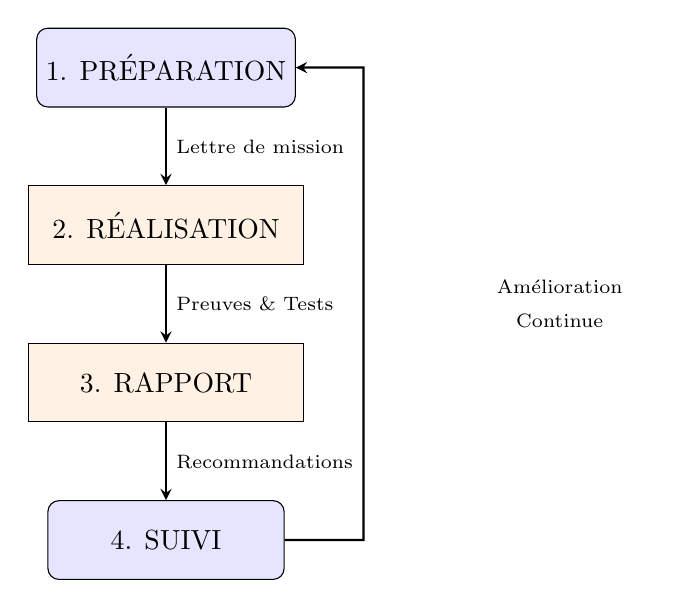
\begin{tikzpicture}[node distance=2cm]
    \tikzstyle{startstop} = [rectangle, rounded corners, minimum width=3cm, minimum height=1cm,text centered, draw=black, fill=blue!10]
    \tikzstyle{process} = [rectangle, minimum width=3.5cm, minimum height=1cm, text centered, draw=black, fill=orange!10]
    \tikzstyle{arrow} = [thick,->,>=stealth]

    \node (p1) [startstop] {1. PRÉPARATION};
    \node (p2) [process, below of=p1] {2. RÉALISATION};
    \node (p3) [process, below of=p2] {3. RAPPORT};
    \node (p4) [startstop, below of=p3] {4. SUIVI};

    \draw [arrow] (p1) -- node[anchor=west] {\scriptsize Lettre de mission} (p2);
    \draw [arrow] (p2) -- node[anchor=west] {\scriptsize Preuves \& Tests} (p3);
    \draw [arrow] (p3) -- node[anchor=west] {\scriptsize Recommandations} (p4);
    
    % Boucle de feedback
    \draw [arrow] (p4.east) -- ++(1,0) -- ++(0,6) -- (p1.east);
    \node at (5,-3) [text width=2.5cm, align=center] {\scriptsize Amélioration Continue};
\end{tikzpicture}
\end{center}


% -------------------------------------------------------------------
% PARTIE II — Référentiels et Typologies d'Audit
% -------------------------------------------------------------------
\part{Référentiels et Typologies d'Audit}

% Chapitre 4 — Normes et référentiels usuels (COSO, COBIT, ISO 27000)
% ==============================================================================
% Fichier : 04_referentiels.tex
% Description : Normes et Référentiels Usuels en Audit des SI
% ==============================================================================

\chapter{Normes et Référentiels Usuels en Audit des Systèmes d'Information}\label{chap:04_referentiels}

L'auditeur a besoin de "briques" techniques et organisationnelles pour évaluer la maturité d'un SI. Les référentiels fournissent les bonnes pratiques reconnues internationalement. Ce chapitre présente les trois piliers : COSO, COBIT et la série ISO 27000.

\section{COSO : Le Modèle de Contrôle Interne}
% ------------------------------------------------------------------------------

\subsection{Présentation}

\begin{boxdef}
\textbf{COSO (Committee of Sponsoring Organizations) :} Cadre de référence conceptuel du contrôle interne, publié en 1992 (révisé en 2013). C'est le modèle standard pour la gouvernance d'entreprise, souvent exigé par les lois sur la gouvernance (ex: Sarbanes-Oxley aux USA).
\end{boxdef}

Bien que généraliste, COSO est le socle sur lequel s'appuient les autres référentiels informatiques.

\subsection{Les Trois Objectifs}

Le contrôle interne selon COSO vise à donner une assurance raisonnable sur la réalisation de trois objectifs :
\begin{enumerate}
    \item \textbf{Réalisation et Optimisation des opérations} (Performance).
    \item \textbf{Fiabilité des informations financières} (Comptabilité).
    \item \textbf{Conformité aux lois et règlements} (Juridique).
\end{enumerate}

\subsection{Les Cinq Composantes (Le Cube COSO)}

Pour atteindre ces objectifs, l'organisation doit mettre en place 5 composantes liées :

\begin{table}[h!]
\centering
\small
\begin{tabular}{p{4cm}p{8cm}}
    \toprule
    \textbf{Composante} & \textbf{Description} \\
    \midrule
    \textbf{Environnement de Contrôle} & La culture, l'éthique, la compétence du personnel. (Le "ton donné par le sommet"). \\
    \textbf{Évaluation des Risques} & Identification et analyse des risques qui pourraient empêcher d'atteindre les objectifs. \\
    \textbf{Activités de Contrôle} & Les politiques et procédures concrètes (Séparation des tâches, autorisations). \\
    \textbf{Information et Communication} & La circulation de l'information nécessaire au pilotage (Qualité des données). \\
    \textbf{Pilotage (Monitoring)} & Surveillance continue du système de contrôle interne (Audits, Supervision). \\
    \bottomrule
\end{tabular}
\caption{Les 5 composantes du référentiel COSO}
\end{table}

\begin{boxlizbiz}
\textbf{Application Lizbiz's :}
L'audit du système de gestion des commandes chez Lizbiz's vérifiera si les 5 composantes COSO sont présentes : existe-t-il une procédure (Activité de contrôle) ? Les risques de fraude sont-ils évalués (Évaluation des risques) ? Les managers supervisent-ils les anomalies (Pilotage) ?
\end{boxlizbiz}

% ------------------------------------------------------------------------------
\section{COBIT : La Gouvernance des SI}
% ------------------------------------------------------------------------------

\subsection{Présentation}

\begin{boxdef}
\textbf{COBIT (Control Objectives for Information and Related Technologies) :} Référentiel de gouvernance et de management des SI développé par l'ISACA. Il fait le pont entre les métiers et l'IT.
\end{boxdef}

C'est le référentiel de choix pour l'auditeur SI car il propose une liste d'objectifs de contrôle précis pour chaque processus informatique.

\subsection{Objectifs et Apports}

COBIT répond à la question : "Comment aligner l'IT sur la stratégie de l'entreprise ?".
Il structure le SI en domaines et processus, offrant à l'auditeur une grille de lecture universelle.

\subsection{Structure de COBIT (Version 5 / 2019)}

COBIT divise la gouvernance et le management en 5 domaines principaux :

\begin{table}[h!]
\centering
\begin{tabular}{lp{10cm}}
    \toprule
    \textbf{Domaine} & \textbf{Contenu (Exemples de processus)} \\
    \midrule
    \textbf{Evaluer, Diriger et Surveiller (EDM)} & Gouvernance stratégique (EDM01 : Gouvernance du cadre IT). \\
    \midrule
    \textbf{Planifier et Organiser (PO)} & Stratégie, Architecture, Budget (PO01 : Gérer le cadre de management IT). \\
    \midrule
    \textbf{Acquérir et Implémenter (AI)} & Projets, Développement, Intégration (AI06 : Gérer les changements). \\
    \midrule
    \textbf{Délivrer et Servir (DS)} & Exploitation, Support, Sécurité (DS01 : Gérer les opérations). \\
    \midrule
    \textbf{Surveiller, Évaluer et Analyser (MEA)} & Performance, Conformité (MEA02 : Surveiller et évaluer le contrôle interne). \\
    \bottomrule
\end{tabular}
\caption{Les domaines de COBIT}
\end{table}

\subsection{Utilisation par l'Auditeur}

Pour chaque processus (ex: DS5 "Gérer la sécurité"), COBIT fournit :
\begin{itemize}
    \item Un objectif de contrôle détaillé.
    \item Des indicateurs de performance (KPI).
    \item Un modèle de maturité (de 0 : Inexistant à 5 : Optimisé).
\end{itemize}

\subsection{La Cascade d'Objectifs COBIT}
L'un des points forts de COBIT est sa capacité à lier la stratégie métier aux objectifs techniques. 
\begin{enumerate}
    \item \textbf{Besoins des parties prenantes} (Bénéfices, Risques, Ressources).
    \item \textbf{Objectifs d'entreprise} (ex: Portefeuille de produits et services structurés).
    \item \textbf{Objectifs d'alignement} (ex: Qualité des informations financières liées à l'IT).
\end{enumerate}
% ------------------------------------------------------------------------------
\section{La Série ISO 27000 : La Sécurité Normative}
% ------------------------------------------------------------------------------

Alors que COBIT gère l'IT, la série ISO 27000 se concentre spécifiquement sur la \textbf{Sécurité de l'Information}.

\subsection{Vue d'Ensemble}

C'est une famille de normes internationales. Les plus critiques pour l'auditeur sont :

\begin{itemize}
    \item \textbf{ISO 27001 :} Exigences pour un Système de Management de la Sécurité de l'Information (SMSI). C'est la norme \textit{certifiable}.
    \item \textbf{ISO 27002 :} Code de bonne pratique. Liste détaillée des mesures de sécurité (contrôles) à implémenter.
    \item \textbf{ISO 27005 :} Gestion des risques en sécurité de l'information.
    \item \textbf{ISO 27006 :} Exigences pour les organismes de certification.
\end{itemize}

\subsection{Importance pour l'Audit}

\begin{enumerate}
    \item \textbf{Critères d'audit :} ISO 27001 fournit les exigences ("Il faut une politique de sécurité"). L'auditeur vérifie si c'est fait.
    \item \textbf{Mesures techniques :} ISO 27002 aide l'auditeur à proposer des recommandations techniques précises (ex: "Comment configurer l'authentification ?").
\end{enumerate}

\begin{boxlizbiz}
\textbf{Projet Lizbiz's :}
Suite à l'audit, la direction de Lizbiz's souhaite rassurer ses clients. Elle décide de se faire certifier \textbf{ISO 27001}. L'auditeur utilisera l'Annexe A de cette norme (qui liste les contrôles obligatoires) comme grille d'évaluation pour le futur audit de certification.
\end{boxlizbiz}

% ------------------------------------------------------------------------------
\section{Synthèse : Comment Choisir ?}
% ------------------------------------------------------------------------------

L'auditeur combine souvent ces référentiels :

\begin{table}[h!]
\centering
\begin{tabular}{p{3cm}p{4cm}p{5cm}}
    \toprule
    \textbf{Référentiel} & \textbf{Angle d'attaque} & \textbf{Question clé pour l'auditeur} \\
    \midrule
    \textbf{COSO} & Gouvernance Globale & Les contrôles internes sont-ils bien conçus ? \\
    \textbf{COBIT} & Processus IT & L'informatique est-elle bien gérée ? \\
    \textbf{ISO 27001} & Sécurité Info & Le système est-il sécurisé et certifiable ? \\
    \bottomrule
\end{tabular}
\caption{Comparatif des référentiels}
\end{table}

\begin{table}[h!]
\centering
\small
\renewcommand{\arraystretch}{1.5}
\begin{tabular}{|l|l|l|l|}
    \hline
    \rowcolor{blue!10} \textbf{Référentiel} & \textbf{Cible} & \textbf{Focus Auditeur} & \textbf{Livrable type} \\ \hline
    \textbf{COSO} & DG / Audit Interne & Contrôle Interne Global & Rapport de conformité Loi Sarbanes-Oxley \\ \hline
    \textbf{COBIT} & DSI / Métiers & Gouvernance et Alignement & Matrice de maturité des processus SI \\ \hline
    \textbf{ISO 27001} & RSSI / Sécurité & Management de la Sécurité & Certification SMSI (Audit de conformité) \\ \hline
\end{tabular}
\caption{Tableau comparatif des référentiels d'audit}
\end{table}


% Chapitre 5 — Principaux types d'audit SI
% ==============================================================================
% Fichier     : 05_types_audits.tex
% Description : Principaux Types d'Audit dans les Systèmes d'Information
% ==============================================================================

\chapter{Principaux Types d'Audit dans les Systèmes d'Information}\label{chap:05_types_audits}

\begin{boxobjectifs}
À l'issue de ce chapitre, l'apprenant doit être capable de :
\begin{itemize}
    \item Distinguer les huit types d'audit SI dans leurs périmètres, enjeux et déclencheurs respectifs ;
    \item Identifier les référentiels internationaux associés à chaque type ;
    \item Comprendre les interactions et dépendances entre types d'audits ;
    \item Positionner chaque type dans le continuum \textit{gouvernance, fonctionnement, sécurité, résilience}.
\end{itemize}
\end{boxobjectifs}

L'audit des systèmes d'information n'est pas un acte monolithique. Il recouvre un spectre de missions dont la nature, le périmètre, les enjeux et la posture de l'auditeur diffèrent profondément selon l'objet examiné. Auditer une application comptable n'appelle pas les mêmes compétences ni les mêmes outils qu'auditer une infrastructure réseau ou un projet en cours de développement. Chaque type d'audit répond à une question fondamentale distincte : \textit{le logiciel fait-il ce qu'on attend de lui ?}, \textit{la DSI est-elle gouvernée efficacement ?}, \textit{le projet sera-t-il livré conformément aux engagements ?}, \textit{le SI résistera-t-il à une cyberattaque ou à un sinistre ?}

Ce chapitre présente les huit grands types d'audit SI rencontrés en milieu professionnel. Pour chacun, la même structure est suivie : enjeu fondamental, périmètre et frontières, fréquence et déclencheurs, dimensions caractéristiques, référentiels mobilisés, interactions avec les autres types et illustration par le cas LiZbiZ. Les décompositions opérationnelles détaillées, points de contrôle, critères, questions d'évaluation, risques et conséquences, font l'objet du chapitre suivant.

\begin{boxinfo}
\textbf{Une lecture systémique.} Les types d'audit ne sont pas étanches. Un audit de la fonction informatique révèle souvent des lacunes dans la gestion des projets ; un audit de sécurité met fréquemment en lumière des déficiences organisationnelles que seul un audit de la DSI aurait pu formellement documenter. L'auditeur SI expérimenté perçoit ces connexions et sait élargir son périmètre lorsque les constats le justifient.
\end{boxinfo}


% ==============================================================================
\section{Audit des Applications en Service}
% ==============================================================================

\subsection{Enjeu fondamental}

Une application en service est un logiciel opérationnel accompagnant, automatisant ou se substituant à un processus de l'organisation, qu'il s'agisse d'un ERP gérant les flux financiers, d'un CRM pilotant la relation client, d'un progiciel de paie ou d'un système de gestion des stocks. Ces applications sont au cœur des processus métiers : leurs défaillances se traduisent directement en pertes financières, en erreurs de traitement ou en violations réglementaires.

L'enjeu de cet audit est double. D'un côté, il s'agit d'émettre une \termecle{assurance raisonnable} sur la fiabilité de l'application, c'est-à-dire sur la qualité de son contrôle interne et la validité des données qu'elle traite et restitue. De l'autre, il s'agit d'apprécier son adéquation aux besoins de l'organisation, sa performance et sa capacité à évoluer avec elle. Ces deux périmètres, fiabilité-sécurité d'une part, efficacité-performance de l'autre, constituent les deux visées distinctes mais complémentaires de l'audit d'application en service. Un audit complet les couvre toutes deux.

\subsection{Périmètre et frontières}

Le périmètre de cet audit couvre l'application elle-même dans toutes ses composantes : programmes, données, paramètres, documentation et habilitations. Il englobe également l'environnement dans lequel elle s'exécute, système d'exploitation, base de données, infrastructure réseau, et les processus organisationnels qui entourent son exploitation : gestion des accès, procédures de sauvegarde, plans de continuité, contrats de maintenance.

La frontière avec l'audit de la fonction informatique mérite d'être précisée. L'audit d'application se concentre sur \textit{ce que fait} le logiciel et \textit{comment il est exploité} ; l'audit de la DSI examine \textit{comment est gouvernée} l'entité qui le produit et le maintient. En pratique, les deux missions se nourrissent mutuellement : une faiblesse détectée dans la gestion des droits d'accès d'une application peut révéler une déficience structurelle dans la politique de sécurité de la DSI.

\subsection{Dimensions caractéristiques}

L'audit d'application en service s'articule autour de deux axes analytiques fondamentaux.

\textbf{Les contrôles généraux} (\textit{General Controls}) couvrent l'environnement global dans lequel l'application fonctionne : sécurité du système d'exploitation hôte, protection physique des serveurs, procédures de sauvegarde et de reprise, gestion des mises à jour et des correctifs, séparation entre les environnements de développement, de test et de production. Ces contrôles conditionnent la fiabilité de tous les contrôles applicatifs : si l'environnement est compromis, aucun contrôle programmatique ne peut être considéré comme fiable.

\textbf{Les contrôles d'application} (\textit{Application Controls}) portent sur le logiciel métier lui-même et s'organisent selon le modèle \termecle{IPO, Input, Process, Output}. En entrée, l'auditeur vérifie que seules des données complètes, exactes et autorisées sont acceptées par le système. En traitement, il s'assure que les calculs et règles de gestion sont correctement implémentés et que les données sensibles sont journalisées. En sortie, il contrôle que les résultats produits sont distribués aux seuls destinataires habilités et que les états de sortie font l'objet d'un contrôle utilisateur effectif.

La \termecle{piste d'audit} (\textit{audit trail}) constitue l'épine dorsale de tout audit d'application : toute action significative sur les données, création, modification, suppression, doit être horodatée, attribuée à un utilisateur identifié et conservée de façon intègre. Son absence est une observation critique majeure.

\subsection{Fréquence et déclencheurs}

La fréquence recommandée est de deux à trois ans pour une application de gestion stable. Mais plusieurs événements doivent déclencher un audit anticipé, indépendamment de ce calendrier : une migration vers une nouvelle version majeure, un changement de prestataire de maintenance, un incident de sécurité impliquant l'application, une évolution réglementaire significative affectant les données traitées, ou encore une croissance rapide du volume de transactions.

\subsection{Référentiels mobilisés}

\norme{COBIT 2019} fournit le cadre de gouvernance ; \norme{ISO/IEC 27034} traite spécifiquement de la sécurité applicative ; \norme{ISO 19011} guide la conduite de la mission d'audit elle-même. Pour les applications financières, les normes \norme{IAS/IFRS} et les exigences de l'auditeur financier externe constituent des référentiels complémentaires incontournables.

\begin{boxlizbiz}
\textbf{LiZbiZ, Pourquoi auditer l'APPLICATION maintenant ?}

LiZbiZ exploite depuis quatre ans un progiciel de gestion commerciale et comptable baptisé \textit{APPLICATION}. Deux signaux ont déclenché la mission : une discordance entre les totaux de la balance comptable et les relevés bancaires sur le trimestre écoulé, et la découverte fortuite par un administrateur qu'un utilisateur avait modifié une facture validée sans qu'aucune trace n'en subsiste dans les logs. Ces deux constats pointent simultanément une défaillance dans les contrôles d'application (absence de piste d'audit sur le module comptable) et une faiblesse dans les contrôles généraux (politique de gestion des droits insuffisante). L'auditeur doit déterminer si la discordance résulte d'une erreur de traitement, d'une manipulation intentionnelle ou d'un bug applicatif.
\end{boxlizbiz}


% ==============================================================================
\section{Audit de la Fonction Informatique (DSI)}
% ==============================================================================

\subsection{Enjeu fondamental}

La Direction des Systèmes d'Information est le pivot organisationnel de toute la chaîne de valeur numérique de l'entreprise. Elle conçoit, déploie, exploite et maintient l'ensemble des actifs informatiques dont dépendent les processus métiers. Auditer la DSI, ce n'est pas auditer une machine ni un logiciel : c'est examiner une \textit{organisation}, sa gouvernance, sa stratégie, ses ressources, ses méthodes, sa culture et son positionnement au sein de l'entreprise.

L'enjeu central est celui de la \termecle{maturité informatique} : la DSI est-elle organisée, dotée, pilotée et régulée de façon à remplir efficacement sa mission et à créer de la valeur pour l'organisation ? Une DSI immature génère des risques en cascade : projets dépassant les délais et les budgets, applications mal maintenues, incidents récurrents non résolus, dépendance critique vis-à-vis de prestataires extérieurs ou de personnes-clés dont le départ pourrait paralyser l'organisation.

\subsection{Périmètre et frontières}

Cet audit couvre six domaines : le rôle et le positionnement de la DSI dans l'organigramme ; sa planification stratégique et l'existence d'un schéma directeur ; la maîtrise de ses budgets et de ses coûts ; la mesure de sa performance ; son organisation interne et la gestion de ses ressources humaines ; enfin, sa conformité au cadre législatif et réglementaire applicable.

La frontière avec l'audit des applications est claire : on s'intéresse ici non pas à ce que produisent les systèmes, mais à la qualité de l'entité qui les produit et les gère. La frontière avec l'audit de sécurité est plus poreuse : la politique de sécurité des SI relève organiquement de la DSI, et sa qualité sera examinée lors des deux types d'audit, sous l'angle organisationnel dans l'audit de la fonction informatique, sous l'angle technique dans l'audit de sécurité.

\subsection{Dimensions caractéristiques}

La \termecle{séparation des tâches} est le premier principe structurant. Elle doit être vérifiée à plusieurs niveaux : entre les équipes de développement et celles de la production, entre l'administration des bases de données et l'exploitation courante, entre la maîtrise d'ouvrage (MOA) et la maîtrise d'œuvre (MOE). Sa violation est un vecteur classique de fraude et d'erreur non détectée.

La \termecle{dépendance aux personnes-clés} est un risque spécifiquement camerounais et africain que l'auditeur doit systématiquement évaluer. Lorsqu'une seule personne détient la connaissance d'un système critique, configuration d'un serveur, paramétrage d'une application, accès à un prestataire —, le départ de cette personne peut paralyser l'organisation. L'auditeur recherche l'existence de procédures documentées, de formations croisées et de plans de succession.

Le \termecle{turn-over} de la DSI constitue un indicateur de santé organisationnelle. Un taux inférieur à 5~\% par an peut signaler une organisation figée ; supérieur à 15~\%, il révèle une instabilité préoccupante susceptible de compromettre la continuité du service.

La conformité au \textbf{cadre législatif camerounais} est un point de contrôle distinctif de ce cours. Les lois de 2010 sur la cybersécurité, la cybercriminalité et les transactions électroniques imposent des obligations précises que la DSI doit connaître et faire respecter. L'auditeur vérifiera que ces textes sont connus des responsables informatiques et que des mesures préventives concrètes ont été mises en place, notamment sur la fraude informatique, le chiffrement, la signature électronique et l'archivage électronique.

\subsection{Fréquence et déclencheurs}

La fréquence recommandée est de trois ans. Les déclencheurs d'un audit anticipé sont : un changement de DSI ou de directeur général, une restructuration organisationnelle majeure, une série d'incidents IT récurrents, ou un audit financier externe ayant relevé des faiblesses dans l'environnement de contrôle informatique.

\subsection{Référentiels mobilisés}

\norme{COBIT 2019} est la référence principale, particulièrement pour les domaines de gouvernance (EDM) et de gestion (APO, BAI, DSS, MEA). \norme{ITIL 4} complète COBIT sur les processus opérationnels. \norme{ISO/IEC 20000-1} traite du management des services informatiques. \norme{ISO 19011} encadre la conduite de la mission.

\begin{boxlizbiz}
\textbf{LiZbiZ, Une DSI sans gouvernance formalisée}

La DSI de LiZbiZ, composée de sept personnes, est dirigée par un responsable informatique qui cumule les fonctions de développeur senior, d'administrateur système et d'interlocuteur contractuel des prestataires. Aucune charte informatique ne définit le périmètre de ses responsabilités. Le schéma directeur date de 2019 et n'a pas été mis à jour depuis la décision d'intégrer l'IA dans la logistique. Le budget IT est intégré au budget général sans ligne de dépense détaillée. Un auditeur n'ayant examiné que l'APPLICATION aurait pu imputer les défaillances constatées à un problème logiciel ; l'audit de la DSI révèle que leur cause racine est organisationnelle.
\end{boxlizbiz}


% ==============================================================================
\section{Audit des Projets Informatiques}
% ==============================================================================

\subsection{Enjeu fondamental}

Les projets informatiques sont des investissements à haut risque. Les études internationales sur l'échec des projets IT, dont le célèbre \textit{Chaos Report} du Standish Group, documentent depuis trente ans que moins de 30~\% des projets IT sont livrés dans les délais, dans les budgets et avec le périmètre fonctionnel initial. Les causes de ces échecs sont rarement techniques : elles sont organisationnelles, méthodologiques et relationnelles.

L'enjeu de l'audit de projet est donc de s'assurer que les mécanismes de pilotage, de qualité et de contrôle sont en place pour maximiser les chances de succès, ou, si le projet est déjà terminé, de documenter les causes d'échec et d'en tirer les enseignements. La question centrale est : \textit{ce projet est-il maîtrisé ?}

\subsection{Périmètre et frontières}

L'audit de projet peut intervenir à deux moments distincts, avec des objectifs différents. L'\textbf{audit de jalons} (\textit{gate review}) intervient en cours de projet, à des étapes prédéfinies, pour vérifier que les conditions de passage à la phase suivante sont réunies. C'est une forme d'audit prospectif : il vise à prévenir les dérives avant qu'elles ne soient irréversibles. L'\textbf{audit de réception} intervient à la clôture du projet pour vérifier la conformité des livrables aux spécifications initiales et tirer les enseignements pour les projets futurs.

Le périmètre couvre l'intégralité du cycle de vie : de l'étude d'opportunité jusqu'à la mise en production et la bascule vers la maintenance. Un projet abandonné ou suspendu doit également faire l'objet d'un audit, pour documenter les causes et éviter que les mêmes erreurs ne se reproduisent.

\subsection{Dimensions caractéristiques}

Le \termecle{triangle QCD}, Qualité, Coût, Délai, est le cadre de référence de l'audit de projet. L'auditeur examine comment ces trois contraintes ont été définies, communiquées, suivies et rééquilibrées au cours du projet. Il est rare qu'un projet respecte simultanément les trois ; la question est de savoir si les arbitrages ont été conscients, documentés et validés par les parties prenantes compétentes.

La distinction entre \termecle{MOA} (Maîtrise d'Ouvrage, le client, définisseur des besoins) et \termecle{MOE} (Maîtrise d'Œuvre, le réalisateur technique) est au cœur de l'audit de projet. L'auditeur vérifie que ces deux rôles sont clairement séparés, que leurs responsabilités sont contractuellement définies et que la MOA a effectivement exercé son rôle de validation à chaque étape, sans se défausser sur la MOE des décisions qui lui appartiennent.

La \termecle{gestion des risques de projet} constitue un point de contrôle critique. L'auditeur recherche l'existence d'un registre des risques, régulièrement mis à jour, avec des plans d'atténuation assignés à des responsables identifiés. L'absence de ce dispositif est un signal d'alarme fort : un projet sans gestion formelle des risques est un projet qui subit les événements au lieu de les anticiper.

\subsection{Fréquence et déclencheurs}

Tout projet doit être audité à son terme. Pour les projets stratégiques ou de grande envergure, des audits de jalons sont recommandés à l'issue de chaque phase majeure. Les signaux déclencheurs d'un audit anticipé non planifié sont : un dépassement budgétaire supérieur à 15~\%, un glissement de planning supérieur à 20~\% du délai initial, un changement de chef de projet, ou des conflits récurrents entre MOA et MOE.

\subsection{Référentiels mobilisés}

\norme{PMBOK} (Project Management Institute) et \norme{PRINCE2} sont les deux référentiels de conduite de projet les plus répandus dans les organisations auditées. \norme{ISO 21500} propose un cadre normatif international harmonisé. Pour les projets agiles, \norme{SCRUM} et \norme{SAFe} constituent les cadres de référence, avec des implications spécifiques sur la façon dont l'auditeur doit adapter sa démarche, les livrables n'étant plus définis ex ante mais émergents.

\begin{boxlizbiz}
\textbf{LiZbiZ, Le projet IA sans garde-fous}

LiZbiZ a lancé il y a huit mois un projet d'intégration d'un algorithme d'apprentissage automatique dans son système de planification logistique. Aucune charte de projet n'a été formalisée. Le budget alloué a déjà été dépassé de 40~\% sans décision formelle de révision. Les données clients utilisées pour entraîner le modèle n'ont fait l'objet d'aucune analyse de conformité RGPD. La MOA, la direction logistique, n'a participé à aucune réunion de validation depuis le lancement. L'audit de jalons déclenché par la direction générale révèle un projet hors de contrôle sur les trois dimensions du triangle QCD, avec un risque juridique réel lié au traitement non conforme des données personnelles.
\end{boxlizbiz}


% ==============================================================================
\section{Audit du Support Utilisateur et de la Gestion du Parc}
% ==============================================================================

\subsection{Enjeu fondamental}

Le support utilisateur et la gestion du parc informatique constituent le visage quotidien de la DSI pour l'ensemble des collaborateurs de l'organisation. La qualité de ce service conditionne directement la productivité des utilisateurs et leur confiance dans les outils informatiques. Un Helpdesk inefficace, des équipements mal inventoriés, des licences non maîtrisées ou des procédures de départ lacunaires sont des risques opérationnels, financiers et de sécurité souvent sous-estimés.

L'enjeu de cet audit est double : évaluer la qualité du service rendu aux utilisateurs, d'une part, et s'assurer de la maîtrise du patrimoine matériel et logiciel de l'organisation, d'autre part. Ces deux objectifs sont liés : on ne peut garantir un bon niveau de service sans connaître précisément les actifs que l'on gère.

\subsection{Dimensions caractéristiques}

La \termecle{gestion des incidents et des demandes} est évaluée à travers l'existence et le suivi des \termecle{SLA} (\textit{Service Level Agreements}) : délai de prise en charge, délai de résolution, taux de résolution au premier contact (\textit{First Call Resolution Rate}). L'auditeur vérifie que ces indicateurs sont effectivement mesurés, communiqués aux utilisateurs et que les écarts font l'objet d'un plan d'amélioration.

La \termecle{procédure d'off-boarding} est un point de contrôle à fort enjeu sécuritaire. Le départ d'un collaborateur, qu'il soit volontaire ou non, doit déclencher immédiatement la révocation de l'ensemble de ses accès logiques (réseau, applications, messagerie, VPN) et la récupération de ses équipements. L'auditeur vérifie l'existence de cette procédure et son effectivité en testant sur un échantillon de départs récents.

\begin{boxlizbiz}
\textbf{LiZbiZ, Le développeur fantôme}

Trois mois après le départ d'un développeur senior, l'auditeur constate que son compte VPN est toujours actif et que ses droits d'accès à l'environnement de production de l'\textit{APPLICATION} n'ont pas été révoqués. Aucune procédure d'off-boarding formalisée n'existe. Le risque est critique : cet ancien collaborateur, qui connaît l'architecture du SI, pourrait se connecter à distance et accéder aux données clients de LiZbiZ sans qu'aucune alerte ne soit générée.
\end{boxlizbiz}


% ==============================================================================
\section{Audit de Sécurité Informatique}
% ==============================================================================

\subsection{Enjeu fondamental}

L'audit de sécurité est le type d'audit SI qui a connu la plus forte croissance au cours des dix dernières années, sous l'effet conjugué de la multiplication des cyberattaques, de la généralisation de la transformation numérique et du durcissement des exigences réglementaires. Son enjeu est de mesurer objectivement la résistance du SI aux menaces, qu'elles soient externes (hackers, groupes criminels organisés, États) ou internes (employés malveillants, erreurs humaines, sous-traitants négligents).

Ce qui distingue fondamentalement l'audit de sécurité des autres types d'audit SI est sa dimension \textit{adversariale} : l'auditeur ne se contente pas de vérifier l'existence de contrôles, il cherche à démontrer leur insuffisance en adoptant la posture d'un attaquant. Les tests d'intrusion (\textit{pentests}) en sont l'expression la plus radicale.

\subsection{Les piliers D.I.C.T.}

L'audit de sécurité s'organise autour des quatre propriétés fondamentales que tout SI doit garantir.

La \termecle{Disponibilité} vise à s'assurer que le système est accessible aux utilisateurs autorisés quand ils en ont besoin, y compris dans des conditions dégradées. Elle est menacée par les pannes matérielles, les saturations de ressources, les attaques par déni de service distribué (DDoS) et les catastrophes naturelles. L'auditeur vérifie l'existence et le test régulier des plans de continuité.

L'\termecle{Intégrité} garantit que les données ne peuvent être modifiées, créées ou supprimées que par des utilisateurs autorisés, selon des processus contrôlés. Sa violation est parfois difficile à détecter : une modification subtile d'un montant dans une base de données comptable peut passer inaperçue pendant des mois si aucun contrôle de cohérence n'est en place.

La \termecle{Confidentialité} assure que l'information n'est accessible qu'aux personnes qui en ont le droit. Elle est menacée par des configurations défectueuses, des droits d'accès excessifs, des données en clair sur des supports non chiffrés ou des communications non sécurisées.

La \termecle{Traçabilité}, parfois appelée imputabilité, garantit que toute action sur le SI peut être attribuée à un acteur identifié et horodatée de façon fiable. Sans elle, il est impossible d'investiguer un incident, de reconstituer une chronologie d'attaque ou d'apporter la preuve d'une fraude devant une juridiction.

\subsection{Dimensions caractéristiques}

L'audit de sécurité mobilise trois méthodologies complémentaires dont la combinaison dépend du périmètre et des objectifs de la mission.

L'\textbf{audit de configuration} consiste à vérifier que les paramètres des systèmes, serveurs, équipements réseau, applications, sont conformes aux référentiels de durcissement (\textit{hardening}) reconnus, tels que les benchmarks \norme{CIS} (\textit{Center for Internet Security}). Il détecte les mots de passe par défaut non modifiés, les services inutiles exposés, les correctifs de sécurité non appliqués.

Les \textbf{tests d'intrusion} (\textit{pentests}) simulent une attaque réelle dans un cadre contractuellement défini, périmètre, règles d'engagement, autorisation écrite préalable obligatoire. Ils peuvent être menés en boîte noire (l'auditeur ne connaît pas l'infrastructure), en boîte grise (il dispose d'informations partielles) ou en boîte blanche (accès complet à la documentation). Le pentest ne remplace pas l'audit de configuration ; il le complète en démontrant l'exploitabilité réelle des vulnérabilités identifiées.

L'\textbf{audit physique} examine la sécurité des locaux : contrôle des accès à la salle des serveurs, gestion des visiteurs, destruction des documents confidentiels, protection contre les sinistres (incendie, inondation, coupure électrique). Il est souvent négligé mais constitue régulièrement le maillon faible de la chaîne de sécurité.

\subsection{Fréquence et déclencheurs}

La fréquence minimale recommandée est annuelle. Les tests de pénétration externes sur les périmètres exposés à Internet, sites web, API, messagerie, VPN, peuvent être plus fréquents, voire continus dans les organisations les plus matures (programme de \textit{bug bounty}). Les déclencheurs d'un audit non planifié sont : tout incident de sécurité significatif, une modification majeure de l'architecture, l'ouverture d'un nouveau périmètre réseau, l'intégration d'un prestataire tiers.

\subsection{Référentiels mobilisés}

\norme{ISO/IEC 27001:2022} est le référentiel de management de la sécurité de l'information, dont l'annexe A liste 93 mesures de sécurité organisées en quatre thèmes. \norme{NIST Cybersecurity Framework v2.0} (2024) propose un cadre fonctionnel articulé autour de six fonctions : Gouverner, Identifier, Protéger, Détecter, Répondre, Rétablir. \norme{ISO/IEC 27035} traite de la gestion des incidents. Pour les tests d'intrusion, le référentiel \norme{PTES} (\textit{Penetration Testing Execution Standard}) et l'environnement \norme{OWASP} pour les applications web font autorité.

\begin{boxlizbiz}
\textbf{LiZbiZ, Trois observations critiques}

Le pentest mené sur le périmètre de LiZbiZ révèle : \textit{(i)} le serveur Apache hébergeant l'\textit{APPLICATION} présente une vulnérabilité critique non corrigée depuis six mois, permettant une exécution de code à distance ; \textit{(ii)} le serveur de base de données comptable est sur le même segment réseau que les postes utilisateurs, supprimant toute barrière entre un poste compromis et les données financières ; \textit{(iii)} les journaux du pare-feu ne sont conservés que sept jours, rendant impossible toute investigation rétrospective sur un incident ayant débuté plusieurs semaines auparavant. Ces trois constats sont interdépendants : un attaquant ayant exploité la vulnérabilité Apache peut latéralement atteindre la base de données sans que personne ne le sache ni ne puisse le prouver.
\end{boxlizbiz}


% ==============================================================================
\section{Audit de la Continuité d'Activité et de la Résilience}
% ==============================================================================

\subsection{Enjeu fondamental}

La résilience organisationnelle désigne la capacité d'une entité à anticiper les disruptions, à y résister et à reprendre ses activités critiques dans des délais compatibles avec sa survie. L'audit de la continuité d'activité ne se demande pas \textit{si} un sinistre surviendra, il postule qu'il surviendra, mais \textit{si l'organisation est prête à y faire face}.

Cet audit est en forte croissance depuis les cyberattaques par rançongiciel (\textit{ransomware}) qui ont paralysé des hôpitaux, des administrations et des entreprises entières, parfois pendant plusieurs semaines. Il est également requis par un nombre croissant de régulateurs sectoriels, banques, assurances, opérateurs d'importance vitale, qui imposent des exigences formelles de continuité.

\subsection{Concepts fondamentaux}

Quatre indicateurs structurent l'évaluation de la résilience.

Le \termecle{BIA} (\textit{Business Impact Analysis}) est le point de départ de tout dispositif de continuité : il identifie les processus critiques de l'organisation, quantifie l'impact d'une interruption sur chacun d'eux et détermine les ressources minimales nécessaires à leur maintien. L'auditeur vérifie l'existence, la complétude et la mise à jour régulière du BIA.

Le \termecle{MTPD} (\textit{Maximum Tolerable Period of Disruption}) est la durée maximale d'interruption d'un processus au-delà de laquelle la survie de l'organisation est menacée. C'est une donnée métier, déterminée par les dirigeants, non par la DSI.

Le \termecle{RTO} (\textit{Recovery Time Objective}) est l'objectif de délai de remise en service des systèmes après un sinistre. Il doit être inférieur au MTPD : un RTO supérieur au MTPD est une incohérence fondamentale que l'auditeur doit impérativement relever.

Le \termecle{RPO} (\textit{Recovery Point Objective}) est la perte de données maximale admissible, exprimée en unité de temps. Il est directement lié à la fréquence des sauvegardes : un RPO de quatre heures implique des sauvegardes au moins toutes les quatre heures.

\begin{boxalert}
\textbf{L'incohérence RTO/RPO : un classique de l'audit.} Un RTO de 4~h avec un RPO de 24~h est techniquement incohérent dans de nombreux contextes : on peut relancer les systèmes en quatre heures, mais avec des données vieilles d'une journée, ce qui peut être inacceptable pour un processus financier ou logistique critique. L'auditeur doit systématiquement vérifier la cohérence de ces paramètres avec les exigences métiers réelles.
\end{boxalert}

\subsection{Fréquence et déclencheurs}

La fréquence recommandée est annuelle, incluant obligatoirement un \textbf{test réel} du Plan de Continuité d'Activité (PCA) et du Plan de Reprise d'Activité (PRA), un plan non testé est un plan dont on ignore s'il fonctionnera. Les déclencheurs d'un audit non planifié sont : tout incident ayant nécessité l'activation du PCA/PRA, une modification significative de l'architecture du SI, ou une nouvelle exigence réglementaire.

\subsection{Référentiels mobilisés}

\norme{ISO 22301:2019} est le standard international du management de la continuité d'activité. \norme{ISO 22317} traite spécifiquement du BIA. \norme{NIST SP 800-34} offre un guide pratique de planification de la continuité pour les systèmes d'information.

\begin{boxlizbiz}
\textbf{LiZbiZ, Un PCA sur papier, jamais testé}

LiZbiZ dispose d'un Plan de Continuité d'Activité rédigé en 2021 par un consultant externe. Ce document identifie correctement les processus critiques et définit un RTO de 4~h et un RPO de 8~h pour l'\textit{APPLICATION}. Cependant, l'auditeur constate : \textit{(i)} le PCA n'a jamais été testé depuis sa rédaction ; \textit{(ii)} les sauvegardes sont effectuées quotidiennement à 23~h, générant un RPO réel de 23~h, incompatible avec l'objectif de 8~h ; \textit{(iii)} les coordonnées de l'hébergeur de secours mentionnées dans le PCA correspondent à un prestataire dont le contrat a été résilié en 2022. Le PCA de LiZbiZ est un document de conformité apparente, pas un dispositif opérationnel.
\end{boxlizbiz}


% ==============================================================================
\section{Audit de la Fonction Étude (Développement)}
% ==============================================================================

\subsection{Enjeu fondamental}

La fonction étude, ou fonction développement, est responsable de la conception, du développement et de la maintenance évolutive des applications de l'organisation. Son audit examine la rigueur des méthodes employées, la qualité du code produit, la maîtrise de la documentation et l'intégration de la sécurité dès la conception. C'est un audit qui requiert à la fois des compétences organisationnelles et une capacité à apprécier la qualité technique des livrables.

L'enjeu principal est de s'assurer que les applications produites en interne, ou développées sous sous-traitance, sont fiables, maintenables, documentées et conformes aux exigences de sécurité. Une fonction étude mal organisée produit une \textit{dette technique} qui s'accumule silencieusement : le code non documenté devient inconnaissable au départ des développeurs qui l'ont écrit, les applications non testées accumulent des bugs latents, les versions non gérées créent des environnements impossibles à reproduire.

\subsection{Dimensions caractéristiques}

La \termecle{séparation des environnements} est un contrôle fondamental : les environnements de développement, de test et de production doivent être strictement séparés. Un développeur ne doit jamais avoir accès direct à la production ; toute mise en production doit passer par une procédure formalisée avec validation indépendante. Sa violation est un facteur de risque majeur, tant pour la fiabilité des applications que pour leur sécurité.

La \termecle{gestion des versions} (\textit{versioning}) assure la traçabilité de l'évolution du code source. L'auditeur vérifie l'utilisation d'un système de contrôle de version (Git ou équivalent), la politique de branches, et la capacité à reproduire un état antérieur du système en cas d'incident.

Le \termecle{Security by Design}, intégration de la sécurité dès la conception, est le paradigme moderne du développement sécurisé. L'auditeur vérifie l'existence de normes de codage sécurisé, la réalisation d'analyses statiques du code (SAST) pour détecter les vulnérabilités classiques (injections SQL, XSS, gestion incorrecte des erreurs) et l'intégration de tests de sécurité dans le pipeline de déploiement (DevSecOps).

\subsection{Fréquence et déclencheurs}

La fréquence recommandée est de deux à trois ans, ou lors de l'adoption d'une nouvelle méthodologie de développement (passage à l'Agile, adoption du DevOps), de l'intégration d'un nouveau prestataire de développement, ou d'un incident applicatif grave ayant pour origine une défaillance du processus de développement.

\subsection{Référentiels mobilisés}

\norme{ISO/IEC 25010} définit les caractéristiques de qualité d'un produit logiciel. \norme{ISO/IEC 27034} traite de la sécurité applicative. \norme{OWASP SAMM} (\textit{Software Assurance Maturity Model}) propose un modèle de maturité pour les pratiques de développement sécurisé. Pour les projets agiles, \norme{SAFe} et les pratiques DevSecOps constituent les références contemporaines.


% ==============================================================================
\section{Audit des Tiers, du Cloud et de l'Externalisation}
% ==============================================================================

\subsection{Enjeu fondamental}

L'externalisation informatique, hébergement cloud, infogérance, sous-traitance de développement, SaaS, transfère des activités et des données à des tiers, mais ne transfère pas la responsabilité. L'organisation reste juridiquement responsable de la sécurité et de la conformité de ses données, y compris lorsqu'elles sont traitées par un prestataire. C'est le principe fondateur du RGPD en matière de sous-traitance : le responsable de traitement doit s'assurer que son sous-traitant offre des garanties suffisantes.

L'audit des tiers répond à une question simple mais dont la réponse est souvent inconfortable : \textit{faites-vous confiance à votre prestataire, ou en avez-vous la preuve ?}

\subsection{Dimensions caractéristiques}

Le \termecle{droit d'audit} est la première vérification contractuelle. Toute convention avec un prestataire hébergeant des données sensibles doit contenir une clause permettant à l'organisation, ou à ses mandataires, d'auditer le prestataire. Son absence prive l'organisation de tout moyen de contrôle indépendant.

Les \termecle{rapports SOC} (\textit{Service Organization Controls}) constituent le substitut standard au droit d'audit direct lorsque celui-ci est contractuellement ou pratiquement impossible, notamment vis-à-vis des grands hyperscalers (AWS, Azure, GCP) qui n'ouvrent pas leurs infrastructures à l'audit individuel de leurs clients. Deux niveaux sont pertinents pour l'auditeur SI :

\begin{itemize}
    \item \textbf{SOC 1 Type II} : évalue les contrôles relatifs au reporting financier sur une période d'observation (généralement six ou douze mois). Pertinent pour les prestataires hébergeant des applications comptables ou financières.
    \item \textbf{SOC 2 Type II} : évalue les contrôles relatifs à la sécurité, la disponibilité, l'intégrité du traitement, la confidentialité et la protection des données personnelles. C'est le rapport le plus fréquemment demandé pour les prestataires cloud hébergeant des données sensibles.
\end{itemize}

L'auditeur ne se contente pas de vérifier l'existence de ces rapports : il en analyse le contenu, notamment les exceptions relevées par l'auditeur du prestataire, et évalue leur pertinence au regard des services effectivement consommés par l'organisation.

La \termecle{cartographie des tiers} est un préalable indispensable à cet audit : l'organisation doit disposer d'un inventaire à jour de tous ses prestataires informatiques, avec pour chacun la nature des données traitées, le niveau de criticité et les mécanismes de contrôle en place.

\subsection{Fréquence et déclencheurs}

La revue des tiers doit être annuelle au minimum. Tout changement significatif chez un prestataire critique, rachat, incident de sécurité public, modification des conditions contractuelles, doit déclencher une revue immédiate.

\subsection{Référentiels mobilisés}

\norme{ISO/IEC 27036} traite spécifiquement de la sécurité des relations avec les fournisseurs. \norme{ISO/IEC 27017} et \norme{27018} complètent ISO 27001 pour les environnements cloud. Le \norme{RGPD} (articles 28 et 29) encadre contractuellement les relations entre responsables de traitement et sous-traitants.

\begin{boxlizbiz}
\textbf{LiZbiZ, Un cloud sans filet}

LiZbiZ héberge ses données clients et ses sauvegardes sur une solution cloud d'un prestataire local. L'auditeur constate : \textit{(i)} le contrat signé ne contient aucune clause d'audit ; \textit{(ii)} le prestataire ne publie aucun rapport SOC et ne dispose d'aucune certification ISO 27001 ; \textit{(iii)} aucun inventaire des prestataires n'existe dans la DSI, le responsable informatique ne peut pas lister de mémoire l'ensemble des services tiers utilisés par l'organisation. LiZbiZ fait confiance à son prestataire sans en avoir la moindre preuve formelle, en violation des obligations qui lui incombent en tant que responsable de traitement de données personnelles.
\end{boxlizbiz}


% ==============================================================================
\section{Interactions entre types d'audit et cartographie du risque SI}
% ==============================================================================

Les huit types d'audit présentés dans ce chapitre ne sont pas des silos indépendants. Ils forment un système d'observation complémentaire dont les résultats se nourrissent mutuellement. Comprendre ces interactions est ce qui distingue l'auditeur expérimenté du technicien compétent.

L'audit de la fonction informatique fournit le cadre organisationnel dans lequel tous les autres audits s'inscrivent : une DSI mal gouvernée génère mécaniquement des faiblesses dans la gestion des applications, des projets et de la sécurité. Il est donc logique de commencer par cet audit lorsqu'une organisation est auditée pour la première fois.

L'audit de sécurité révèle fréquemment des vulnérabilités dont la cause racine est organisationnelle, des droits d'accès excessifs consécutifs à l'absence de procédure d'off-boarding, des correctifs non appliqués faute de processus de gestion des patches, une segmentation réseau déficiente résultant d'une architecture non documentée. Ces causes racines relèvent de l'audit de la fonction informatique, pas de l'audit de sécurité.

L'audit de continuité complète l'audit de sécurité en posant la question \textit{après} l'incident : une fois la cyberattaque survenue, l'organisation est-elle capable de reprendre ses activités ? Les deux audits sont complémentaires et doivent idéalement être conduits de façon coordonnée.

L'audit des tiers conditionne la portée réelle de tous les autres : si les données critiques sont hébergées chez un tiers non audité, les contrôles internes de l'organisation ne valent que pour la fraction du SI qu'elle maîtrise directement.

\begin{boxresume}
\textbf{À retenir.} Les huit types d'audit SI couvrent un continuum allant de la gouvernance (audit de la DSI) au fonctionnement (applications, projets, support) en passant par la sécurité et la résilience (sécurité, continuité) jusqu'à l'écosystème étendu (tiers et cloud). Chaque type répond à une question fondamentale distincte, mobilise des référentiels spécifiques et requiert des compétences particulières. Le chapitre suivant décompose chacun de ces types selon le modèle opérationnel du cours, de la définition du domaine jusqu'à la criticité des conséquences, fournissant ainsi à l'auditeur les instruments de mesure qui transforment ces typologies en missions concrètes.
\end{boxresume}


% -------------------------------------------------------------------
% PARTIE III — Outils d'aide à l'audit
% -------------------------------------------------------------------
\part{Outils d'aide à l'audit}
% Chapitre 6A — 05_theorie_information_shannon
% ==============================================================================
% Fichier  : 05_theorie_information_shannon.tex
% Titre    : Fondements de la Théorie de l'Information de Shannon
%            appliqués à l'Audit des Systèmes d'Information
% Cours    : Audit des Systèmes d'Information – ENSP, Département GI
% Niveau   : Humanités Numériques, Niveau 3
% ==============================================================================

\chapter{Fondements de la Théorie de l'Information de Shannon}
\label{chap:shannon}

% ──────────────────────────────────────────────────────────────────────────────
\section{Pourquoi un auditeur doit-il connaître la théorie de l'information~?}
\label{sec:motivation}
% ──────────────────────────────────────────────────────────────────────────────

L'audit des systèmes d'information est, dans son essence, une activité de
réduction d'incertitude. L'auditeur arrive dans une organisation dont il ignore
l'état réel~: les contrôles sont-ils en place~? La documentation existe-t-elle~?
Les processus sont-ils appliqués~? Chaque question posée, chaque document
examiné, chaque entretien conduit contribue à réduire cette incertitude initiale
et à construire une opinion argumentée sur la qualité du contrôle interne.

Cette réduction progressive de l'incertitude n'est pas seulement une métaphore
intuitive~: elle peut être \emph{mesurée}. C'est précisément l'objet de la
théorie mathématique de l'information, fondée par Claude Elwood Shannon en
1948~\cite{Shannon1948}. Cette théorie fournit une métrique rigoureuse, l'entropie,
qui quantifie l'incertitude contenue dans une distribution de probabilités. Dans
le chapitre suivant, cette métrique sera directement mise en œuvre pour
quantifier l'incertitude résiduelle d'un audit à travers la distribution des
réponses trichotomiques O~/~N~/~PAS. Comprendre son fondement théorique est donc
une condition préalable à l'utilisation correcte et à l'interprétation juste de
l'outil d'aide à l'audit.

Ce chapitre présente les notions fondamentales dans l'ordre de leur construction
logique~: la quantification de l'information (§\,\ref{sec:information}), l'entropie
de Shannon et ses propriétés (§\,\ref{sec:entropie}), la notion d'information
mutuelle et de réduction d'incertitude (§\,\ref{sec:info-mutuelle}), puis
l'application directe à la mesure de l'incertitude dans un audit
(§\,\ref{sec:application-audit}).

\begin{boxlizbiz}
\textbf{Cas Lizbiz's~: l'incertitude comme objet d'audit}

Lors d'une mission préliminaire chez Lizbiz's, l'auditeur senior dresse un bilan
intermédiaire~: sur~30~questions du domaine Sécurité, 10~ont reçu une réponse~O,
10~une réponse~N, et 10~une réponse~PAS. L'équipe dispose donc d'une vision à peu
près aussi informative que le hasard le plus complet. Ce constat, avant même
d'avoir produit un rapport, est \emph{en soi} un constat d'audit~: une
organisation dont les acteurs ne savent pas si ses propres contrôles de sécurité
fonctionnent est une organisation en situation de risque structurel. La mesure
de cette situation par l'entropie de Shannon permettra de la rendre communicable,
comparable et traçable d'un exercice à l'autre.
\end{boxlizbiz}

% ──────────────────────────────────────────────────────────────────────────────
\section{La mesure de l'information}
\label{sec:information}
% ──────────────────────────────────────────────────────────────────────────────

\subsection{Le problème de la surprise}

La question fondatrice de Shannon est d'une simplicité trompeuse~: \emph{combien
d'information apporte un message~?} L'intuition quotidienne suggère que la réponse
dépend du degré de surprise provoqué par ce message. Apprendre que le soleil s'est
levé ce matin n'apporte aucune information~: c'est un événement certain. Apprendre
qu'un système d'information national a subi une intrusion réussie malgré une
politique de sécurité certifiée ISO~27001 est fortement informatif~: c'est un
événement de faible probabilité.

Cette intuition peut être formalisée~: l'information apportée par un événement
doit être une fonction \emph{décroissante} de sa probabilité. Shannon montre
qu'à deux contraintes supplémentaires près, continuité de la fonction et
additivité pour les événements indépendants, il existe une unique famille de
fonctions satisfaisant ces propriétés~\cite{Shannon1948, Cover2006}.

\begin{boxdef}{Information propre (auto-information)}
Soit $\mathcal{X}$ un espace de probabilité fini et $x \in \mathcal{X}$ un
événement de probabilité $p(x) \in (0,\,1]$. L'\emph{information propre}
(ou \emph{auto-information}) de $x$ est définie par~:
\begin{equation}
  I(x) \;=\; -\log_2 p(x) \;\in\; [0,\,+\infty)
  \label{eq:autopinfo}
\end{equation}
L'unité de mesure est le \emph{bit} lorsque le logarithme est en base~2.
\end{boxdef}

Quelques cas limites illustrent la cohérence de cette définition~:
\begin{itemize}
  \item si $p(x) = 1$ (événement certain), alors $I(x) = -\log_2 1 = 0$~: un
        événement certain n'apporte aucune information~;
  \item si $p(x) = 1/2$, alors $I(x) = 1$~bit~: l'issue d'un tirage à pile-ou-face
        équitable apporte exactement~1~bit d'information~;
  \item si $p(x) \to 0$ (événement rarissime), alors $I(x) \to +\infty$~: un événement
        de probabilité quasi nulle serait, s'il se réalisait, porteur d'une
        information quasi infinie.
\end{itemize}

\paragraph{Propriété d'additivité.}
Si $x$ et $y$ sont deux événements \emph{indépendants}, l'information apportée
par leur réalisation conjointe est la somme des informations individuelles~:
\begin{equation}
  I(x,y) \;=\; I(x) + I(y)
  \label{eq:additivite}
\end{equation}
Cette propriété est fondamentale~: elle est la traduction formelle du fait qu'apprendre
deux nouvelles indépendantes est aussi informatif qu'apprendre chacune séparément.

\subsection{De l'événement à la source}

Dans la pratique, on s'intéresse rarement à un événement isolé mais à une
\emph{source d'information}, c'est-à-dire une variable aléatoire $X$ prenant ses
valeurs dans un ensemble fini $\mathcal{X} = \{x_1, \ldots, x_n\}$ avec des
probabilités $p(x_i) = \Pr[X = x_i]$. La question pertinente devient alors~:
quelle est l'incertitude \emph{moyenne} sur la valeur que va prendre $X$, avant
qu'on en connaisse la réalisation~? La réponse est l'entropie de Shannon.

% ──────────────────────────────────────────────────────────────────────────────
\section{L'entropie de Shannon}
\label{sec:entropie}
% ──────────────────────────────────────────────────────────────────────────────

\subsection{Définition}

\begin{boxdef}{Entropie de Shannon}
Soit $X$ une variable aléatoire discrète à valeurs dans $\mathcal{X} =
\{x_1, \ldots, x_n\}$, de loi $p$. L'\emph{entropie de Shannon} de $X$ est la
valeur d'information propre \emph{moyenne} sous la loi $p$~:
\begin{equation}
  H(X) \;=\; \mathbb{E}_{p}\bigl[I(X)\bigr]
           \;=\; -\sum_{i=1}^{n} p(x_i)\,\log_2 p(x_i)
  \label{eq:entropie}
\end{equation}
avec la convention $0 \log_2 0 = 0$ (limite par continuité). L'unité est le
\emph{bit}. $H(X)$ mesure l'incertitude moyenne associée à la source $X$.
\end{boxdef}

La formulation de Shannon est remarquable par sa concision~: elle réduit la notion
d'incertitude, intuitive mais diffuse, à une seule quantité scalaire, calculable,
additive et reliée à la notion de compression optimale de l'information
\cite{Shannon1948, MacKay2003}.

\subsection{Propriétés fondamentales}

Les quatre propriétés suivantes sont des théorèmes démontrables à partir de la
définition~\eqref{eq:entropie}~\cite{Cover2006}.

\begin{boiteTheoreme}{Non-négativité et borne supérieure de l'entropie}
Pour toute variable aléatoire discrète $X$ à $n$ valeurs~:
\begin{equation}
  0 \;\leq\; H(X) \;\leq\; \log_2 n
  \label{eq:bornes}
\end{equation}
\begin{itemize}
  \item $H(X) = 0$ si et seulement si $X$ est \emph{déterministe}~: une et une
        seule valeur $x_i$ a une probabilité~1 (certitude complète, incertitude
        nulle)~;
  \item $H(X) = \log_2 n$ si et seulement si $X$ est \emph{uniformément distribuée}~:
        toutes les valeurs sont équiprobables (incertitude maximale).
\end{itemize}
\end{boiteTheoreme}

\paragraph{Application au contexte trichotomique de l'audit.}
Dans l'outil d'aide à l'audit (chapitre~\ref{chap:06_outil_aide_audit}), les réponses
prennent trois valeurs~: $n = 3$. La borne supérieure de l'entropie est donc
$\log_2 3 \approx 1{,}585$~bits, valeur atteinte lorsque les trois modalités O, N
et PAS/NEK sont équiprobables. C'est le repère cardinal de l'outil~: une entropie
proche de~$1{,}585$ signale que les réponses d'un point de contrôle sont aussi
incertaines que le hasard le plus parfait; une entropie proche de~0 signale une
situation de quasi-certitude (toutes les réponses convergent vers la même
modalité).

\begin{boiteTheoreme}{Concavité de l'entropie}
La fonction $H$ est \emph{strictement concave} sur le simplexe des distributions
de probabilité~: pour toutes distributions $p$ et $q$ et tout $\lambda \in (0,1)$,
\begin{equation}
  H\bigl(\lambda p + (1-\lambda) q\bigr) \;\geq\; \lambda H(p) + (1-\lambda) H(q)
  \label{eq:concavite}
\end{equation}
\end{boiteTheoreme}

La concavité a une interprétation directe~: mélanger deux sources d'information
ne peut qu'augmenter ou conserver l'incertitude, jamais la réduire. En termes
d'audit, agréger les réponses de deux équipes d'auditeurs indépendants sur le même
périmètre ne peut que maintenir ou accroître l'entropie globale~; elle ne saurait
la réduire.

\begin{boiteTheoreme}{Sous-additivité}
Pour deux variables aléatoires $X$ et $Y$, l'entropie jointe satisfait~:
\begin{equation}
  H(X, Y) \;\leq\; H(X) + H(Y)
  \label{eq:sous-additivite}
\end{equation}
avec égalité si et seulement si $X$ et $Y$ sont \emph{indépendantes}.
\end{boiteTheoreme}

\begin{boiteTheoreme}{Entropie conditionnelle et règle de chaînage}
L'\emph{entropie conditionnelle} de $X$ sachant $Y$ est l'incertitude résiduelle
sur $X$ lorsque $Y$ est connue~:
\begin{equation}
  H(X \mid Y) \;=\; -\sum_{j} p(y_j) \sum_{i} p(x_i \mid y_j)\,\log_2 p(x_i \mid y_j)
  \label{eq:entropie-cond}
\end{equation}
La \emph{règle de chaînage} s'écrit alors~:
\begin{equation}
  H(X, Y) \;=\; H(X) + H(Y \mid X) \;=\; H(Y) + H(X \mid Y)
  \label{eq:chainage}
\end{equation}
On a toujours $H(X \mid Y) \leq H(X)$~: la connaissance d'une observation $Y$
ne peut qu'égaler ou réduire l'incertitude sur $X$, jamais l'augmenter.
\end{boiteTheoreme}

\subsection{Illustration sur des distributions élémentaires}

Le tableau~\ref{tab:entropies} calcule l'entropie pour plusieurs distributions
trichotomiques représentatives de situations d'audit.

\begin{table}[H]
\centering
\small
\caption{Entropie de Shannon pour des distributions trichotomiques {O, N, PAS}
représentatives de situations d'audit}
\label{tab:entropies}
\begin{tabular}{lccccc}
\toprule
\textbf{Situation d'audit} & $p_O$ & $p_N$ & $p_P$ &
$H$ (bits) & \textbf{Interprétation} \\
\midrule
Conformité totale &
1{,}00 & 0{,}00 & 0{,}00 & 0{,}000 & Certitude~: aucune zone d'ombre \\
\addlinespace
Forte non-conformité &
0{,}10 & 0{,}80 & 0{,}10 & 0{,}922 & Situation dégradée mais lisible \\
\addlinespace
Forte incertitude &
0{,}10 & 0{,}10 & 0{,}80 & 0{,}922 & Carence informationnelle majeure \\
\addlinespace
Incertitude modérée &
0{,}50 & 0{,}25 & 0{,}25 & 1{,}500 & Zone grise significative \\
\addlinespace
Incertitude maximale &
$\frac{1}{3}$ & $\frac{1}{3}$ & $\frac{1}{3}$ & 1{,}585 & Chaos informationnel \\
\bottomrule
\end{tabular}
\end{table}

Deux observations méritent d'être soulignées. Premièrement, une forte
non-conformité avérée (distribution $0{,}10$-$0{,}80$-$0{,}10$) et une forte
carence documentaire (distribution $0{,}10$-$0{,}10$-$0{,}80$) produisent la
\emph{même} entropie~: les deux situations sont, du point de vue informationnel,
également certaines, bien qu'elles appellent des recommandations distinctes.
Deuxièmement, la situation de zone grise modérée ($0{,}50$-$0{,}25$-$0{,}25$),
qui pourrait paraître rassurante du fait de la majorité de réponses O, est
presque aussi entropique que le désordre complet~: la présence de~$25\,\%$ de
réponses PAS/NEK suffit à élever fortement l'incertitude globale.

\begin{boiteRemarque}{Calcul de l'entropie~: règle de convention}
Par définition, $0 \log_2 0 = 0$. Cette convention est indispensable pour que
la formule~\eqref{eq:entropie} reste valide lorsqu'une ou plusieurs modalités
ont une probabilité nulle. Dans un tableur, elle se traduit par l'usage d'un
test conditionnel~: \verb|SI(p=0;0;p*LOG(p;2))|. Omettre cette convention produit
une erreur de division par zéro.
\end{boiteRemarque}

% ──────────────────────────────────────────────────────────────────────────────
\section{Information mutuelle et réduction d'incertitude}
\label{sec:info-mutuelle}
% ──────────────────────────────────────────────────────────────────────────────

\subsection{Définition}

La notion d'information mutuelle formalise la question~: \emph{combien une
observation $Y$ réduit-elle l'incertitude sur $X$~?} C'est la traduction
quantitative de l'activité même de l'audit.

\begin{boxdef}{Information mutuelle}
L'\emph{information mutuelle} de deux variables aléatoires $X$ et $Y$ est
définie par~:
\begin{equation}
  I(X\,;\,Y) \;=\; H(X) - H(X \mid Y) \;=\; H(Y) - H(Y \mid X)
  \label{eq:info-mutuelle}
\end{equation}
Elle mesure la réduction d'incertitude sur $X$ apportée par la connaissance de
$Y$, et réciproquement. On a $I(X\,;\,Y) \geq 0$, avec égalité si et seulement
si $X$ et $Y$ sont indépendantes.
\end{boxdef}

L'information mutuelle s'exprime également comme la divergence de
Kullback-Leibler~\cite{Kullback1951} entre la loi jointe $p(x,y)$ et le produit
des lois marginales $p(x)\,p(y)$~:
\begin{equation}
  I(X\,;\,Y) \;=\; \sum_{x,y} p(x,y)\,\log_2 \frac{p(x,y)}{p(x)\,p(y)}
  \label{eq:kl}
\end{equation}

\subsection{Interprétation dans le contexte de l'audit}

La table~\ref{tab:analogie-audit} établit le parallèle entre les notions de la
théorie de l'information et les réalités de la mission d'audit.

\begin{table}[H]
\centering
\small
\caption{Correspondance entre théorie de l'information et pratique de l'audit}
\label{tab:analogie-audit}
\begin{tabular}{p{4.5cm}p{4.5cm}p{4.5cm}}
\toprule
\textbf{Notion formelle} & \textbf{Notation} & \textbf{Réalité de l'audit} \\
\midrule
Variable aléatoire $X$ &
$X$ : état réel du contrôle &
Le contrôle est-il effectif~? L'auditeur l'ignore avant l'audit. \\
\addlinespace
Distribution a priori de $X$ &
$p(x)$ avant investigation &
Croyances initiales de l'auditeur~; en l'absence de données~: 
distribution uniforme sur O/N/PAS. \\
\addlinespace
Observation $Y$ &
Réponse obtenue (O, N, PAS) &
Réponse à une question d'évaluation, document examiné, entretien conduit. \\
\addlinespace
Entropie a priori $H(X)$ &
Incertitude avant investigation &
Incertitude totale à l'ouverture de la mission. \\
\addlinespace
Entropie a posteriori $H(X \mid Y)$ &
Incertitude après observation &
Incertitude résiduelle après collecte des preuves. \\
\addlinespace
Information mutuelle $I(X\,;\,Y)$ &
$H(X) - H(X \mid Y)$ &
Valeur informative d'une question d'audit~: réduction d'incertitude produite
par l'investigation. \\
\bottomrule
\end{tabular}
\end{table}

La mission d'audit peut donc se lire comme un processus de maximisation de
l'information mutuelle~: l'auditeur cherche, par son plan d'investigation, à
maximiser $I(X\,;\,Y_1, \ldots, Y_k)$, c'est-à-dire à sélectionner les questions
et les observations qui réduisent le plus l'incertitude initiale $H(X)$. Un
point de contrôle pour lequel l'entropie reste élevée après investigation, parce
que toutes les réponses sont PAS/NEK, est un point pour lequel l'information
mutuelle entre les observations et l'état réel du contrôle est nulle~: les
questions posées n'ont apporté aucune réduction d'incertitude. C'est un constat
d'audit en soi.

\subsection{La divergence de Kullback-Leibler et la mesure de l'écart normatif}

La théorie de l'information offre un outil complémentaire~: la divergence de
Kullback-Leibler (KL), qui mesure l'écart entre une distribution observée et une
distribution de référence~\cite{Kullback1951}.

\begin{boxdef}{Divergence de Kullback-Leibler}
Soient $p$ (distribution observée) et $q$ (distribution de référence) deux
distributions sur un espace fini $\mathcal{X}$. La \emph{divergence KL} de $p$
par rapport à $q$ est~:
\begin{equation}
  D_{\mathrm{KL}}(p \,\|\, q) \;=\; \sum_{x \in \mathcal{X}} p(x)\,\log_2\frac{p(x)}{q(x)}
  \label{eq:kl-div}
\end{equation}
avec $D_{\mathrm{KL}}(p \,\|\, q) \geq 0$ et égalité si et seulement si $p = q$
(inégalité de Gibbs~\cite{Cover2006}).
\end{boxdef}

Dans le contexte de l'audit, $q$ peut représenter la distribution cible d'une
organisation mature, par exemple $q = (0{,}90,\,0{,}05,\,0{,}05)$ pour
un domaine bien contrôlé, et $p$ la distribution observée lors d'une mission.
La divergence KL mesure alors l'écart entre la réalité observée et l'état
souhaité~: c'est un indicateur synthétique de la distance entre la maturité
effective et la maturité cible.

\begin{boiteRemarque}{Non-symétrie de la divergence KL}
La divergence KL n'est pas symétrique~: $D_{\mathrm{KL}}(p \,\|\, q) \neq
D_{\mathrm{KL}}(q \,\|\, p)$ en général. Elle ne définit donc pas une distance
au sens mathématique strict. Pour des usages où la symétrie est souhaitable
(comparaison entre deux unités auditées), on lui préfère la divergence de Jensen-Shannon,
définie comme la moyenne des divergences KL de $p$ et $q$ vers leur mélange
$m = \frac{1}{2}(p+q)$~\cite{Lin1991}. Son usage reste optionnel dans le cadre de
ce cours~; la divergence KL suffit pour les applications présentées au chapitre
suivant.
\end{boiteRemarque}

% ──────────────────────────────────────────────────────────────────────────────
\section{Le codage de l'information~: lien avec la compression}
\label{sec:codage}
% ──────────────────────────────────────────────────────────────────────────────

L'entropie possède une interprétation opérationnelle fondamentale qui en justifie
le nom et en éclaire le sens profond~: elle représente la \emph{longueur minimale
moyenne} d'un code nécessaire pour représenter les messages d'une source. Ce
résultat est le \emph{théorème du codage source} de Shannon.

\begin{boiteTheoreme}{Théorème du codage source (Shannon, 1948)}
Soit $X$ une source discrète sans mémoire de loi $p$. Tout code préfixe
(code de Huffman~\cite{Huffman1952}, par exemple) attribue à chaque symbole $x_i$
un mot de code de longueur $\ell_i$. La \emph{longueur moyenne} $\bar{L} =
\sum_i p(x_i)\,\ell_i$ satisfait~:
\begin{equation}
  H(X) \;\leq\; \bar{L} \;<\; H(X) + 1
  \label{eq:codage-source}
\end{equation}
La borne inférieure $H(X)$ est atteinte asymptotiquement~: l'entropie est la
limite fondamentale de la compression sans perte.
\end{boiteTheoreme}

L'interprétation pour l'audit est la suivante. Si un point de contrôle présente
une entropie $H \approx 0$, ses réponses sont quasi certaines~: elles sont peu
informatives dans l'absolu, mais elles sont \emph{compressibles} en très peu de
bits. À l'inverse, une entropie $H \approx 1{,}585$~bits signifie que les
réponses de ce point de contrôle sont si imprévisibles qu'elles nécessitent la
quasi-totalité du potentiel informationnel d'un système à trois symboles~: chaque
réponse est véritablement une \emph{nouvelle} au sens informationnel du terme.

Cette intuition rejoint directement la pratique de l'audit~: un point de contrôle
à forte entropie mérite plus de temps, d'investigations complémentaires et de
diligences documentaires, précisément parce que chaque réponse y est plus
susceptible d'être surprenante et donc potentiellement révélatrice.

% ──────────────────────────────────────────────────────────────────────────────
\section{Entropie et distributions trichotomiques~: analyse exhaustive}
\label{sec:trichotomique}
% ──────────────────────────────────────────────────────────────────────────────

\subsection{Paramétrisation de la surface d'entropie}

La surface d'entropie d'une distribution trichotomique $(p_O, p_N, p_P)$ avec
$p_O + p_N + p_P = 1$ forme un simplexe bidimensionnel. Son étude complète
permet de comprendre comment chacun des trois types de réponse contribue à l'entropie
globale.

En posant $\mathbf{p} = (p_O, p_N, p_P)$, on a~:
\begin{equation}
  H(\mathbf{p})
    = -p_O \log_2 p_O - p_N \log_2 p_N - p_P \log_2 p_P
    \;\in\; [0,\; \log_2 3]
  \label{eq:entropie-tri}
\end{equation}

Les lignes de niveau de cette surface révèlent trois zones de qualité distinctes~:

\begin{enumerate}
  \item \textbf{Zone de certitude} ($H < 0{,}5$~bit)~: au moins l'une des trois
        modalités est largement dominante. L'audit est conclusif, même si la
        conclusion est défavorable. Un audit entièrement rouge (toutes les
        réponses~N) est, paradoxalement, aussi informatif qu'un audit entièrement
        vert~: dans les deux cas, $H = 0$.
  \item \textbf{Zone d'incertitude modérée} ($0{,}5 \leq H < 1{,}0$~bit)~:
        les réponses sont partagées mais avec une tendance perceptible.
        L'investigation complémentaire est utile mais non urgente.
  \item \textbf{Zone grise critique} ($H \geq 1{,}0$~bit)~: les trois modalités
        coexistent de façon significative. L'audit de ce point de contrôle doit
        être étendu avant que toute conclusion soit émise.
\end{enumerate}

\subsection{Décomposition de l'entropie et contribution des composantes}

L'entropie d'une distribution trichotomique peut se décomposer en la somme de
l'entropie binaire O~vs.~(N+PAS) et de l'entropie conditionnelle sur la
répartition N/PAS~:
\begin{equation}
  H(p_O, p_N, p_P) \;=\;
    H_b(p_O) \;+\; (1 - p_O)\,H\!\left(\frac{p_N}{1-p_O},\;
    \frac{p_P}{1-p_O}\right)
  \label{eq:decomp}
\end{equation}
où $H_b(\alpha) = -\alpha \log_2 \alpha - (1-\alpha)\log_2(1-\alpha)$ est
l'entropie binaire de Bernoulli. Cette décomposition est utile pour identifier
la source principale d'incertitude~: le premier terme mesure l'incertitude sur la
dichotomie conformité/non-conformité, tandis que le second mesure l'incertitude
entre non-conformité avérée et incertitude documentaire.

% ──────────────────────────────────────────────────────────────────────────────
\section{Application à la mesure de l'incertitude dans un audit}
\label{sec:application-audit}
% ──────────────────────────────────────────────────────────────────────────────

\subsection{Modélisation formelle du processus d'audit}

Soit $\mathcal{D}$ un domaine d'audit décomposé en $K$ points de contrôle
$\{C_1, \ldots, C_K\}$, et soit $C_k$ un point de contrôle comportant $n_k$
questions d'évaluation. Pour chaque question $j \in \{1, \ldots, n_k\}$, l'auditeur
collecte une réponse $r_{k,j} \in \{\texttt{O},\,\texttt{N},\,\texttt{PAS}\}$.

\begin{boxdef}{Entropie d'un point de contrôle}
Notons $n_k^O$, $n_k^N$, $n_k^P$ les effectifs de chaque modalité dans le point
de contrôle $C_k$, et $n_k = n_k^O + n_k^N + n_k^P$ le nombre total de questions.
L'\emph{entropie empirique} du point de contrôle est~:
\begin{equation}
  H(C_k) \;=\; -\!\!\!\sum_{m \,\in\, \{\texttt{O},\texttt{N},\texttt{P}\}}
  \hat{p}_{k,m}\,\log_2 \hat{p}_{k,m}
  \label{eq:entropie-cp}
\end{equation}
où $\hat{p}_{k,m} = n_k^m / n_k$ est la fréquence observée de la modalité~$m$.
\end{boxdef}

\begin{boxdef}{Entropie d'un domaine (entropie agrégée)}
L'\emph{entropie du domaine} $\mathcal{D}$ est la moyenne pondérée des entropies
de ses points de contrôle, pondérée par le nombre de questions~:
\begin{equation}
  H(\mathcal{D}) \;=\; \frac{\displaystyle\sum_{k=1}^{K} n_k\,H(C_k)}{\displaystyle\sum_{k=1}^{K} n_k}
  \label{eq:entropie-domaine}
\end{equation}
Cette quantité est l'entropie empirique calculée sur l'ensemble des réponses du
domaine, traitées comme un seul échantillon.
\end{boxdef}

\subsection{Le double signal de l'outil d'audit}

Le chapitre~\ref{chap:06_outil_aide_audit} introduit l'idée que l'outil mesure deux
dimensions distinctes~: \emph{ce qui ne va pas} (taux de non-conformité,
proportion de réponses~N) et \emph{ce qu'on ne sait pas} (proportion de réponses
PAS/NEK). La théorie de Shannon éclaire pourquoi ces deux dimensions sont
fondamentalement irréductibles l'une à l'autre.

Formellement, les deux signaux sont~:
\begin{align}
  \tau_c(\mathcal{D}) &= \hat{p}_O \;=\; \frac{n^O}{n}
  \label{eq:taux-conformite} \\[6pt]
  H(\mathcal{D}) &= -\hat{p}_O \log_2 \hat{p}_O
                   - \hat{p}_N \log_2 \hat{p}_N
                   - \hat{p}_P \log_2 \hat{p}_P
  \label{eq:entropie-domaine2}
\end{align}

Ces deux indicateurs sont \emph{orthogonaux}~: deux domaines de même taux de
conformité peuvent présenter des entropies très différentes, et inversement. Le
tableau~\ref{tab:ortho} illustre cette orthogonalité.

\begin{table}[H]
\centering
\small
\caption{Orthogonalité du taux de conformité et de l'entropie~: quatre
configurations distinctes pour un même taux de conformité de~$50\,\%$}
\label{tab:ortho}
\begin{tabular}{lccccc}
\toprule
\textbf{Configuration} & $\hat{p}_O$ & $\hat{p}_N$ & $\hat{p}_P$ &
$\tau_c$ & $H$ (bits) \\
\midrule
Audit clair, moitié conforme & 0{,}50 & 0{,}50 & 0{,}00 & 50\,\% & 1{,}000 \\
Audit ambigu, sans zone grise & 0{,}50 & 0{,}25 & 0{,}25 & 50\,\% & 1{,}500 \\
Forte carence documentaire & 0{,}50 & 0{,}10 & 0{,}40 & 50\,\% & 1{,}361 \\
Incertitude maximale & $\frac{1}{3}$ & $\frac{1}{3}$ & $\frac{1}{3}$ & 33\,\% & 1{,}585 \\
\bottomrule
\end{tabular}
\end{table}

Ces quatre situations n'ont pas le même profil de risque, bien que les deux
premières partagent le même taux de conformité de~$50\,\%$. Dans la première,
l'auditeur sait ce qui va et ce qui ne va pas~; dans la seconde, un quart des
réponses reste dans la zone grise, ce qui signifie qu'un quart du périmètre
audité est soustrait à l'opinion de l'auditeur. Réduire l'audit à son seul taux
de conformité reviendrait à traiter ces situations de façon identique, ce qui
serait une erreur méthodologique grave.

\subsection{Interprétation normative des seuils d'entropie}

La table~\ref{tab:seuils} résume les seuils d'interprétation de l'entropie en
contexte d'audit, tels qu'ils seront mis en œuvre dans l'outil du chapitre
suivant.

\begin{table}[H]
\centering
\small
\caption{Seuils normatifs d'entropie pour l'interprétation d'un point de
contrôle dans l'outil d'aide à l'audit} 
\label{tab:seuils}
\begin{tabular}{cccl}
\toprule
\textbf{Plage} & \textbf{Couleur outil} & \textbf{Qualification} &
\textbf{Conduite à tenir} \\
\midrule
$H < 0{,}5$ & Blanc & Certitude & Aucune investigation complémentaire requise \\
$0{,}5 \leq H < 1{,}0$ & Jaune & Incertitude modérée &
Relance de l'audité sur les PAS/NEK \\
$H \geq 1{,}0$ & Rouge & Zone grise critique &
Investigation approfondie obligatoire avant conclusion \\
\bottomrule
\end{tabular}
\end{table}

\begin{boiteRemarque}{Nature statistique de l'entropie empirique}
L'entropie~$H(C_k)$ calculée dans l'outil est une \emph{entropie empirique}~:
elle est estimée sur un échantillon fini de $n_k$ questions. Pour des points de
contrôle comportant peu de questions ($n_k < 10$), l'estimation peut être biaisée
et instable. L'estimateur du maximum de vraisemblance de l'entropie est
asymptotiquement non biaisé mais surestimé pour de petits $n$~\cite{Paninski2003}.
Des correcteurs de biais (correcteur de Miller-Madow) existent mais ne sont pas
nécessaires dans le cadre de ce cours, où l'entropie est utilisée comme indicateur
de pilotage et non comme estimateur statistique précis.
\end{boiteRemarque}

% ──────────────────────────────────────────────────────────────────────────────
\section{Extensions~: entropie croisée et mesures apparentées}
\label{sec:extensions}
% ──────────────────────────────────────────────────────────────────────────────

Pour les lecteurs souhaitant aller plus loin, deux extensions de la notion
d'entropie de Shannon sont présentées~: l'entropie croisée, utilisée pour mesurer
l'adéquation d'un modèle à une distribution observée, et l'entropie de Rényi,
qui généralise l'entropie de Shannon à une famille paramétrée.

\begin{boxdef}{Entropie croisée}
Soient $p$ (distribution réelle) et $q$ (distribution modèle) deux distributions
sur $\mathcal{X}$. L'\emph{entropie croisée} de $p$ relativement à $q$ est~:
\begin{equation}
  H(p, q) \;=\; -\sum_{x \in \mathcal{X}} p(x)\,\log_2 q(x)
  \label{eq:entropie-croisee}
\end{equation}
On a $H(p,q) = H(p) + D_{\mathrm{KL}}(p\,\|\,q) \geq H(p)$, avec égalité si
et seulement si $p = q$.
\end{boxdef}

En audit, $q$ peut représenter la distribution cible d'une organisation certifiée
(ex.~$q_{\mathrm{cible}} = (0{,}90, 0{,}05, 0{,}05)$) et $p$ la distribution observée.
L'entropie croisée $H(p, q_{\mathrm{cible}})$ mesure alors le coût informationnel
de l'inadéquation entre la réalité et la cible~: plus ce coût est élevé, plus
l'organisation s'écarte de son niveau de maturité attendu.

\begin{boxdef}{Entropie de Rényi}
Soit $\alpha > 0$, $\alpha \neq 1$. L'\emph{entropie de Rényi d'ordre $\alpha$}
est~:
\begin{equation}
  H_\alpha(X) \;=\; \frac{1}{1-\alpha}\,\log_2\!\left(\sum_{i} p(x_i)^\alpha\right)
  \label{eq:renyi}
\end{equation}
À la limite $\alpha \to 1$, $H_\alpha(X) \to H(X)$ (entropie de Shannon).
\end{boxdef}

L'entropie de Rényi d'ordre~$\alpha > 1$ pénalise davantage les événements
fréquents et est moins sensible aux événements rares~; pour $\alpha < 1$,
l'effet inverse se produit. Dans le contexte de l'audit, l'entropie de Rényi
d'ordre~2 ($H_2$), appelée \emph{entropie de collision}, offre une mesure
d'incertitude plus robuste aux petites erreurs d'estimation des probabilités~;
elle peut être utilisée comme vérification de la stabilité des résultats obtenus
avec l'entropie de Shannon standard~\cite{Renyi1961}.

% ──────────────────────────────────────────────────────────────────────────────
\section{Synthèse~: de Shannon à l'audit}
\label{sec:synthese}
% ──────────────────────────────────────────────────────────────────────────────

Ce chapitre a construit le socle théorique nécessaire à la pleine compréhension
de l'outil d'aide à l'audit présenté au chapitre suivant. La progression logique
en est la suivante~:

\begin{enumerate}
  \item L'information propre $I(x) = -\log_2 p(x)$ quantifie la surprise associée
        à l'observation d'un événement isolé~; son analogue en audit est l'apport
        informationnel d'une seule réponse d'évaluation.
  \item L'entropie de Shannon $H(X)$ est la moyenne de cette surprise sur
        l'ensemble d'une source~; appliquée à un point de contrôle, elle mesure
        l'incertitude résiduelle de l'auditeur après investigation.
  \item L'information mutuelle $I(X\,;\,Y)$ mesure la réduction d'incertitude
        apportée par une observation~; elle formalise la valeur informative d'un
        programme d'audit~: un bon plan d'audit est celui qui maximise la
        réduction d'incertitude pour un coût d'investigation donné.
  \item Le théorème du codage source relie l'entropie à la compressibilité~;
        un point de contrôle à entropie élevée est, au sens formel, un point
        dont les réponses sont fondamentalement incompressibles~: elles ne peuvent
        être prédites ni remplacées par des connaissances préalables.
  \item La divergence de Kullback-Leibler permet de mesurer l'écart entre l'état
        observé d'un domaine et un référentiel de maturité cible~; elle est
        l'instrument formel de la notation de maturité.
\end{enumerate}

\begin{boiteTheoreme}{Principe de la cartographie entropique en audit}
Soit un audit portant sur $K$ points de contrôle. Définissons le vecteur
d'entropies $\mathbf{H} = (H(C_1), \ldots, H(C_K)) \in [0,\,\log_2 3]^K$.
La \emph{cartographie entropique} de l'audit est la représentation graphique de
$\mathbf{H}$. Elle constitue un second tableau de bord orthogonal au vecteur des
taux de conformité $\boldsymbol{\tau} = (\tau_{c,1}, \ldots, \tau_{c,K})$.

Les quatre quadrants du plan $(\tau_c, H)$ correspondent à quatre pathologies
distinctes~:
\begin{itemize}
  \item $(\tau_c$ élevé, $H$ faible)~: bonne conformité, haute lisibilité~---
        la situation nominale visée~;
  \item $(\tau_c$ faible, $H$ faible)~: non-conformité massive mais clairement
        identifiée, situation grave mais traçable~;
  \item $(\tau_c$ élevé, $H$ élevée)~: apparence de conformité masquée par une
        carence d'information, situation trompeuse, à risque sous-estimé~;
  \item $(\tau_c$ faible, $H$ élevée)~: non-conformité probable et incertitude
        élevée, la situation la plus préoccupante, requérant une investigation
        immédiate.
\end{itemize}
\end{boiteTheoreme}

\begin{boxlizbiz}
\textbf{Cas Lizbiz's~: lecture de la cartographie entropique}

À l'issue de l'audit de Lizbiz's, la feuille \texttt{SYNTHÈSE} produit le
vecteur d'entropies suivant pour cinq domaines~:

\smallskip
\begin{tabular}{lccl}
\toprule
\textbf{Domaine} & $\tau_c$ & $H$ (bits) & \textbf{Quadrant} \\
\midrule
Applications & $78\,\%$ & $0{,}62$ & Bonne conformité, lisibilité moyenne \\
DSI & $55\,\%$ & $0{,}38$ & Non-conformité marquée, lisible \\
Projets & $82\,\%$ & $1{,}21$ & \textbf{Conformité apparente, fort risque masqué} \\
Support & $91\,\%$ & $0{,}18$ & Situation nominale \\
Sécurité & $33\,\%$ & $1{,}40$ & \textbf{Non-conformité et incertitude critiques} \\
\bottomrule
\end{tabular}

\smallskip
La lecture du seul taux de conformité aurait conduit à concentrer les
recommandations sur les domaines DSI et Sécurité. La cartographie entropique
révèle que le domaine Projets, apparemment sain ($\tau_c = 82\,\%$), est en
réalité une zone grise critique ($H = 1{,}21$~bits)~: plus de la moitié des
réponses de ce domaine sont PAS/NEK, signalant une organisation de projet dont
personne ne connaît le fonctionnement réel. Ce domaine exige une investigation
complémentaire prioritaire avant que l'auditeur puisse émettre une opinion.
\end{boxlizbiz}

% ──────────────────────────────────────────────────────────────────────────────
\section*{Références bibliographiques}
% ──────────────────────────────────────────────────────────────────────────────

\addcontentsline{toc}{section}{Références bibliographiques}

\begin{itemize}

\item \textsc{Shannon}, C.\,E. (1948). A mathematical theory of communication.
\emph{Bell System Technical Journal}, 27(3), 379--423 \& 27(4), 623--656.
\href{https://doi.org/10.1002/j.1538-7305.1948.tb01338.x}{DOI}

\item \textsc{Cover}, T.\,M. et \textsc{Thomas}, J.\,A. (2006).
\emph{Elements of Information Theory} (2\textsuperscript{e}~éd.).
Wiley-Interscience. ISBN 978-0-471-24195-9.

\item \textsc{MacKay}, D.\,J.\,C. (2003).
\emph{Information Theory, Inference, and Learning Algorithms}.
Cambridge University Press. ISBN 978-0-521-64298-9.
Disponible en libre accès~: \url{http://www.inference.org.uk/mackay/itila/}

\item \textsc{Kullback}, S. et \textsc{Leibler}, R.\,A. (1951).
On information and sufficiency.
\emph{The Annals of Mathematical Statistics}, 22(1), 79--86.
\href{https://doi.org/10.1214/aoms/1177729694}{DOI: 10.1214/aoms/1177729694}

\item \textsc{Huffman}, D.\,A. (1952).
A method for the construction of minimum-redundancy codes.
\emph{Proceedings of the IRE}, 40(9), 1098--1101.
\href{https://doi.org/10.1109/JRPROC.1952.273898}{DOI: 10.1109/JRPROC.1952.273898}
\item \textsc{Lin}, J. (1991).
Divergence measures based on the Shannon entropy.
\emph{IEEE Transactions on Information Theory}, 37(1), 145--151.
\href{https://doi.org/10.1109/18.61115}{DOI: 10.1109/18.61115}

\item \textsc{Rényi}, A. (1961).
On measures of entropy and information.
\emph{Proceedings of the 4th Berkeley Symposium on Mathematical Statistics and
Probability}, 1, 547--561.
University of California Press.

\item \textsc{Paninski}, L. (2003).
Estimation of entropy and mutual information.
\emph{Neural Computation}, 15(6), 1191--1253.
\href{https://doi.org/10.1162/089976603321780272}{DOI: 10.1162/089976603321780272}

\item \textsc{Jaynes}, E.\,T. (1957).
Information theory and statistical mechanics.
\emph{Physical Review}, 106(4), 620--630.
\href{https://doi.org/10.1103/PhysRev.106.620}{DOI: 10.1103/PhysRev.106.620}

\item \textsc{ISACA} (2022).
\emph{CISA Review Manual, 28\textsuperscript{th} Edition}.
ISACA. ISBN 978-1-60420-981-4.

\end{itemize}

% ──────────────────────────────────────────────────────────────────────────────
\section*{Exercices}
% ──────────────────────────────────────────────────────────────────────────────

\addcontentsline{toc}{section}{Exercices}

\begin{boxexo}
\textbf{Exercice~1 – Calcul direct d'entropie}

Un auditeur clôture l'examen d'un point de contrôle \emph{Gestion des accès}
comportant 12~questions. Les réponses sont~: 6~O, 3~N, 3~PAS.

\begin{enumerate}[label=(\alph*)]
  \item Calculer l'entropie empirique $H$ du point de contrôle.
  \item Situer cette valeur dans la table de seuils (table~\ref{tab:seuils}).
  \item Conclure sur la conduite à tenir.
\end{enumerate}
\end{boxexo}

\begin{boxexo}
\textbf{Exercice~2 – Orthogonalité des indicateurs}

Deux domaines $\mathcal{D}_1$ et $\mathcal{D}_2$ présentent le même taux de
conformité $\tau_c = 60\,\%$. La distribution de $\mathcal{D}_1$ est
$(0{,}60, 0{,}30, 0{,}10)$ et celle de $\mathcal{D}_2$ est $(0{,}60, 0{,}10, 0{,}30)$.

\begin{enumerate}[label=(\alph*)]
  \item Calculer $H(\mathcal{D}_1)$ et $H(\mathcal{D}_2)$.
  \item Ces deux valeurs sont-elles différentes~? Justifier.
  \item Quel domaine présente le risque le plus préoccupant du point de vue de
        la qualité de l'information~? Argumenter.
\end{enumerate}
\end{boxexo}

\begin{boxexo}
\textbf{Exercice~3 – Divergence de Kullback-Leibler et écart normatif}

Une organisation de référence présente la distribution cible
$q = (0{,}90, 0{,}05, 0{,}05)$. L'organisation Lizbiz's présente sur le domaine
Sécurité la distribution observée $p = (0{,}33, 0{,}40, 0{,}27)$.

\begin{enumerate}[label=(\alph*)]
  \item Calculer $D_{\mathrm{KL}}(p \,\|\, q)$.
  \item Interpréter le résultat en termes d'écart de maturité.
  \item Commenter la non-symétrie en calculant $D_{\mathrm{KL}}(q \,\|\, p)$.
\end{enumerate}
\end{boxexo}

\begin{boxexo}
\textbf{Exercice~4 – Codage et interprétation}

Un point de contrôle présente une distribution de réponses $(0{,}80, 0{,}15, 0{,}05)$.

\begin{enumerate}[label=(\alph*)]
  \item Calculer l'entropie $H$.
  \item En utilisant le théorème du codage source, donner la longueur minimale
        moyenne d'un code binaire représentant les réponses de ce point de
        contrôle.
  \item Un code naïf assignerait~2~bits par symbole (codage en base~4). Quel
        est le gain de compression théorique possible~?
\end{enumerate}
\end{boxexo}



% Chapitre 6B — Outil d'aide à d'audit SI
% ==============================================================================
% Fichier  : 06_outil_aide_audit.tex
% Titre    : Conception d'un Outil d'Aide à l'Audit des SI par Décomposition
%            Hiérarchique
% ==============================================================================

\chapter{Conception d'un Outil d'Aide à l'Audit des Systèmes d'Information}
\label{chap:06_outil_aide_audit}

% ──────────────────────────────────────────────────────────────────────────────
\section{Pourquoi un outil structuré d'aide à l'audit~?}
\label{sec:pourquoi}
% ──────────────────────────────────────────────────────────────────────────────

L'audit des systèmes d'information est une démarche intellectuelle exigeante~:
l'auditeur doit simultanément maintenir une vue d'ensemble du périmètre audité,
descendre au niveau du détail opérationnel le plus fin, collecter des preuves,
formuler des risques et en anticiper les conséquences pour l'organisation.
Conduite sans support méthodique, cette démarche expose à deux écueils
symétriques et également coûteux~: l'omission de zones à risque et la
redondance d'investigations sans valeur ajoutée.

Un \emph{outil d'aide à l'audit} est un dispositif documentaire et
computationnel qui matérialise la logique de la mission d'audit sous une forme
directement opérationnelle. Il ne remplace pas le jugement professionnel de
l'auditeur~; il le libère des tâches mécaniques de mémorisation et de
structuration, pour qu'il puisse concentrer son attention sur ce qui requiert
réellement une expertise~: l'interprétation des faits et la formulation des
recommandations.

\begin{boxdef}{Outil d'aide à l'audit}
Un outil d'aide à l'audit est un référentiel structuré qui, pour un domaine
d'audit donné, décompose de manière exhaustive et ordonnée l'ensemble des
vérifications à conduire, depuis les grands axes de contrôle jusqu'aux questions
élémentaires à poser sur le terrain, en associant à chaque question le risque
qu'elle vise à détecter et la conséquence organisationnelle que l'absence de
contrôle ferait peser sur l'entité auditée.
\end{boxdef}

\subsection{Fonctions de l'outil}

Un outil d'aide à l'audit remplit quatre fonctions complémentaires.

\paragraph{Fonction de complétude.}
En déployant systématiquement la totalité des niveaux de décomposition, l'outil
garantit qu'aucun point de contrôle pertinent n'est oublié, quelle que soit
l'expérience de l'auditeur qui le met en œuvre.

\paragraph{Fonction de traçabilité.}
Chaque observation de terrain est rattachée, via la structure de l'outil, à un
point de contrôle, un objectif et un critère précis. Cette chaîne de traçabilité
est indispensable pour que le rapport d'audit soit opposable~: chaque constat
doit pouvoir être remonté jusqu'au référentiel qui le fonde.

\paragraph{Fonction de standardisation.}
Dès lors que l'outil est partagé au sein d'une équipe ou d'une institution, il
assure la comparabilité des missions d'audit conduites à des moments différents
ou par des auditeurs différents sur un même périmètre. Cette standardisation est
la condition sine qua non d'un suivi pluriannuel de la maturité organisationnelle.

\paragraph{Fonction d'automatisation.}
Implémenté dans un tableur, l'outil peut intégrer des formules de scoring, des
indicateurs de couverture, des alertes de non-conformité et des tableaux de bord
synthétiques, transformant ainsi un simple guide de questions en un véritable
instrument de pilotage de la mission.

\subsection{Ancrage normatif}

La nécessité d'un tel outil n'est pas une construction ex nihilo~: elle est
explicitement posée par les principaux référentiels internationaux de l'audit
des SI.

COBIT~2019 structure l'évaluation des processus IT en objectifs de gouvernance et
de gestion, eux-mêmes décomposés en pratiques, activités et indicateurs~; cette
arborescence est le prototype même de la décomposition hiérarchique décrite dans
ce chapitre. Les normes ISACA (CISA~Review~Manual) prescrivent une approche par
domaines et sous-domaines, avec des objectifs de contrôle définis pour chacun.
La norme ISO/IEC~27001 organise la sécurité de l'information en~114~mesures de
contrôle regroupées en~14~domaines, dont la vérification lors d'un audit suit
précisément la logique du critère, de l'élément probant et de la question
d'évaluation. Le COSO, enfin, articule le contrôle interne en cinq composantes
dont la vérification lors d'un audit suit la même progression~: assertion
(objectif de contrôle), test (critère et question), preuve (élément requis),
constat (risque), et impact (conséquence).

\begin{boxlizbiz}
\textbf{Cas Lizbiz's~: la nécessité vécue de l'outil}

Lors d'une mission d'audit de l'application de gestion des stocks de Lizbiz's,
l'équipe d'audit arrive sur site sans grille structurée. Elle identifie un
problème d'accès non autorisé aux données de production, mais ne documente pas
systématiquement les questions connexes~: la gestion des profils, la piste
d'audit, la journalisation des modifications. Le rapport conclut à une faille de
contrôle d'accès. Six mois plus tard, un audit externe révèle que les données
sensibles étaient également accessibles via un module non inventorié. La faille
était pourtant couverte par la grille de contrôle standard, elle avait été
omise faute d'un outil de décomposition systématique. L'outil d'aide à l'audit
aurait rendu cette omission impossible.
\end{boxlizbiz}

% ──────────────────────────────────────────────────────────────────────────────
\section{La méthode de décomposition hiérarchique}
\label{sec:methode}
% ──────────────────────────────────────────────────────────────────────────────

La méthode de décomposition hiérarchique est le cœur intellectuel de l'outil
d'aide à l'audit. Elle repose sur un principe simple~: tout audit, quel que soit
son type ou son périmètre, peut être entièrement représenté par une arborescence
à huit niveaux, depuis le domaine le plus général jusqu'aux conséquences les
plus concrètes de chaque défaillance de contrôle.

\begin{boxdef}{Méthode de décomposition hiérarchique}
La méthode de décomposition hiérarchique est un cadre d'analyse qui structure
tout périmètre d'audit en une succession ordonnée de niveaux d'abstraction
décroissante, chaque niveau étant entièrement dérivé du précédent selon une
relation logique de type \emph{général~$\to$~particulier}. Elle produit, pour
chaque domaine audité, une arborescence exhaustive reliant le champ d'audit
(niveau~1) aux conséquences organisationnelles des risques détectés (niveau~8).
\end{boxdef}

\subsection{Vue d'ensemble de l'arborescence}

Les huit niveaux de la décomposition sont les suivants~:

\begin{enumerate}
  \item \textbf{Domaine}~:  le champ d'audit considéré~;
  \item \textbf{Point de contrôle}~:  les grandes thématiques à examiner dans
        ce domaine~;
  \item \textbf{Objectif de contrôle}~:  ce que l'auditeur cherche à vérifier
        pour chaque point~;
  \item \textbf{Critère}~:  les conditions précises dont la réunion établit
        que l'objectif est atteint~;
  \item \textbf{Élément requis}~:  les documents ou preuves tangibles à
        collecter pour renseigner chaque critère~;
  \item \textbf{Question d'évaluation}~:  la formulation interrogative
        opérationnelle dérivée du critère~;
  \item \textbf{Risque}~:  ce que l'absence ou la défaillance du contrôle
        associé à la question fait peser sur l'entité~;
  \item \textbf{Conséquence}~:  l'impact organisationnel, opérationnel ou
        réglementaire de la réalisation du risque.
\end{enumerate}

La figure suivante représente cette arborescence~:

\begin{figure}[H]
\centering
\begin{tikzpicture}[
  font=\small,
  every node/.style={draw, rounded corners=3pt, fill=white,
                     text width=7.2cm, align=left, inner sep=5pt,
                     minimum height=0.75cm},
  arrow/.style={-Stealth, thick, color=chaptercolor},
  level/.style={sibling distance=8cm, level distance=1.1cm}
]
  \node[fill=chaptercolor!20, text=chaptercolor, font=\small\bfseries]
       {Niveau~1 \quad \textbf{Domaine}}
    child[arrow] { node[fill=enspblue!10]
       {Niveau~2 \quad \textbf{Point de contrôle}}
      child[arrow] { node[fill=enspblue!10]
         {Niveau~3 \quad \textbf{Objectif de contrôle}}
        child[arrow] { node[fill=enspgreen!10]
           {Niveau~4 \quad \textbf{Critère}}
          child[arrow] { node[fill=enspgreen!10]
             {Niveau~5 \quad \textbf{Élément requis}}
            child[arrow] { node[fill=navyblue!10]
               {Niveau~6 \quad \textbf{Question d'évaluation}}
              child[arrow] { node[fill=enspred!10]
                 {Niveau~7 \quad \textbf{Risque}}
                child[arrow] { node[fill=enspred!20]
                   {Niveau~8 \quad \textbf{Conséquence}}
                }
              }
            }
          }
        }
      }
    };
\end{tikzpicture}
\caption{Arborescence de la méthode de décomposition hiérarchique}
\label{fig:arborescence}
\end{figure}

% ──────────────────────────────────────────────────────────────────────────────
\section{Rôle et logique de chaque palier}
\label{sec:paliers}
% ──────────────────────────────────────────────────────────────────────────────

\subsection{Niveau~1. Le Domaine}

\begin{boxdef}{Domaine}
Le domaine désigne le champ d'audit considéré dans son ensemble, c'est-à-dire
l'entité, la fonction, le processus ou le système sur lequel porte la mission.
\end{boxdef}

Le domaine est le point d'entrée de toute décomposition~; il répond à la
question~: \emph{qu'est-ce qu'on audite~?} Il peut s'agir d'une application
informatique en service, de la fonction informatique (DSI), d'un projet
informatique, du support utilisateur, de la sécurité informatique, de la
fonction étude, ou de tout autre périmètre défini dans le mandat d'audit.

Le domaine ne contient en lui-même aucun contenu évaluable~; il sert
exclusivement de label d'en-tête pour la feuille de calcul correspondante dans
l'outil. Chaque domaine donne lieu à une feuille distincte.

\paragraph{Clé de conception.}
Un domaine bien délimité est un domaine dont les frontières sont acceptées par
l'audité. La lettre de mission doit formaliser cette délimitation avant le début
des travaux de terrain.

\subsection{Niveau~2. Le Point de contrôle}

\begin{boxdef}{Point de contrôle}
Un point de contrôle est une thématique majeure du domaine audité, identifiée
comme un axe de vérification cohérent et autonome. Il regroupe l'ensemble des
vérifications portant sur une même composante fonctionnelle, organisationnelle
ou technique du domaine.
\end{boxdef}

Les points de contrôle constituent le plan de l'audit~; ils répondent à la
question~: \emph{sur quels axes doit-on se prononcer~?} Ils sont définis par
référence à un référentiel reconnu~: guide d'audit des SI (IFACI/CIGREF), COBIT,
ISO~27001, guide ISACA, ou document normatif sectoriel. Leur nombre varie selon
le type d'audit~: six pour l'audit des applications en service, dix pour
l'audit de sécurité, quinze pour l'audit des projets informatiques.

\paragraph{Clé de conception.}
Un bon point de contrôle est \emph{homogène} (toutes les vérifications qu'il
recouvre concernent bien la même composante), \emph{exhaustif} (il ne laisse
pas de zone d'ombre dans sa thématique) et \emph{indépendant} des autres points
de contrôle du même domaine (pas de recouvrement).

\subsection{Niveau~3. L'Objectif de contrôle}

\begin{boxdef}{Objectif de contrôle}
Un objectif de contrôle est une assertion précise sur ce qui doit être vérifié
au sein d'un point de contrôle. Il formule, de manière affirmative et
vérifiable, l'état attendu d'une composante du système audité.
\end{boxdef}

Les objectifs de contrôle répondent à la question~: \emph{que doit-on
s'assurer~?} Ils sont formulés à l'infinitif~: \emph{S'assurer que\ldots} ou
\emph{Vérifier que\ldots}. Cette formulation n'est pas stylistique~: elle
rappelle que l'objectif engage la responsabilité de l'auditeur, il doit
apporter la preuve que la vérification a bien été conduite.

Un point de contrôle peut comporter plusieurs objectifs de contrôle. Par
exemple, le point de contrôle \emph{Organisation} dans l'audit des applications
en service comporte dix objectifs, allant de l'existence d'un comité
informatique jusqu'à la disponibilité d'un guide utilisateur.

\paragraph{Clé de conception.}
Chaque objectif doit être \emph{formulé en termes d'état} (ce qui doit exister
ou être effectif), et non en termes d'action (ce que l'auditeur va faire)~; la
formulation de l'action relève du niveau~6 (question d'évaluation).

\subsection{Niveau~4. Le Critère}

\begin{boxdef}{Critère}
Un critère est une condition élémentaire et vérifiable dont la satisfaction
contribue à établir qu'un objectif de contrôle est atteint. Il décompose
l'objectif en assertions unitaires, chacune susceptible d'être évaluée
indépendamment.
\end{boxdef}

Les critères répondent à la question~: \emph{à quelles conditions peut-on
considérer que l'objectif est rempli~?} Ils sont formulés sous la forme de
propositions assertives au présent de l'indicatif~: \emph{Le comité est présidé
par le Directeur Général~; les directions utilisatrices sont représentées~;
etc.}

La granularité du critère doit être telle qu'il ne soit ni trop large (auquel
cas il se confondrait avec l'objectif) ni trop étroit (auquel cas il deviendrait
une simple modalité). Un critère bien formulé peut être binaire~: soit il est
vérifié, soit il ne l'est pas.

\paragraph{Clé de conception.}
La somme des critères associés à un objectif doit être à la fois nécessaire et
suffisante~: si tous les critères sont satisfaits, l'objectif est atteint~; si
l'un d'eux ne l'est pas, l'objectif est partiellement ou totalement défaillant.

\subsection{Niveau~5. L'Élément requis}

\begin{boxdef}{Élément requis}
Un élément requis est un document, un enregistrement, un artefact ou une
preuve tangible dont la production ou la présentation par l'audité est nécessaire
pour que l'auditeur puisse se prononcer sur la satisfaction d'un critère.
\end{boxdef}

Les éléments requis répondent à la question~: \emph{quelles preuves faut-il
collecter~?} Ce sont les pièces du dossier d'audit~: procès-verbaux de réunion,
décisions de nomination, politiques formalisées, contrats, journaux système,
rapports d'activité, etc.

Ce niveau est le lien entre la démarche analytique de l'auditeur (les niveaux 1
à 4) et le terrain de la mission (la collecte documentaire). La liste des
éléments requis constitue, une fois compilée sur l'ensemble des critères, le
\emph{tableau de demandes de documents} à remettre à l'audité en début de
mission.

\paragraph{Clé de conception.}
Un élément requis doit être \emph{nominatif} (document spécifique, pas une
catégorie) et \emph{daté} si possible (version en vigueur, exercice concerné),
de manière à ce que l'audité sache précisément ce qui est attendu de lui.

\subsection{Niveau~6. La Question d'évaluation}

\begin{boxdef}{Question d'évaluation}
Une question d'évaluation est la formulation interrogative opérationnelle d'un
critère~; c'est la question que l'auditeur pose à l'audité, ou qu'il se pose
lui-même lors de l'examen d'un document, pour vérifier la satisfaction du
critère correspondant.
\end{boxdef}

Les questions d'évaluation répondent à la question~: \emph{comment vérifier
concrètement le critère sur le terrain~?} Elles sont formulées en propositions
interrogatives directes~: \emph{Existe-t-il un comité informatique~? Le comité
est-il présidé par le Directeur Général~?}

Ce niveau est le \emph{questionnaire d'audit}~: l'ensemble des questions
d'évaluation d'un domaine, une fois extrait de l'outil, constitue le guide
d'entretien utilisable lors des réunions avec l'audité ou lors de l'examen
documentaire.

\paragraph{Clé de conception~: la réponse trichotomique.}
Contrairement à une idée reçue, la question d'évaluation ne doit pas être
strictement binaire. L'expérience du terrain révèle qu'une troisième situation
échappe systématiquement à la dichotomie Oui/Non~: celle où l'auditeur ne
dispose pas d'une information suffisante pour se prononcer, non par manque
de diligence, mais parce que l'information elle-même n'existe pas, ne circule
pas ou n'est pas accessible au sein de l'entité auditée.

L'outil retient donc un \emph{système de réponse trichotomique}~:

\begin{itemize}
  \item \textbf{O} (\emph{Oui}), le critère est satisfait~; la preuve a été
        collectée et est probante~;
  \item \textbf{N} (\emph{Non}), le critère n'est pas satisfait~; la
        défaillance est avérée~;
  \item \textbf{PAS} (\emph{Pas Assez de Savoir}), également noté
        \textbf{NEK} (\emph{Not Enough Knowledge}), l'auditeur ne dispose pas
        d'une information suffisante pour conclure~: le document requis n'a pas
        été produit, les interlocuteurs ne peuvent pas répondre, ou les réponses
        obtenues sont contradictoires.
\end{itemize}

La modalité PAS/NEK n'est pas un aveu d'échec méthodologique~; elle est au
contraire un \emph{signal diagnostique de première importance}. Deux
interprétations organisationnelles lui sont associées~:

\begin{enumerate}
  \item \textbf{Défaillance du contrôle interne}~: si une proportion élevée de
        réponses PAS/NEK se concentre sur un point de contrôle donné, cela
        indique que les mécanismes de contrôle de ce point sont soit inexistants,
        soit non documentés, soit non appliqués, ce qui constitue en
        soi un risque, indépendamment du fait que le contrôle soit ou non en
        place.
  \item \textbf{Défaut de circulation de l'information}~: si les réponses
        PAS/NEK sont dispersées sur l'ensemble des points de contrôle et des
        interlocuteurs rencontrés, cela révèle que l'information pertinente pour
        le fonctionnement de l'organisation ne circule pas correctement~: les
        acteurs ne savent pas ce qui se fait, ce qui existe ou ce qui est décidé
        ailleurs dans leur propre organisation.
\end{enumerate}

\paragraph{Mesure de l'incertitude par l'entropie de Shannon.}
La proportion de réponses PAS/NEK dans un domaine ou sur l'ensemble d'un audit
peut être quantifiée par l'\emph{entropie informationnelle de Shannon},
appliquée à la distribution des trois modalités de réponse. Pour un domaine
comportant $n$~questions, en notant $p_O$, $p_N$ et $p_P$ les proportions
respectives de réponses O, N et PAS/NEK, l'entropie de Shannon s'écrit~:

\begin{equation}
H = -\, p_O \log_2 p_O \;-\; p_N \log_2 p_N \;-\; p_P \log_2 p_P
\quad \in [0,\; \log_2 3 \approx 1{,}585 \text{ bits}]
\end{equation}

L'entropie $H$ est nulle lorsque toutes les réponses sont identiques (certitude
complète) et maximale ($\approx 1{,}585$~bits) lorsque les trois modalités sont
équiprobables (incertitude maximale). En pratique~:

\begin{itemize}
  \item une entropie élevée sur un domaine signale une \emph{zone grise}~:
        l'auditeur ne peut pas se prononcer de manière fiable, ce qui est en
        soi un constat d'audit~;
  \item la cartographie des entropies par domaine et par point de contrôle
        constitue un \emph{indicateur de qualité de l'information} au sein de
        l'entité, complémentaire au taux de conformité.
\end{itemize}

Ce double signal, taux de conformité d'une part, entropie informationnelle
d'autre part, fait de l'outil un instrument à deux dimensions~: il mesure à
la fois \emph{ce qui ne va pas} (réponses~N) et \emph{ce qu'on ne sait pas}
(réponses~PAS/NEK), les deux dimensions pouvant pointer des pathologies
organisationnelles distinctes.

\subsection{Niveau~7. Le Risque}

\begin{boxdef}{Risque}
Dans la grille de décomposition, le risque désigne la situation de défaillance
ou d'absence de contrôle que l'auditeur identifie lorsque la réponse à une
question d'évaluation est négative. Il est formulé comme l'antithèse du critère
correspondant.
\end{boxdef}

Les risques répondent à la question~: \emph{que se passe-t-il si la réponse à
la question est négative~?} Ils sont formulés comme des assertions descriptives
de l'état de non-conformité~: \emph{Inexistence d'un comité informatique~; Le
comité n'est pas présidé par le Directeur Général~; Les directions utilisatrices
ne sont pas représentées.}

Ce niveau est \emph{mécaniquement dérivé} du niveau~6~: à chaque question dont
la réponse est Non correspond un risque formalisé. L'outil peut donc générer
automatiquement la liste des risques actifs à partir des réponses saisies par
l'auditeur, et constituer ainsi la base de la cartographie des risques de la
mission.

\paragraph{Clé de conception.}
Le risque doit être formulé au niveau de l'état de non-conformité constaté, pas
au niveau de la cause (qui relève de l'analyse de l'auditeur) ni de l'impact
(qui relève du niveau~8). La frontière avec les niveaux adjacents doit être
tenue pour que le scoring soit cohérent.

\subsection{Niveau~8. La Conséquence}

\begin{boxdef}{Conséquence}
La conséquence est l'impact organisationnel, opérationnel, financier ou
réglementaire que la réalisation du risque fait peser sur l'entité auditée.
Elle représente le \emph{préjudice potentiel} que l'absence du contrôle
concerné rend possible.
\end{boxdef}

Les conséquences répondent à la question~: \emph{pourquoi ce risque est-il
grave~?} Elles sont formulées en termes d'impacts mesurables ou plausibles~:
\emph{Incohérence des choix stratégiques~; Application non adaptée aux besoins
du métier~; Perte de données sensibles~; Non-conformité réglementaire exposant
l'entité à des sanctions.}

Ce niveau justifie, pour chaque risque identifié, la nécessité d'une
recommandation dans le rapport d'audit. La conséquence est l'argument de fond
qui permet à l'auditeur de convaincre la direction auditée de l'urgence d'une
action corrective.

\paragraph{Clé de conception.}
La conséquence doit être \emph{proportionnée}~: une conséquence surévaluée
crédite l'auditeur d'un alarmisme peu professionnel~; une conséquence
sous-évaluée banalise un constat qui mérite attention. Elle doit également être
\emph{rattachée au contexte de l'entité} et non générique~: l'absence d'un PCA
n'a pas les mêmes conséquences pour un opérateur de services critiques que pour
une PME commerciale.

% ──────────────────────────────────────────────────────────────────────────────
\section{Universalité et adaptabilité de la méthode}
\label{sec:universalite}
% ──────────────────────────────────────────────────────────────────────────────

Un trait essentiel de la méthode de décomposition hiérarchique est son
\emph{invariance structurelle}~: la succession des huit niveaux reste identique
quel que soit le type d'audit considéré. Ce qui change d'un type à l'autre,
c'est uniquement le contenu de chaque niveau, le nombre de points de
contrôle, la formulation des objectifs, la nature des éléments requis, mais
jamais la logique de décomposition elle-même.

\begin{boiteTheoreme}{Invariance structurelle de la décomposition}
Pour tout domaine d'audit $\mathcal{D}$, il existe une décomposition
hiérarchique $\mathcal{H}(\mathcal{D})$ en huit niveaux tels que~:
\begin{enumerate}
  \item Chaque élément de niveau $k$ est intégralement dérivé d'un et d'un seul
        élément de niveau $k-1$~;
  \item La réunion de tous les éléments de niveau $k$ associés à un élément
        de niveau $k-1$ couvre exhaustivement cet élément~;
  \item Deux éléments de même niveau rattachés au même parent de niveau
        $k-1$ sont disjoints.
\end{enumerate}
Cette propriété garantit que l'outil d'audit construit à partir de
$\mathcal{H}(\mathcal{D})$ est à la fois exhaustif, non redondant et
entièrement traçable.
\end{boiteTheoreme}

Cette invariance a une conséquence pratique immédiate~: \emph{apprendre la
méthode une fois suffit pour l'appliquer à n'importe quel type d'audit}. Un
auditeur qui maîtrise la décomposition sur l'audit des applications en service
peut, en changeant le contenu des cellules sans changer la structure du tableur,
construire une grille d'audit de la sécurité informatique, d'un projet ou de la
fonction DSI.

Le tableau~\ref{tab:types-niveaux} illustre la variabilité du contenu avec
l'invariance de la structure sur trois types d'audit.

\begin{table}[H]
\centering
\small
\caption{Invariance structurelle~: le même niveau pour trois domaines différents}
\label{tab:types-niveaux}
\begin{tabular}{p{2.6cm}p{3.5cm}p{3.5cm}p{3.5cm}}
\toprule
\textbf{Niveau} &
\textbf{Audit Applications} &
\textbf{Audit Sécurité} &
\textbf{Audit Projets} \\
\midrule
\textbf{1. Domaine} &
Application en service &
Sécurité informatique &
Projet informatique \\
\addlinespace
\textbf{2. Point de~contrôle} &
Organisation (6~pts) &
Politique de sécurité (10~pts) &
Planification (15~pts) \\
\addlinespace
\textbf{3. Objectif} &
S'assurer de l'existence d'un comité informatique &
S'assurer qu'une politique formalisée existe &
S'assurer de l'existence d'un planning directeur \\
\addlinespace
\textbf{4. Critère} &
Le comité est présidé par le DG &
La politique couvre l'ensemble du SI &
Le planning intègre une gestion optimale des ressources \\
\addlinespace
\textbf{5. Élément requis} &
PV de session du comité &
Document de politique de sécurité en vigueur &
Planning directeur signé et révisé \\
\addlinespace
\textbf{6. Question} &
Le comité est-il présidé par le DG~? &
La politique couvre-t-elle l'ensemble du SI~? &
Un planning directeur commun existe-t-il~? \\
\addlinespace
\textbf{7. Risque} &
Le comité n'est pas présidé par le DG &
La politique ne couvre pas l'ensemble du SI &
Absence de planning directeur commun \\
\addlinespace
\textbf{8. Conséquence} &
Décisions prises par des acteurs sans niveau décisionnel adéquat &
Zones du SI non couvertes exposées sans protection &
Incohérence dans la planification, dépassements de délais \\
\bottomrule
\end{tabular}
\end{table}

% ──────────────────────────────────────────────────────────────────────────────
\section{Structuration du fichier Excel de l'outil d'aide à l'audit}
\label{sec:excel}
% ──────────────────────────────────────────────────────────────────────────────

L'implémentation naturelle de la méthode de décomposition hiérarchique est un
classeur tableur (Microsoft Excel ou LibreOffice Calc). Sa structure reflète
directement l'arborescence à huit niveaux~: chaque feuille correspond à un
domaine (niveau~1), et chaque ligne correspond à une feuille terminale de
l'arborescence, c'est-à-dire à la combinaison complète des huit niveaux pour une
unité élémentaire de vérification.

\subsection{Architecture du classeur}

\paragraph{Organisation en feuilles.}
Le classeur comporte autant de feuilles que de domaines d'audit~: une feuille
par type d'audit (application en service, fonction informatique, projets,
support/parc, sécurité, fonction étude). Une feuille supplémentaire, nommée
\texttt{SYNTHÈSE}, agrège les indicateurs de l'ensemble des domaines.

\paragraph{Nommage des feuilles.}
Chaque feuille est nommée de manière à identifier sans ambiguïté le domaine
qu'elle couvre, selon la convention~: \texttt{[N°]\_[SIGLE\_DOMAINE]}, par
exemple~: \texttt{01\_APPLI}, \texttt{02\_DSI}, \texttt{03\_PROJETS},
\texttt{04\_SUPPORT}, \texttt{05\_SECURITE}, \texttt{06\_ETUDE}.

\subsection{Structure de chaque feuille de domaine}

Chaque feuille de domaine comporte les colonnes suivantes, dans l'ordre~:

\begin{table}[H]
\centering
\small
\caption{Structure standard d'une feuille de domaine dans l'outil d'aide à
l'audit}
\label{tab:colonnes-excel}
\begin{tabular}{clp{7.5cm}}
\toprule
\textbf{Col.} & \textbf{En-tête} & \textbf{Contenu et rôle} \\
\midrule
A & \texttt{DOMAINE} &
  Nom du domaine audité (identique sur toutes les lignes de la feuille~;
  sert à la consolidation dans la synthèse). \\
\addlinespace
B & \texttt{POINT DE CONTRÔLE} &
  Libellé du point de contrôle (niveau~2). Plusieurs lignes successives
  partagent le même libellé, regroupées visuellement par un fond coloré
  alterné. \\
\addlinespace
C & \texttt{OBJECTIF DE CONTRÔLE} &
  Libellé de l'objectif de contrôle (niveau~3), formulé à l'infinitif
  (\emph{S'assurer que\ldots}, \emph{Vérifier que\ldots}). \\
\addlinespace
D & \texttt{CRITÈRE} &
  Assertion élémentaire à vérifier (niveau~4), formulée au présent de
  l'indicatif. \\
\addlinespace
E & \texttt{ÉLÉMENT REQUIS} &
  Document ou preuve à collecter (niveau~5). \\
\addlinespace
F & \texttt{QUESTION D'ÉVALUATION} &
  Question posée sur le terrain (niveau~6), appelant une réponse
  trichotomique~: \texttt{O}~/ \texttt{N}~/ \texttt{PAS}. \\
\addlinespace
G & \texttt{RÉPONSE} &
  Cellule de saisie auditeur~: réponse \emph{trichotomique} obligatoire.
  \texttt{O}~(\emph{Oui})~: critère satisfait, preuve collectée.
  \texttt{N}~(\emph{Non})~: critère non satisfait, défaillance avérée.
  \texttt{PAS}~(\emph{Pas Assez de Savoir}, aussi noté \texttt{NEK}~: 
  \emph{Not Enough Knowledge})~: information insuffisante pour conclure,
  signalant soit une défaillance du contrôle interne, soit un défaut de
  circulation de l'information.
  C'est la \emph{seule colonne remplie manuellement} lors de la mission~;
  toutes les autres colonnes calculées en dépendent. \\
\addlinespace
H & \texttt{RISQUE} &
  Formulation du risque associé à une réponse négative (niveau~7).
  Affiché en rouge automatiquement si la réponse en col.~G est~N. \\
\addlinespace
I & \texttt{CONSÉQUENCE} &
  Impact organisationnel de la réalisation du risque (niveau~8). \\
\addlinespace
J & \texttt{CRITICITÉ} &
  Score calculé automatiquement (formule)~: pondération de la
  probabilité d'occurrence du risque et de la gravité de la conséquence.
  Exprimé sur une échelle~1--4 ou 1--9 selon le référentiel retenu. \\
\addlinespace
K & \texttt{STATUT} &
  Formule conditionnelle~: \texttt{CONFORME} si \texttt{G}~=~\texttt{O}~;
  \texttt{NON~CONFORME} si \texttt{G}~=~\texttt{N}~;
  \texttt{ZONE~GRISE} si \texttt{G}~=~\texttt{PAS}.
  Mise en forme conditionnelle~: vert~/ rouge~/ orange ambré
  respectivement. \\
\addlinespace
L & \texttt{RECOMMANDATION} &
  Cellule de saisie auditeur~: action corrective recommandée. Renseignée
  pour les statuts \texttt{NON~CONFORME} et \texttt{ZONE~GRISE}. \\
\addlinespace
M & \texttt{PRIORITÉ} &
  Urgence de la recommandation~: \texttt{IMMÉDIATE}, \texttt{COURT TERME}
  ou \texttt{MOYEN TERME}. Calculée à partir du score de criticité
  (col.~J). \\
\addlinespace
N & \texttt{COMMENTAIRE} &
  Champ libre de l'auditeur~: nuance, contexte, source de la preuve
  collectée, ou motif du PAS/NEK (document non produit, réponses
  contradictoires, interlocuteur non disponible). \\
\addlinespace
O & \texttt{ENTROPIE} &
  Calculée automatiquement au niveau du point de contrôle (ligne de
  sous-total)~: $H = -\sum_{m \in \{O,N,P\}} p_m \log_2 p_m$ où $p_m$
  est la proportion de réponses de modalité~$m$ dans le point de contrôle
  considéré. Une valeur proche de $\log_2 3 \approx 1{,}585$~bits signale
  une zone grise à fort niveau d'incertitude. \\
\bottomrule
\end{tabular}
\end{table}

\subsection{Fonctionnement des formules d'automatisation}

Trois familles de formules font de la feuille de calcul un outil actif et non
un simple formulaire statique.

\paragraph{Formule de statut (colonne~K).}
Le statut de chaque ligne est calculé automatiquement à partir de la réponse
trichotomique saisie en colonne~G~:

\begin{verbatim}
=SI(G2="O";"CONFORME";SI(G2="N";"NON CONFORME";"ZONE GRISE"))
\end{verbatim}

La mise en forme conditionnelle applique un fond vert au statut
\texttt{CONFORME}, rouge au statut \texttt{NON~CONFORME}, et orange ambré au
statut \texttt{ZONE~GRISE}. Ce dernier appel visuel signale à l'auditeur que la
ligne exige un approfondissement~: investigation complémentaire, relance de
l'audité ou recherche d'une source d'information alternative.

\paragraph{Formule de criticité (colonne~J).}
La criticité est activée pour les réponses \texttt{N} et \texttt{PAS}~: une
réponse PAS/NEK porte un risque potentiel aussi réel qu'une réponse négative
avérée, même si sa nature diffère (incertitude vs défaillance). La formule
type est~:

\begin{verbatim}
=SI(G2="O";"";SI(G2="N";PROBABILITE*GRAVITE;PROBABILITE*GRAVITE*0.7))
\end{verbatim}

Le coefficient~0,7 appliqué au score PAS/NEK traduit l'incertitude
inhérente~: le risque est réel mais non entièrement établi. Ce coefficient est
paramétrable selon la politique de risque de l'institution auditrice.

\paragraph{Formule d'entropie (colonne~O, niveau point de contrôle).}
L'entropie de Shannon est calculée sur les lignes de sous-total agrégées par
point de contrôle. En nommant \texttt{NbO}, \texttt{NbN}, \texttt{NbP} les
compteurs de réponses O, N et PAS dans le groupe, et \texttt{NbTotal} leur
somme~:

\begin{verbatim}
=SI(NbTotal=0;"";
   -SI(NbO=0;0;(NbO/NbTotal)*LOG(NbO/NbTotal;2))
   -SI(NbN=0;0;(NbN/NbTotal)*LOG(NbN/NbTotal;2))
   -SI(NbP=0;0;(NbP/NbTotal)*LOG(NbP/NbTotal;2)))
\end{verbatim}

La valeur résultante, comprise entre~0 et $\log_2 3 \approx 1{,}585$~bits,
est affichée avec une mise en forme conditionnelle à gradient~: blanc pour
$H < 0{,}5$ (certitude), jaune pour $0{,}5 \leq H < 1{,}0$ (incertitude
modérée), rouge pour $H \geq 1{,}0$ (zone grise critique).

\paragraph{Formule de priorité (colonne~M).}
La priorité de la recommandation est dérivée du score de criticité~:

\begin{verbatim}
=SI(J2>=7;"IMMÉDIATE";SI(J2>=4;"COURT TERME";"MOYEN TERME"))
\end{verbatim}

\subsection{La feuille de synthèse}

La feuille \texttt{SYNTHÈSE} agrège automatiquement, pour l'ensemble des
domaines, les indicateurs de couverture et de qualité de la mission. Elle
comporte~:

\begin{itemize}
  \item le \textbf{taux de couverture} par domaine~: proportion de questions
        auxquelles une réponse a été saisie (mesure de l'avancement de la
        mission)~;
  \item le \textbf{taux de conformité} par domaine~: proportion de réponses~O
        sur l'ensemble des questions évaluées~;
  \item le \textbf{taux d'incertitude} par domaine~: proportion de réponses
        PAS/NEK, indicateur direct de la qualité de l'information disponible
        dans l'entité auditée~;
  \item la \textbf{cartographie entropique}~: histogramme des entropies de
        Shannon par point de contrôle, permettant de visualiser d'un coup d'œil
        les zones grises les plus denses~;
  \item la \textbf{cartographie des risques}~: tableau croisé des risques
        actifs (réponses~N et PAS/NEK) par domaine et par niveau de criticité~;
  \item le \textbf{plan d'action synthétique}~: liste consolidée des
        recommandations de priorité \texttt{IMMÉDIATE} et \texttt{COURT TERME},
        extraites automatiquement des feuilles de domaine.
\end{itemize}

Ces indicateurs sont visualisés dans un tableau de bord graphique à deux
dimensions~: la dimension \emph{conformité} (ce qui ne va pas, réponses~N)
et la dimension \emph{incertitude} (ce qu'on ne sait pas, réponses~PAS/NEK),
représentées sur un radar chart à six axes (un par domaine), inséré dans la
feuille \texttt{SYNTHÈSE}.

\begin{boxlizbiz}
\textbf{Cas Lizbiz's~: trichotomie O~/ N~/ PAS appliquée au domaine Sécurité}

Lors de l'audit de sécurité de Lizbiz's, trois questions du point de contrôle
\emph{Gestion des identifiants et des mots de passe} illustrent les trois
modalités de réponse~:

\smallskip
\begin{tabular}{p{6.5cm}p{1.2cm}p{5cm}}
\textbf{Question} & \textbf{Réponse} & \textbf{Interprétation} \\
\midrule
Existe-t-il une procédure de gestion des mots de passe~? &
\texttt{N} &
Défaillance avérée~; aucun document produit. Statut~: \texttt{NON~CONFORME}. \\
\addlinespace
Les identifiants inutilisés sont-ils révoqués après un délai défini~? &
\texttt{PAS} &
L'administrateur réseau interrogé déclare qu'une procédure existe «~quelque
part~», mais ne peut en produire aucune trace. Statut~: \texttt{ZONE~GRISE}. \\
\addlinespace
Vérifie-t-on qu'il y a un seul utilisateur par identifiant~? &
\texttt{O} &
Liste des comptes actifs produite~; vérification effectuée sans anomalie. \\
\end{tabular}

\smallskip
L'entropie du point de contrôle sur ces trois questions est~:
$H = -\frac{1}{3}\log_2\frac{1}{3} - \frac{1}{3}\log_2\frac{1}{3}
        - \frac{1}{3}\log_2\frac{1}{3} \approx 1{,}585$~bits~: valeur maximale,
signalant que ce point de contrôle est une \emph{zone grise critique}. La
réponse PAS/NEK sur la révocation des identifiants n'indique pas que le
contrôle est absent~; elle indique que l'organisation ne \emph{sait pas} si
elle le pratique, ce qui est, pour un auditeur, aussi préoccupant qu'une
réponse N~: un contrôle dont personne ne peut attester l'existence est un
contrôle sur lequel on ne peut pas s'appuyer.
\end{boxlizbiz}

% ──────────────────────────────────────────────────────────────────────────────
\section{Protocole de construction de l'outil pour un nouveau domaine}
\label{sec:protocole}
% ──────────────────────────────────────────────────────────────────────────────

La méthode de décomposition hiérarchique étant universelle, la construction de
l'outil pour tout nouveau domaine d'audit suit un protocole en sept étapes.

\subsection{Étape~1~: Délimiter le domaine}

Définir précisément le périmètre de l'audit (application, fonction, projet,
processus) et s'assurer que ce périmètre est formalisé dans la lettre de
mission. Créer une nouvelle feuille dans le classeur et lui attribuer le nom
codifié du domaine.

\subsection{Étape~2~: Identifier les points de contrôle}

À partir du référentiel applicable (guide d'audit IFACI/CIGREF, COBIT, ISO,
ISACA ou référentiel sectoriel), lister les grands axes de vérification du
domaine. Renseigner la colonne~B. Vérifier que la liste est exhaustive (aucun
axe majeur oublié), homogène (chaque axe couvre bien une composante
distincte) et mutuellement exclusive (pas de recouvrement entre axes).

\subsection{Étape~3~: Décomposer chaque point en objectifs de contrôle}

Pour chaque point de contrôle, formuler les objectifs de contrôle correspondants
en utilisant systématiquement les tournures \emph{S'assurer que\ldots} ou
\emph{Vérifier que\ldots} Renseigner la colonne~C. S'assurer que chaque
objectif est un état attendu vérifiable, et non une action.

\subsection{Étape~4~: Dériver les critères}

Pour chaque objectif, décomposer l'état attendu en assertions élémentaires et
vérifiables indépendamment l'une de l'autre. Renseigner la colonne~D. Vérifier
que la somme des critères est à la fois nécessaire et suffisante à l'objectif.

\subsection{Étape~5~: Spécifier les éléments requis et les questions}

Pour chaque critère~: (i) identifier le document ou la preuve qui permettrait
d'en établir la satisfaction (colonne~E)~; (ii) reformuler le critère en
question trichotomique (O~/~N~/~PAS) posable à l'audité (colonne~F). Vérifier
que la formulation est suffisamment précise pour qu'une réponse PAS/NEK soit
distinguable d'une réponse N~: si l'audité dit «~je ne sais pas~», c'est un
PAS~; si l'audité dit «~non, ça n'existe pas~», c'est un N.

\subsection{Étape~6~: Formuler les risques et les conséquences}

Pour chaque question~: (i) formuler l'état de non-conformité correspondant à une
réponse négative (colonne~H)~; (ii) décrire l'impact organisationnel de la
réalisation de ce risque (colonne~I). Évaluer la gravité de la conséquence et
renseigner la pondération dans la plage nommée \texttt{GRAVITE}.

\subsection{Étape~7~: Saisir les formules d'automatisation et tester}

Implémenter les formules de statut (colonne~K), de criticité (colonne~J),
de priorité (colonne~M) et d'entropie de Shannon (colonne~O, niveau point de
contrôle). Appliquer les mises en forme conditionnelles~: vert/rouge/orange
ambré pour le statut, gradient blanc-jaune-rouge pour l'entropie. Relier la
feuille à la feuille \texttt{SYNTHÈSE}. Effectuer un test en saisissant des
réponses fictives couvrant les trois modalités (O, N, PAS) et vérifier que les
calculs, les colorations, les scores d'entropie et les remontées en synthèse se
comportent conformément aux spécifications.

\begin{boiteTheoreme}{Complétude de la décomposition}
La décomposition d'un domaine $\mathcal{D}$ est dite \emph{complète} si et
seulement si les trois conditions suivantes sont simultanément satisfaites~:

\begin{enumerate}
  \item \textbf{Exhaustivité}~: tout risque réel du domaine $\mathcal{D}$ est
        couvert par au moins une question d'évaluation de la grille~;
  \item \textbf{Non-redondance}~: aucune question n'est logiquement équivalente
        à une autre question de la même grille~;
  \item \textbf{Traçabilité}~: toute observation de terrain est rattachable,
        via la structure de la grille, à un point de contrôle et à un objectif
        de contrôle précis.
\end{enumerate}

Ces trois propriétés sont nécessaires et suffisantes pour garantir que le
rapport d'audit produit à partir de l'outil est exhaustif, non redondant et
opposable.
\end{boiteTheoreme}
% ------------------------------------------------------------------------------
\section{Le Tableau de Bord de Synthèse (Reporting)}
% ------------------------------------------------------------------------------

L'outil ne doit pas être une simple liste de questions. Pour LiZbiZ, il doit générer une vision macroscopique.

\begin{itemize}
    \item \textbf{Calcul du Taux de Conformité :} Moyenne pondérée des scores par domaine.
    \item \textbf{Visualisation :} Utilisation de graphiques de type "Radar" (Kiviat) pour identifier visuellement les faiblesses du SI.
\end{itemize}

\begin{boxdef}
\textbf{Indicateur de Maturité :} 
$M = \frac{\sum (Note \times Coeff)}{\sum Coeff}$. \\
Ce score permet de situer LiZbiZ sur une échelle de 0 à 5 (inspirée de l'échelle CMMI de COBIT).
\end{boxdef}


% Chapitre 6C —décomposition
% ==============================================================================
% Fichier     : 06b_decomposition_types_audit.tex
% Description : Décomposition hiérarchique des types d'audit SI
% ==============================================================================


\chapter{Décomposition Hiérarchique des Types d'Audit SI}
\label{chap:decomposition}

\begin{boxobjectifs}
À l'issue de ce chapitre, l'apprenant doit être capable de :
\begin{itemize}
    \item Déployer la chaîne complète de décomposition, du point de contrôle à la conséquence, pour chacun des six types d'audit SI ;
    \item Formuler correctement des objectifs de contrôle, des critères, des questions d'évaluation trichotomiques, des risques et des conséquences ;
    \item Construire la feuille de calcul correspondante dans l'outil d'aide à l'audit ;
    \item Distinguer une réponse \textbf{N} (défaillance avérée) d'une réponse \textbf{PAS/NEK} (incertitude documentaire) et en tirer les conséquences analytiques appropriées.
\end{itemize}
\end{boxobjectifs}

Le chapitre précédent a établi le \textit{cadre} de la décomposition hiérarchique, ses huit niveaux, leur logique interne, et les formules d'automatisation qui transforment la grille en instrument de pilotage. Ce chapitre en constitue le \textit{corpus} : il applique ce cadre à chacun des six types d'audit canoniques, en fournissant pour chaque domaine les points de contrôle, les objectifs de contrôle opérationnels, ainsi qu'une décomposition illustrée jusqu'à la conséquence sur les cas les plus significatifs. Les apprenants complèteront, sur le modèle des exemples donnés, les niveaux 4 à 8 dans leur outil Excel personnel.

\begin{boxinfo}
\textbf{Convention de lecture.} Dans ce chapitre, la chaîne de décomposition est présentée sous la forme suivante pour chaque exemple développé :
\[
\underbrace{\text{Objectif}}_{\text{N3}} \;\longrightarrow\; \underbrace{\text{Critère}}_{\text{N4}} \;\longrightarrow\; \underbrace{\text{Élément requis}}_{\text{N5}} \;\longrightarrow\; \underbrace{\text{Question}}_{\text{N6}} \;\longrightarrow\; \underbrace{\text{Risque}}_{\text{N7}} \;\longrightarrow\; \underbrace{\text{Conséquence}}_{\text{N8}}
\]
Le niveau 2 (Point de contrôle) et le niveau 1 (Domaine) sont rappelés en en-tête de section.
\end{boxinfo}


% ==============================================================================
\section{Domaine 1, Audit des Applications en Service}
\label{sec:decomp-appli}
% ==============================================================================

\subsection{Points de contrôle (Niveau 2)}

Conformément au guide d'audit des SI (pages 56--66), six points de contrôle structurent ce domaine :

\begin{enumerate}
    \item Organisation
    \item Application (contrôles d'accès, saisie, traitement, sorties)
    \item Fonction informatique (SLA, sauvegardes, plan de secours)
    \item Adéquation de l'application aux besoins
    \item Performance et rentabilité
    \item Évolutivité et pérennité
\end{enumerate}

\subsection{Objectifs de contrôle par point (Niveau 3)}

\subsubsection{Point 1, Organisation}

\begin{enumerate}[label=1.\arabic*.]
    \item S'assurer de l'existence d'un comité informatique.
    \item S'assurer de l'existence d'une politique relative aux applications.
    \item S'assurer que les rôles et responsabilités des utilisateurs sont bien définis.
    \item S'assurer qu'une analyse des risques a été réalisée.
    \item S'assurer que le prolongement de l'analyse de risque a été réalisé.
    \item S'assurer que l'analyse et l'évaluation du niveau de sensibilité ont été réalisées.
    \item Vérifier l'existence d'un manuel d'administration de l'application.
    \item Vérifier l'existence de procédures formalisées.
    \item S'assurer de l'existence et de la mise à disposition d'un compte rendu mensuel au propriétaire.
    \item S'assurer de l'existence d'un guide utilisateur et d'un manuel de procédures.
\end{enumerate}

\subsubsection{Point 2, Application}

\begin{enumerate}[label=2.\arabic*.]
    \item S'assurer que l'accès aux ressources est restreint par un système de gestion des profils.
    \item Vérifier que l'identification des utilisateurs et la gestion des mots de passe sont effectives.
    \item S'assurer que les tentatives de connexion infructueuses sont suivies.
    \item Vérifier l'existence de pistes d'audit sur le système d'administration.
    \item S'assurer que les documents servant de base à la saisie sont tous pris en compte.
    \item S'assurer que les contrôles de validation des brouillards de saisie existent.
    \item Vérifier que les saisies de données sensibles sont gérées et suivies.
    \item S'assurer de la conservation et de la correction des données rejetées.
    \item Vérifier que la distribution des états de sortie est effective et contrôlée.
    \item S'assurer de l'intégrité des données transmises entre modules.
\end{enumerate}

\subsubsection{Point 3, Fonction informatique}

\begin{enumerate}[label=3.\arabic*.]
    \item S'assurer que les tâches de développement et d'exploitation sont documentées et séparées.
    \item Vérifier que la maintenance de la séparation des tâches est effective.
    \item S'assurer de l'existence et de l'application d'un contrat de service (SLA).
    \item Vérifier que les procédures de sauvegarde et de reprise sont effectives et testées.
    \item S'assurer de l'existence d'un plan de secours adapté aux enjeux, mis à jour et testé.
    \item Vérifier la présence d'un responsable sécurité et d'une politique formalisée.
    \item S'assurer que les accès aux ressources système sont réglementés et révisés périodiquement.
\end{enumerate}

\subsubsection{Points 4, 5 et 6, Adéquation, Performance, Évolutivité}

\begin{enumerate}[label=4.\arabic*.]
    \item Vérifier l'existence et la mise à jour d'un schéma directeur du SI.
    \item S'assurer que l'alignement stratégique de l'application a été évalué.
    \item Vérifier qu'une évaluation de l'adéquation aux besoins des utilisateurs a été réalisée.
\end{enumerate}
\begin{enumerate}[label=5.\arabic*.]
    \item Vérifier qu'une évaluation de la rentabilité et un bilan post-projet existent.
    \item S'assurer que des indicateurs de performance et un tableau de bord sont disponibles.
\end{enumerate}
\begin{enumerate}[label=6.\arabic*.]
    \item S'assurer que la version installée est la plus récente et que les montées de version sont suivies.
    \item Vérifier l'existence d'une clause d'\textit{Escrow Agreement} dans le contrat éditeur.
    \item S'assurer que l'éditeur a des références indiscutables et que la pérennité du progiciel est garantie.
\end{enumerate}

\subsection{Décomposition illustrée (Niveaux 4 à 8)}

Le tableau suivant illustre la chaîne complète de décomposition sur cinq objectifs représentatifs du domaine.

\setlength{\tabcolsep}{4pt}

\begin{longtable}{p{3cm} p{3cm} p{3cm} p{3cm} p{3cm}}
\caption{Décomposition N4--N8, Domaine : Applications en service (extrait)} \\

\toprule
\textbf{Critère (N4)} & \textbf{Élément requis (N5)} & \textbf{Question (N6)} & \textbf{Risque (N7)} & \textbf{Conséquence (N8)} \\
\midrule
\endfirsthead

\toprule
\textbf{Critère (N4)} & \textbf{Élément requis (N5)} & \textbf{Question (N6)} & \textbf{Risque (N7)} & \textbf{Conséquence (N8)} \\
\midrule
\endhead

\bottomrule
\endlastfoot

Le comité informatique existe et est présidé par le DG. &
PV de session du comité, décision de création signée. &
Le comité est-il présidé par le DG ? &
Le comité n'est pas présidé par le DG. &
Décisions prises par des acteurs sans niveau décisionnel adéquat ; incohérence stratégique. \\

\addlinespace

Les directions utilisatrices sont représentées et influentes au sein du comité. &
Décision d'affectation, PV de session. &
Les directions utilisatrices sont-elles représentées et influentes ? &
Les directions utilisatrices ne sont pas représentées. &
Application non adaptée aux besoins métiers ; rejet par les utilisateurs. \\

\addlinespace

Une piste d'audit existe sur le système d'administration : toute modification est horodatée et attribuée. &
Extraction des journaux système (logs) sur la période. &
Existe-t-il une piste d'audit traçant toutes les modifications sur les données sensibles ? &
Absence de piste d'audit sur les données sensibles. &
Impossibilité d'investiguer une fraude ou une erreur ; risque de manipulation non détectée. \\

\addlinespace

Un SLA formalisé existe entre la DSI et la direction utilisatrice, avec des indicateurs de niveau de service. &
Contrat de service signé, tableaux de bord de suivi. &
Un SLA formalisé est-il en place et régulièrement mesuré ? &
Absence de SLA ou SLA non mesuré. &
Niveau de service non garanti ; conflits récurrents entre DSI et métiers sans arbitrage objectif. \\

\addlinespace

Une clause d'\textit{Escrow Agreement} est présente dans le contrat éditeur. &
Contrat de maintenance avec l'éditeur. &
Le contrat éditeur contient-il une clause d'\textit{Escrow} garantissant l'accès au code source ? &
Absence de clause d'\textit{Escrow}. &
En cas de défaillance de l'éditeur, impossibilité de maintenir l'application~; risque de paralysie du SI. \\

\end{longtable}
\begin{boxlizbiz}
\textbf{LiZbiZ, Application des réponses trichotomiques (Point 2 : Application)}

\smallskip
\begin{tabular}{p{5.5cm}p{1cm}p{6cm}}
\textbf{Question} & \textbf{Rép.} & \textbf{Interprétation} \\
\midrule
Une piste d'audit existe-t-elle sur le module comptable ? & \textbf{N} & Défaillance avérée. L'administrateur confirme l'absence de journalisation. \texttt{NON CONFORME}. \\
\addlinespace
Le SLA est-il mesuré mensuellement ? & \textbf{PAS} & Le responsable évoque un tableau de bord «~en cours de conception~» depuis 18 mois. Aucun document produit. \texttt{ZONE GRISE}. \\
\addlinespace
L'accès aux données est-il restreint par profil utilisateur ? & \textbf{O} & Liste des profils produite et cohérente avec les fonctions. \texttt{CONFORME}. \\
\end{tabular}

\smallskip
Entropie du point de contrôle sur ces trois questions : $H = -\frac{1}{3}\log_2\frac{1}{3} \times 3 \approx 1{,}585$ bits, zone grise critique.
\end{boxlizbiz}


% ==============================================================================
\section{Domaine 2, Audit de la Fonction Informatique (DSI)}
\label{sec:decomp-dsi}
% ==============================================================================

\subsection{Points de contrôle (Niveau 2)}

Conformément au guide d'audit des SI (pages 37--42), six points de contrôle structurent ce domaine :

\begin{enumerate}
    \item Rôle et positionnement de l'informatique dans l'organisation
    \item Planification stratégique
    \item Budgets et coûts informatiques
    \item Mesure et suivi de la performance informatique
    \item Organisation et structure de la DSI
    \item Cadre législatif et réglementaire camerounais
\end{enumerate}

\subsection{Objectifs de contrôle par point (Niveau 3)}

\subsubsection{Point 1, Rôle et positionnement}
\begin{enumerate}[label=1.\arabic*.]
    \item Vérifier la création et le fonctionnement de comités informatiques (stratégique, pilotage).
    \item Vérifier l'existence d'une charte informatique définissant le rôle et le périmètre de la DSI.
    \item Évaluer le degré d'implication des organes de gestion dans les SI.
    \item Vérifier que le leadership des grands projets est assuré par les organes de gestion.
    \item Vérifier que les métiers assurent effectivement leur rôle de MOA.
\end{enumerate}

\subsubsection{Point 2, Planification stratégique}
\begin{enumerate}[label=2.\arabic*.]
    \item Vérifier la couverture et la mise à jour du périmètre fonctionnel du schéma directeur.
    \item Vérifier l'existence et la mise à jour des documents d'urbanisme du SI.
    \item Vérifier la cohérence et l'homogénéité des technologies retenues.
    \item Vérifier l'existence et l'unicité des référentiels (clients, fournisseurs, articles).
\end{enumerate}

\subsubsection{Point 3, Budgets et coûts}
\begin{enumerate}[label=3.\arabic*.]
    \item Évaluer l'organisation et les processus budgétaires existants.
    \item Vérifier l'existence de ratios et d'éléments de benchmark (coûts/CA, coût par utilisateur).
\end{enumerate}

\subsubsection{Point 4, Mesure et suivi de la performance}
\begin{enumerate}[label=4.\arabic*.]
    \item Vérifier que des objectifs CT/MT/LT existent et sont assignés à la DSI (approche BSC).
    \item Évaluer la pertinence des indicateurs de qualité et de performance.
    \item Vérifier que la DSI tient un tableau de bord BSC consolidé.
    \item Vérifier qu'un bilan économique est réalisé après chaque projet.
\end{enumerate}

\subsubsection{Point 5, Organisation et structure de la DSI}
\begin{enumerate}[label=5.\arabic*.]
    \item Vérifier l'existence d'un organigramme à jour avec des définitions de fonctions claires.
    \item Évaluer la couverture des composantes essentielles de la fonction informatique.
    \item Évaluer l'adéquation des effectifs et des qualifications aux fonctions occupées.
    \item Vérifier la séparation des tâches entre études et exploitation, maintenue lors des rotations.
    \item Évaluer le turn-over de la DSI (taux raisonnable : 5--15\,\% / an).
    \item Évaluer la dépendance vis-à-vis de personnes-clés.
    \item Vérifier que les contrats contiennent des clauses de confidentialité et de non-concurrence.
    \item Vérifier que les informaticiens sont dispensés de préavis en cas de rupture brutale.
    \item Vérifier l'existence d'un plan de formation nominatif, adapté et inscrit dans la durée.
\end{enumerate}

\subsubsection{Point 6, Cadre législatif et réglementaire camerounais}
\begin{enumerate}[label=6.\arabic*.]
    \item Vérifier que les prescriptions des lois de 2010 (cybersécurité, cybercriminalité, transactions électroniques) sont connues et respectées.
    \item Vérifier que les mesures préventives relatives à la fraude informatique sont en place.
    \item S'assurer que l'usage du chiffrement et de la signature électronique est conforme.
    \item Vérifier la conformité avec la loi sur l'archivage électronique.
    \item Vérifier le respect des dispositions sur la propriété intellectuelle et les logiciels.
\end{enumerate}

\subsection{Décomposition illustrée (Niveaux 4 à 8)}

\begin{longtable}{>{\raggedright\arraybackslash}p{3.2cm}
                  >{\raggedright\arraybackslash}p{3cm}
                  >{\raggedright\arraybackslash}p{2.8cm}
                  >{\raggedright\arraybackslash}p{2.6cm}
                  >{\raggedright\arraybackslash}p{2.8cm}}

\caption{Décomposition N4--N8, Domaine : Fonction informatique (extrait)} \\

\toprule
\textbf{Critère (N4)} & \textbf{Élément requis (N5)} & \textbf{Question (N6)} & \textbf{Risque (N7)} & \textbf{Conséquence (N8)} \\
\midrule
\endfirsthead

\toprule
\textbf{Critère (N4)} & \textbf{Élément requis (N5)} & \textbf{Question (N6)} & \textbf{Risque (N7)} & \textbf{Conséquence (N8)} \\
\midrule
\endhead

\bottomrule
\endlastfoot

Une charte informatique formalisée définit le rôle et le périmètre de la DSI. &
Charte informatique signée, en vigueur. &
Une charte informatique formalisée existe-t-elle ? &
Absence de charte informatique. &
Rôle et périmètre de la DSI non contractualisés~; conflits de compétences récurrents avec les métiers. \\

\addlinespace

La séparation des tâches entre études et exploitation est documentée et maintenue lors des rotations. &
Organigramme, fiches de poste, procédure de mise en production. &
La séparation études/exploitation est-elle documentée et effectivement maintenue ? &
Absence de séparation études/exploitation. &
Un développeur peut modifier les programmes en production sans contrôle~; risque de fraude et d'erreur non détectée. \\

\addlinespace

Le turn-over annuel de la DSI est compris entre 5 et 15\,\%. &
Statistiques RH des trois derniers exercices. &
Le taux de turn-over de la DSI est-il dans la plage 5--15\,\%/an ? &
Turn-over excessif (>15\,\%) ou trop faible (<5\,\%). &
Instabilité des équipes ou rigidité organisationnelle~; risque de perte de compétences critiques ou de résistance au changement. \\

\addlinespace

Les lois camerounaises de 2010 sur la cybersécurité et la cybercriminalité sont connues et des mesures préventives ont été prises. &
Tout document interne attestant la prise de connaissance (note de service, formation). &
Les prescriptions des lois de 2010 sont-elles connues des responsables IT et des mesures préventives sont-elles en place ? &
Non-connaissance des lois de 2010 par la DSI. &
Exposition de l'organisation à des sanctions légales~; absence de protection contre la fraude informatique pourtant prévue par la loi. \\

\end{longtable}


% ==============================================================================
\section{Domaine 3, Audit des Projets Informatiques}
\label{sec:decomp-projets}
% ==============================================================================

\subsection{Points de contrôle (Niveau 2)}

Conformément au guide d'audit des SI (pages 73--90), quinze points de contrôle structurent ce domaine :

\begin{enumerate}
    \item Objectifs et enjeux du projet
    \item Étude d'opportunité et expression des besoins
    \item Planification
    \item Instances de pilotage
    \item Méthodes et outils
    \item Qualité
    \item Conception générale et analyse
    \item Conception détaillée
    \item Développement, réalisation ou paramétrage
    \item Tests et recettes
    \item Conduite du changement et mise en \oe{}uvre
    \item Documentation
    \item Structures mises en place à l'occasion du projet
    \item Gestion des évolutions
    \item Mise en production
\end{enumerate}

\subsection{Objectifs de contrôle par point (sélection, Niveaux 3)}

En raison de la richesse du domaine, les objectifs les plus critiques sont listés pour chaque point. L'apprenant complète les objectifs secondaires dans son outil Excel.

\subsubsection{Points 1--3 : Enjeux, Besoins, Planification}
\begin{itemize}
    \item S'assurer qu'une étude de valeur et des études d'opportunité et d'impacts ont été réalisées.
    \item S'assurer que les objectifs et périmètres du projet sont définis, partagés et stabilisés.
    \item S'assurer que l'expression des besoins est formalisée dans un cahier des charges MOA comprenant~: exigences utilisateurs, faisabilité, bénéfices attendus, contraintes, acteurs.
    \item S'assurer que l'approbation de l'étude d'opportunité a été formalisée par écrit.
    \item S'assurer qu'il existe un planning directeur commun, décliné en plans détaillés révisés.
    \item S'assurer qu'il existe une évaluation des risques liés à la nature du projet, à la technologie, aux délais et à la synchronisation des activités.
\end{itemize}

\subsubsection{Points 4--6 : Pilotage, Méthodes, Qualité}
\begin{itemize}
    \item S'assurer de l'existence d'un comité de pilotage, d'un comité de projet et d'un comité des utilisateurs avec des participants représentatifs.
    \item S'assurer qu'il existe une méthode de conduite de projet documentée et effectivement appliquée.
    \item S'assurer qu'il existe un dispositif d'assurance qualité documenté et indépendant des équipes de développement.
    \item S'assurer qu'il existe un circuit d'approbation des livrables pertinent.
\end{itemize}

\subsubsection{Points 7--10 : Conception, Développement, Tests}
\begin{itemize}
    \item S'assurer que les aspects de contrôle interne et de sécurité ont été pris en compte dans le cahier des charges dès la conception générale.
    \item S'assurer qu'il existe des pistes d'audit permettant de suivre la totalité des transactions dans la conception détaillée.
    \item S'assurer qu'il existe des normes de programmation formalisées, connues et appliquées.
    \item S'assurer que la MOE réalise des tests unitaires, fonctionnels, d'intégration et de performance.
    \item S'assurer qu'il existe une procédure formalisée de recette finale avec participation de tous les acteurs et formalisation écrite des résultats.
\end{itemize}

\subsubsection{Points 11--15 : Changement, Documentation, Production}
\begin{itemize}
    \item S'assurer qu'il existe un plan de communication et un plan de formation cohérents avec le planning du projet.
    \item S'assurer qu'il existe un manuel d'utilisation et un manuel d'exploitation conformes aux normes en vigueur.
    \item S'assurer que les rôles et responsabilités respectifs de la MOA et de la MOE sont clairement définis.
    \item S'assurer qu'il existe une procédure de gestion des évolutions du périmètre avec mesure d'impact.
    \item S'assurer que les responsabilités lors de la mise en production respectent le principe de séparation des tâches et que la bascule vers la maintenance est organisée contractuellement.
\end{itemize}

\subsection{Décomposition illustrée (Niveaux 4 à 8)}
\begin{longtable}{>{\raggedright\arraybackslash}p{3.2cm}
                  >{\raggedright\arraybackslash}p{3cm}
                  >{\raggedright\arraybackslash}p{2.8cm}
                  >{\raggedright\arraybackslash}p{2.6cm}
                  >{\raggedright\arraybackslash}p{2.8cm}}

\caption{Décomposition N4--N8, Domaine : Projets informatiques (extrait)} \\

\toprule
\textbf{Critère (N4)} & \textbf{Élément requis (N5)} & \textbf{Question (N6)} & \textbf{Risque (N7)} & \textbf{Conséquence (N8)} \\
\midrule
\endfirsthead

\toprule
\textbf{Critère (N4)} & \textbf{Élément requis (N5)} & \textbf{Question (N6)} & \textbf{Risque (N7)} & \textbf{Conséquence (N8)} \\
\midrule
\endhead

\bottomrule
\endlastfoot

L'étude d'opportunité a été approuvée par écrit par une personne ayant autorité. &
Étude d'opportunité signée avec visa de la personne compétente. &
L'étude d'opportunité a-t-elle été formellement approuvée par une personne habilitée ? &
Absence d'approbation formelle de l'étude d'opportunité. &
Engagement de ressources sans validation décisionnelle~; risque de projet non aligné avec les priorités de la direction. \\

\addlinespace

Un registre des risques projet est maintenu et mis à jour, avec des plans d'atténuation assignés. &
Registre des risques daté, avec responsables et états d'avancement. &
Un registre des risques projet existe-t-il et est-il activement mis à jour ? &
Absence de registre des risques projet. &
Le projet subit les événements au lieu de les anticiper~; dépassements de délais et de budgets non prévenus. \\

\addlinespace

La recette finale est formalisée par écrit par la direction utilisatrice, couvrant les niveaux fonctionnel, performance et sécurité. &
PV de recette signé par la MOA. &
Les résultats de la recette finale ont-ils été formalisés par écrit par la direction utilisatrice ? &
Absence de PV de recette formalisé. &
Litige possible entre MOA et MOE sur la conformité des livrables~; impossibilité d'activer les garanties contractuelles. \\

\addlinespace

La mise en production respecte le principe de séparation des tâches entre équipe projet et équipe de production. &
Procédure de mise en production, habilitations des équipes. &
Les équipes projet et de production ont-elles des périmètres d'habilitation distincts lors de la mise en production ? &
Absence de séparation lors de la mise en production. &
Un développeur peut introduire des modifications non validées en production~; risque de fraude ou d'instabilité du SI. \\

\end{longtable}


% ==============================================================================
\section{Domaine 4, Audit du Support Utilisateur et de la Gestion du Parc}
\label{sec:decomp-support}
% ==============================================================================

\subsection{Points de contrôle (Niveau 2)}

Conformément au guide d'audit des SI (pages 67--68), quatre points de contrôle structurent ce domaine :

\begin{enumerate}
    \item Fonction support~: audit de fiabilité et de sécurité
    \item Fonction support~: audit d'efficacité et de performance
    \item Gestion du parc matériel et logiciel~: audit de fiabilité et de sécurité
    \item Gestion du parc matériel et logiciel~: audit d'efficacité et de performance
\end{enumerate}

\subsection{Objectifs de contrôle par point (Niveau 3)}

\subsubsection{Point 1, Fonction support : fiabilité et sécurité}
\begin{enumerate}[label=1.\arabic*.]
    \item S'assurer qu'une structure de centre d'assistance (Helpdesk) est mise en place.
    \item S'assurer qu'une procédure de gestion des demandes d'assistance est diffusée et connue des utilisateurs.
    \item S'assurer qu'une procédure d'escalade est mise en place.
    \item S'assurer de la couverture géographique et fonctionnelle du Helpdesk.
    \item S'assurer qu'un outil de prise d'appel et de suivi des tickets est implémenté.
    \item S'assurer que des critères de qualification des tickets existent.
    \item S'assurer que les problèmes sont gérés via un processus formalisé.
    \item S'assurer que les incidents de production (nuit et jours fériés) sont saisis dans l'outil.
    \item S'assurer que des comités de suivi des incidents et de leur résolution existent.
    \item S'assurer que si le Helpdesk est externalisé, un contrat de service avec des indicateurs de suivi existe.
\end{enumerate}

\subsubsection{Point 2, Fonction support : efficacité et performance}
\begin{enumerate}[label=2.\arabic*.]
    \item S'assurer qu'il existe une aide à la saisie et des revues qualité pour les tickets.
    \item Vérifier l'existence et la mise à jour d'une base de connaissance.
    \item S'assurer que des études de satisfaction sont réalisées auprès des utilisateurs.
    \item S'assurer que l'obtention de certifications (ITIL, ISO, COBIT) est encouragée au sein du Helpdesk.
    \item Vérifier que les procédures de reporting et de suivi sont fonctionnelles.
    \item Vérifier que les résultats des études de satisfaction sont pris en compte.
\end{enumerate}

\subsubsection{Point 3, Gestion du parc : fiabilité et sécurité}
\begin{enumerate}[label=3.\arabic*.]
    \item Vérifier la procédure de déploiement des mises à jour et des nouveaux logiciels.
    \item Vérifier les outils mis en place pour gérer les versions logicielles et le matériel.
    \item S'assurer que l'installation des postes est faite à partir d'un master standardisé.
    \item S'assurer qu'un processus spécifique existe pour le suivi des mises à jour sur les portables.
    \item Vérifier que le déploiement à distance est possible pour les utilisateurs nomades.
    \item Vérifier comment est géré le parc informatique (types de machines, outils déployés).
    \item S'assurer que l'inventaire du parc comprend la localisation des machines.
    \item Vérifier que les utilisateurs sont sensibilisés à l'installation de logiciels non officiels.
\end{enumerate}

\subsubsection{Point 4, Gestion du parc : efficacité et performance}
\begin{enumerate}[label=4.\arabic*.]
    \item Vérifier comment est effectué l'inventaire des licences (logiciel, version, date, nombre d'utilisateurs).
    \item S'assurer que des outils SAM (\textit{Software Asset Management}) sont déployés.
    \item S'assurer qu'il existe des revues régulières des licences.
    \item S'assurer qu'il existe une base CMDB (\textit{Configuration Management Database}) à jour.
    \item Vérifier que la DSI est sensibilisée aux enjeux de la maîtrise des licences.
    \item Vérifier qu'une politique logicielle existe et est appliquée.
\end{enumerate}

\subsection{Décomposition illustrée (Niveaux 4 à 8)}
\begin{longtable}{>{\raggedright\arraybackslash}p{3.2cm}
                  >{\raggedright\arraybackslash}p{3cm}
                  >{\raggedright\arraybackslash}p{2.8cm}
                  >{\raggedright\arraybackslash}p{2.6cm}
                  >{\raggedright\arraybackslash}p{2.8cm}}

\caption{Décomposition N4--N8, Domaine : Support et gestion du parc (extrait)} \\

\toprule
\textbf{Critère (N4)} & \textbf{Élément requis (N5)} & \textbf{Question (N6)} & \textbf{Risque (N7)} & \textbf{Conséquence (N8)} \\
\midrule
\endfirsthead

\toprule
\textbf{Critère (N4)} & \textbf{Élément requis (N5)} & \textbf{Question (N6)} & \textbf{Risque (N7)} & \textbf{Conséquence (N8)} \\
\midrule
\endhead

\bottomrule
\endlastfoot

Un outil de ticketing est déployé et tous les incidents, y compris hors heures ouvrées, y sont saisis. &
Extraction de la base de tickets sur 3 mois, incluant les incidents de nuit et jours fériés. &
Tous les incidents, y compris hors heures ouvrées, sont-ils systématiquement saisis dans l'outil de ticketing ? &
Incidents de nuit et jours fériés non saisis. &
Perte de visibilité sur les incidents récurrents~; impossibilité de piloter la fiabilité du SI hors heures ouvrées. \\

\addlinespace

Une CMDB à jour couvre l'ensemble du parc avec localisation des machines. &
Export de la CMDB daté~; résultat du dernier inventaire physique. &
Existe-t-il une CMDB à jour couvrant l'ensemble du parc avec localisation ? &
Absence de CMDB ou CMDB non tenue à jour. &
Inventaire du parc inconnu~; impossibilité de détecter des équipements disparus ou des accès résiduels sur des machines non inventoriées. \\

\addlinespace

Des revues régulières des licences logicielles sont réalisées et documentées. &
Rapports de revue de licences des deux derniers exercices. &
Des revues régulières des licences logicielles sont-elles réalisées et documentées ? &
Absence de revue régulière des licences. &
Risque de non-conformité contractuelle (sur-utilisation) et de sanctions éditeurs~; ou sous-utilisation (gaspillage budgétaire). \\

\end{longtable}

% ==============================================================================
\section{Domaine 5, Audit de Sécurité Informatique}
\label{sec:decomp-securite}
% ==============================================================================

\subsection{Points de contrôle (Niveau 2)}

Conformément au guide d'audit des SI (pages 43--49), dix points de contrôle structurent ce domaine :

\begin{enumerate}
    \item Facteurs clés de succès
    \item Politique de sécurité
    \item Organisation de la sécurité
    \item Classification et contrôle des actifs
    \item Sécurité du personnel
    \item Gestion des communications et des opérations
    \item Conformité
    \item Gestion des identifiants et des mots de passe
    \item Contrôle des accès
    \item Développement et maintenance des systèmes
\end{enumerate}

\subsection{Objectifs de contrôle par point (Niveau 3)}

\subsubsection{Point 1, Facteurs clés de succès}
\begin{enumerate}[label=1.\arabic*.]
    \item Vérifier qu'une politique de sécurité est définie et correspond à l'activité de l'organisation.
    \item Vérifier que la direction assure un soutien total et un engagement visible pour la sécurité.
    \item Vérifier que les exigences de sécurité et les risques sont compris et évalués.
    \item Vérifier que l'ensemble des responsables et employés sont sensibilisés et informés.
    \item Vérifier que les lignes directrices de la politique de sécurité sont distribuées à tous les employés et fournisseurs.
    \item Vérifier que les acteurs de la sécurité sont formés de manière appropriée.
    \item Vérifier qu'un système de mesure complet évalue l'efficacité de la gestion de la sécurité.
\end{enumerate}

\subsubsection{Point 2, Politique de sécurité}
\begin{enumerate}[label=2.\arabic*.]
    \item S'assurer qu'il existe une politique de sécurité formalisée avec implication de la DG et définition claire des responsabilités.
    \item S'assurer que la politique est communiquée à tous les utilisateurs de façon pertinente et compréhensible.
    \item S'assurer qu'une revue régulière de la politique est réalisée.
    \item S'assurer que la démarche de sécurité couvre la totalité du SI, y compris imprimantes, téléphones IP, informatique industrielle et de bâtiment.
\end{enumerate}

\subsubsection{Point 3, Organisation de la sécurité}
\begin{enumerate}[label=3.\arabic*.]
    \item S'assurer qu'il existe une structure dédiée~: comité sécurité, RSSI, correspondants sécurité dans les unités.
    \item Vérifier qu'il y a une attribution claire des responsabilités et qu'un propriétaire est désigné pour chaque actif.
    \item S'assurer qu'il existe des procédures d'autorisation de nouveaux matériels ou logiciels.
    \item S'assurer qu'il existe des procédures pour l'accès des tiers et la protection des informations confiées à des sous-traitants.
    \item Vérifier qu'il existe des modalités de réaction aux incidents de sécurité.
    \item S'assurer qu'il existe une revue régulière de la sécurité par des audits internes et externes.
\end{enumerate}

\subsubsection{Point 4, Classification et contrôle des actifs}
\begin{enumerate}[label=4.\arabic*.]
    \item Vérifier que les actifs sont inventoriés et hiérarchisés par valeur pour l'organisation.
    \item Vérifier que pour tout actif important, un propriétaire est désigné et informé de ses responsabilités.
    \item Vérifier qu'il existe un système de classification définissant des niveaux de protection appropriés.
    \item Vérifier que chaque actif a fait l'objet d'une étude de classification.
\end{enumerate}

\subsubsection{Point 5, Sécurité du personnel}
\begin{enumerate}[label=5.\arabic*.]
    \item Vérifier que les postes et ressources sont définis.
    \item Vérifier qu'il existe un programme de formation adapté aux spécificités des postes.
    \item Vérifier que tous les personnels participent aux formations.
    \item Vérifier que des évaluations ante et post formation mesurent leur impact.
\end{enumerate}

\subsubsection{Point 6, Gestion des communications et des opérations}
\begin{enumerate}[label=6.\arabic*.]
    \item Vérifier que la documentation des procédures et les responsabilités opérationnelles existent.
    \item Vérifier que le contrôle des modifications opérationnelles est réalisé.
    \item Vérifier que des procédures de gestion des incidents existent.
    \item Vérifier que la séparation des fonctions et des infrastructures existe.
    \item Vérifier que les mesures de protection contre les infections logiques existent.
    \item Vérifier que les sauvegardes des données sont réalisées et que les modalités de gestion des supports sont définies et appliquées.
\end{enumerate}

\subsubsection{Point 7, Conformité}
\begin{enumerate}[label=7.\arabic*.]
    \item Vérifier que les politiques internalisent les exigences légales et réglementaires.
    \item Vérifier que la convergence vers le cadre réglementaire national est recherchée.
    \item S'assurer qu'un document retraçant le gap entre l'état actuel et le cadre réglementaire existe et est tenu à jour.
    \item S'assurer que tous les audits réglementaires sont réalisés et qu'un responsable conformité est désigné.
\end{enumerate}

\subsubsection{Point 8, Gestion des identifiants et des mots de passe}
\begin{enumerate}[label=8.\arabic*.]
    \item Vérifier qu'il y a un seul utilisateur par identifiant.
    \item Vérifier que les identifiants inutilisés pendant un délai défini sont révoqués.
    \item Vérifier que des règles de gestion des mots de passe existent et sont respectées (casse, longueur, renouvellement).
    \item Vérifier que la procédure de gestion des mots de passe statue sur leur réutilisation, leur stockage, leur diffusion et leur réinitialisation.
\end{enumerate}

\subsubsection{Point 9, Contrôle des accès}
\begin{enumerate}[label=9.\arabic*.]
    \item Vérifier que la politique de contrôle d'accès est définie et documentée.
    \item S'assurer que la gestion des accès utilisateurs est effective.
    \item Vérifier que le contrôle des accès réseau, OS, applications est effectif.
    \item Vérifier que la surveillance des accès aux systèmes et leur utilisation sont effectives.
    \item Vérifier que la gestion de l'informatique mobile est prise en compte.
    \item Vérifier que des suites sont systématiquement données aux incidents d'accès.
\end{enumerate}

\subsubsection{Point 10, Développement et maintenance des systèmes}
\begin{enumerate}[label=10.\arabic*.]
    \item S'assurer que les exigences de sécurité des systèmes sont documentées.
    \item S'assurer que la sécurité des systèmes d'application est effective.
    \item S'assurer qu'un protocole de recette sécurisé existe et a été testé.
    \item S'assurer que la sécurité des fichiers est prise en compte.
\end{enumerate}

\subsection{Décomposition illustrée (Niveaux 4 à 8)}
\begin{longtable}{>{\raggedright\arraybackslash}p{3.2cm}
                  >{\raggedright\arraybackslash}p{3cm}
                  >{\raggedright\arraybackslash}p{2.8cm}
                  >{\raggedright\arraybackslash}p{2.6cm}
                  >{\raggedright\arraybackslash}p{2.8cm}}

\caption{Décomposition N4--N8, Domaine : Sécurité informatique (extrait)} \\

\toprule
\textbf{Critère (N4)} & \textbf{Élément requis (N5)} & \textbf{Question (N6)} & \textbf{Risque (N7)} & \textbf{Conséquence (N8)} \\
\midrule
\endfirsthead

\toprule
\textbf{Critère (N4)} & \textbf{Élément requis (N5)} & \textbf{Question (N6)} & \textbf{Risque (N7)} & \textbf{Conséquence (N8)} \\
\midrule
\endhead

\bottomrule
\endlastfoot

Un RSSI est désigné avec une attribution claire de responsabilités. &
Lettre de mission ou décision de nomination du RSSI. &
Un RSSI est-il formellement désigné avec des responsabilités documentées ? &
Absence de RSSI ou responsabilités non définies. &
La sécurité du SI est une responsabilité diffuse~; aucun acteur ne peut être tenu responsable en cas d'incident. \\

\addlinespace

Les identifiants inutilisés au-delà d'un délai défini (ex. 90~jours) sont automatiquement révoqués. &
Politique de gestion des comptes, export des comptes inactifs avec dates de dernière connexion. &
Les identifiants inutilisés depuis plus de 90~jours sont-ils automatiquement révoqués ? &
Identifiants inactifs non révoqués. &
Risque d'accès par un ancien collaborateur ou un compte compromis, sans alerte possible pour l'organisation. \\

\addlinespace

La politique de sécurité couvre la totalité du SI, y compris les équipements non-standards (imprimantes IP, téléphonie, IoT). &
Politique de sécurité, inventaire des équipements couverts. &
La politique de sécurité couvre-t-elle la totalité du SI, y compris les équipements non-standards ? &
Zones du SI non couvertes par la politique de sécurité. &
Des vecteurs d'attaque non supervisés subsistent~; un attaquant peut pivoter depuis une imprimante réseau non sécurisée vers les serveurs critiques. \\

\addlinespace

Un document de gap entre l'état actuel et le cadre réglementaire camerounais (lois 2010) existe et est tenu à jour. &
Document de gap analysis daté et signé. &
Un document d'écart entre les pratiques internes et le cadre légal camerounais existe-t-il et est-il mis à jour ? &
Absence d'analyse d'écart réglementaire. &
Non-conformité non identifiée~; risque de sanctions légales ou d'invalidation de preuves numériques en cas de procédure judiciaire. \\

\end{longtable}

% ==============================================================================
\section{Domaine 6, Audit de la Fonction Étude (Développement)}
\label{sec:decomp-etude}
% ==============================================================================

\begin{boxinfo}
\textbf{Distinction essentielle.} L'audit de la fonction étude s'adresse à une \textit{structure permanente} de l'organisation~: le service en charge du développement et de la maintenance applicative. Il ne doit pas être confondu avec l'audit de projet, qui s'adresse à une \textit{organisation temporaire et sur mesure}. L'audit de projet examine comment un projet particulier s'est déroulé~; l'audit de la fonction étude examine si la structure permanente est organisée, dotée et pilotée pour produire des logiciels fiables durablement.
\end{boxinfo}

\subsection{Points de contrôle (Niveau 2)}

Conformément au guide d'audit des SI (pages 69--72), trois points de contrôle structurent ce domaine :

\begin{enumerate}
    \item Activité de pilotage
    \item Activités opérationnelles
    \item Développement des applications spécifiques
\end{enumerate}

\subsection{Objectifs de contrôle par point (Niveau 3)}

\subsubsection{Point 1, Activité de pilotage}
\begin{enumerate}[label=1.\arabic*.]
    \item S'assurer que la ligne de partage entre études et production est clairement définie et documentée.
    \item S'assurer qu'il existe une cellule dédiée au suivi et au contrôle des projets et des ressources (plannings, budgets, temps, coûts).
    \item Vérifier l'existence d'une procédure de planification détaillée par projet et par ressource, nominative et suffisamment précise.
    \item Vérifier l'existence d'une procédure périodique (hebdomadaire à mensuelle) de suivi de l'activité et de mise à jour du planning.
    \item Vérifier que pour les travaux de maintenance, la charge réalisée est rapprochée de l'estimation initiale pour affiner les méthodes et mesurer la productivité.
    \item Vérifier l'existence d'un tableau de bord mensuel de l'activité des études, communiqué et analysé par le Comité informatique.
\end{enumerate}

\subsubsection{Point 2, Activités opérationnelles}
\begin{enumerate}[label=2.\arabic*.]
    \item Vérifier l'existence d'une MOA forte et d'une fonction études limitée à la MOE.
    \item Évaluer le rôle du Comité Informatique dans le contrôle de l'activité des études.
    \item S'assurer qu'il existe une procédure standard et formalisée de maintenance.
    \item Vérifier que pour la maintenance évolutive, le versionnage (2 à 3 versions/an) est préféré à la maintenance au fil de l'eau.
    \item S'assurer que les nouveaux programmes et versions sont systématiquement testés et recettés dans un environnement dédié avant livraison à l'exploitation.
    \item Vérifier que la documentation est systématiquement mise à jour après chaque intervention de maintenance.
    \item Vérifier que les corrections urgentes (bug bloquant de gravité 1) sont tracées et font l'objet d'un rapport systématique revu par la DSI.
    \item Pour les environnements obsolètes, s'assurer que les langages et compilateurs restent opérationnels et maintenus.
\end{enumerate}

\subsubsection{Point 3, Développement des applications spécifiques}
\begin{enumerate}[label=3.\arabic*.]
    \item Vérifier l'utilisation de méthodes et outils de conception et de modélisation (UML, BPMN, Rational Rose ou équivalent).
    \item S'assurer que ces outils et méthodes sont adaptés, maîtrisés et partagés par l'ensemble des équipes.
    \item S'assurer que la formation reçue pour ces outils est adaptée.
    \item S'assurer qu'il existe des normes de programmation formalisées dans un manuel à l'attention des développeurs.
    \item Vérifier l'application effective de ces normes (revues de code).
    \item S'assurer qu'il existe une documentation utilisateurs par application, comprenant: manuel d'utilisation, description des données, états de contrôle disponibles, contrôles automatiques effectués.
\end{enumerate}

\subsection{Décomposition illustrée (Niveaux 4 à 8)}

\begin{longtable}{>{\raggedright\arraybackslash}p{3.2cm}
                  >{\raggedright\arraybackslash}p{3cm}
                  >{\raggedright\arraybackslash}p{2.8cm}
                  >{\raggedright\arraybackslash}p{2.6cm}
                  >{\raggedright\arraybackslash}p{2.8cm}}

\caption{Décomposition N4--N8, Domaine : Fonction étude (extrait)} \\

\toprule
\textbf{Critère (N4)} & \textbf{Élément requis (N5)} & \textbf{Question (N6)} & \textbf{Risque (N7)} & \textbf{Conséquence (N8)} \\
\midrule
\endfirsthead

\toprule
\textbf{Critère (N4)} & \textbf{Élément requis (N5)} & \textbf{Question (N6)} & \textbf{Risque (N7)} & \textbf{Conséquence (N8)} \\
\midrule
\endhead

\bottomrule
\endlastfoot

La ligne de partage entre études et production est clairement définie et documentée. &
Document de séparation des responsabilités, habilitations distinctes dans les systèmes. &
La ligne de partage entre études et production est-elle formalisée et connue des deux équipes ? &
Absence de ligne de partage formalisée entre études et production. &
Un développeur peut intervenir directement en production~; risque d'introduction de code non validé et de fraude non détectable. \\

\addlinespace

Un tableau de bord mensuel de l'activité des études existe et est communiqué au Comité informatique. &
Tableau de bord des trois derniers mois, PV de comité attestant sa présentation. &
Un tableau de bord mensuel des études est-il produit et présenté au Comité informatique ? &
Absence de tableau de bord de l'activité des études. &
Opacité de la charge et des priorités des études~; impossibilité de piloter l'allocation des ressources~; projets se bloquant mutuellement sans arbitrage. \\

\addlinespace

Des normes de programmation formalisées existent et leur application est vérifiée par des revues de code. &
Manuel des normes de programmation~; rapports de revue de code. &
Des normes de programmation existent-elles et sont-elles effectivement vérifiées par des revues de code régulières ? &
Absence de normes ou absence de revues de code. &
Code hétérogène et non maintenable~; vulnérabilités classiques (injections, gestion des erreurs) non détectées avant mise en production. \\

\addlinespace

Les corrections urgentes (bug bloquant) sont tracées et font l'objet d'un rapport systématique revu par la DSI. &
Registre des corrections urgentes, rapports de revue DSI. &
Les corrections urgentes sont-elles systématiquement tracées et soumises à une revue DSI ? &
Corrections urgentes non tracées ni revues. &
Des modifications non contrôlées du code de production sont possibles~; risque de régression et de fraude dissimulée sous couvert d'une correction urgente. \\

\end{longtable}

\begin{boxlizbiz}
\textbf{LiZbiZ, Application de la décomposition au domaine Sécurité (Point 8)}

La question \textit{«~Les identifiants inutilisés depuis plus de 90~jours sont-ils révoqués~?~»} génère trois réponses possibles selon la situation rencontrée sur le terrain~:

\smallskip
\begin{tabular}{p{2cm}p{10.5cm}}
\textbf{O} & L'administrateur produit un export prouvant que 3 comptes inactifs ont été désactivés automatiquement le mois dernier selon la politique documentée. Statut~: \texttt{CONFORME}. \\
\addlinespace
\textbf{N} & L'administrateur confirme qu'aucune procédure de révocation n'existe et qu'il n'a pas de visibilité sur les comptes inactifs. Statut~: \texttt{NON CONFORME}. Risque activé~: identifiants inactifs non révoqués. Conséquence~: risque d'accès non autorisé par un compte compromis ou un ancien collaborateur. \\
\addlinespace
\textbf{PAS} & L'administrateur affirme qu'une procédure existe «~dans la politique de sécurité~», mais ne peut pas en produire la trace ni confirmer si elle est appliquée automatiquement ou manuellement. Aucun export de comptes inactifs n'est disponible. Statut~: \texttt{ZONE GRISE}. Signal~: le contrôle est peut-être en place, mais l'organisation ne peut pas l'attester, ce qui est en soi une défaillance du contrôle interne. \\
\end{tabular}
\end{boxlizbiz}


% ==============================================================================
\section{Exercice de synthèse, Construction de la grille complète}
\label{sec:exercice}
% ==============================================================================

\begin{boxexo}
\textbf{Exercice, Outil d'aide à l'audit de LiZbiZ}

À partir des éléments présentés dans ce chapitre, l'apprenant constitue un classeur Excel nommé \texttt{Outil\_Audit\_NomApprenant} comportant les six feuilles de domaine et une feuille \texttt{SYNTHÈSE}. Pour chaque domaine~:

\begin{enumerate}
    \item Reprendre les points de contrôle (colonne~B) et les objectifs de contrôle (colonne~C) présentés dans ce chapitre.
    \item Compléter les critères (colonne~D), éléments requis (colonne~E) et questions (colonne~F) en s'appuyant sur les exemples des tableaux de décomposition et en les étendant à l'ensemble des objectifs listés.
    \item Formuler les risques (colonne~H) et conséquences (colonne~I) correspondants.
    \item Implémenter les formules de statut, de criticité et d'entropie de Shannon présentées au chapitre précédent.
    \item Appliquer les mises en forme conditionnelles~: vert/rouge/orange ambré pour le statut~; gradient blanc-jaune-rouge pour l'entropie.
    \item Simuler une mission d'audit en saisissant des réponses trichotomiques fictives couvrant les trois modalités (O, N, PAS) pour au moins dix questions par domaine. Analyser les résultats dans la feuille \texttt{SYNTHÈSE}.
\end{enumerate}

\textbf{Livrable~:} Le classeur finalisé, nommé \texttt{Outil\_Final\_NomApprenant}, constitue l'outil personnel de l'apprenant pour ses futures missions d'audit.
\end{boxexo}

\begin{boxresume}
\textbf{À retenir.} Ce chapitre a déployé la méthode de décomposition hiérarchique sur les six domaines d'audit canoniques, en fournissant pour chacun les points de contrôle de référence, les objectifs opérationnels et des exemples complets de chaîne N4--N8. La structure est invariante~: seul le contenu change d'un domaine à l'autre. Un auditeur maîtrisant cette méthode dispose d'un instrument universel qu'il peut adapter à tout nouveau périmètre d'audit en appliquant le protocole en sept étapes présenté au chapitre précédent. Le chapitre suivant applique cette grille à la mission complète sur l'entreprise LiZbiZ, de la planification à la communication des résultats.
\end{boxresume}

% -------------------------------------------------------------------
% PARTIE IV — Enjeux Contemporains et Évaluation
% -------------------------------------------------------------------
\part{Enjeux Contemporains et Évaluation}

% Chapitre 7 — Sujets connexes : IA et Fraude
% ==============================================================================
% Fichier : 06_sujets_connexes.tex
% Description : Discussions sur des Sujets Connexes (IA, Fraude)
% ==============================================================================

\chapter{Sujets Connexes : IA et Fraude dans les SI}\label{chap:07_sujets_connexes}

Au-delà des processus classiques, l'auditeur moderne doit adresser des défis technologiques et comportementaux nouveaux. Ce chapitre traite de l'impact de l'Intelligence Artificielle et de la fraude assistée par les systèmes d'information.

\section{L'Intelligence Artificielle et l'Audit}
% ------------------------------------------------------------------------------

L'IA est à la fois un sujet d'audit (l'entreprise utilise-t-elle l'IA correctement ?) et un outil pour l'auditeur (l'IA peut-elle m'aider à auditer ?).

\subsection{Le Rôle et l'Impact de l'IA dans les SI}

Les entreprises comme \textbf{Lizbiz's} intègrent l'IA pour optimiser leurs processus :
\begin{itemize}
    \item \textbf{Automatisation :} Traitement des commandes, chatbots service client.
    \item \textbf{Prédictif :} Anticipation des stocks, analyse des risques financiers.
\end{itemize}

\subsection{Les Risques Liés à l'IA}

L'auditeur doit identifier les risques spécifiques à ces nouvelles technologies :

\begin{table}[h!]
\centering
\begin{tabular}{p{4cm}p{8cm}}
    \toprule
    \textbf{Type de Risque} & \textbf{Description} \\
    \midrule
    \textbf{Biais Algorithmiques} & L'IA prend des décisions discriminatoires basées sur des données biaisées (ex: refus de crédit injustifié). \\
    \textbf{Boîte Noire (Black Box)} & Impossibilité d'expliquer comment l'IA a pris une décision (manque de traçabilité). \\
    \textbf{Sécurité des Données} & L'IA a besoin de masses de données (Big Data), augmentant le risque de fuite. \\
    \textbf{Dépendance} & L'entreprise perd le contrôle humain sur des processus critiques. \\
    \bottomrule
\end{tabular}
\end{table}

\subsection{Enjeux pour l'Auditeur}

Face à l'IA, l'auditeur doit adapter sa démarche :
\begin{enumerate}
    \item \textbf{Auditer l'Algorithme :} Vérifier la qualité des données d'entrée (Garbage In, Garbage Out) et la pertinence du modèle.
    \item \textbf{Vérifier l'Éthique :} S'assurer que les décisions de l'IA respectent la loi (RGPD) et l'éthique de l'entreprise.
    \item \textbf{Utiliser l'IA :} L'auditeur peut utiliser des outils d'IA pour analyser des volumes de données impossibles à traiter manuellement (détection d'anomalies automatiques).
\end{enumerate}

\begin{boxlizbiz}
\textbf{Cas Lizbiz's :}
L'entreprise utilise une IA pour gérer les stocks. L'auditeur constate que l'IA commande des stocks énormes pour des produits peu vendus. Analyse : Les données historiques utilisées pour "entraîner" l'IA contenaient des erreurs de saisie de l'année précédente. \textbf{Recommandation :} Nettoyer les données d'entraînement et mettre en place un contrôle humain avant validation des commandes fournisseurs.
\end{boxlizbiz}

% ------------------------------------------------------------------------------
\section{La Fraude dans et par les Systèmes d'Information}
% ------------------------------------------------------------------------------

Le SI est un terrain fertile pour la fraude : il centralise l'argent, les actifs et les données, tout en offrant une certaine anonymat technique.

\subsection{Nature de la Fraude Informatique}

La fraude peut prendre plusieurs formes :
\begin{itemize}
    \item \textbf{Fraude Interne :} Complaisance, détournement de fonds, vol de données par un employé.
    \item \textbf{Fraude Externe :} Hameçonnage (Phishing), escroquerie au président, piratage.
    \item \textbf{Fraude aux Données :} Falsification des états financiers via le système comptable.
\end{itemize}

\subsection{L'Impact de la Fraude}

Les conséquences vont au-delà de la perte financière directe :
\begin{itemize}
    \item \textbf{Perte d'Image :} Difficile à quantifier mais destructrice (perte de confiance clients).
    \item \textbf{Perte de Compétitivité :} Vol de secrets industriels ou de clientèle.
    \item \textbf{Coût de Remédiation :} Frais juridiques, amendes, reconstruction du SI.
\end{itemize}

\subsection{Les Parades (Dispositifs Anti-Fraude)}

L'auditeur vérifie l'existence et l'efficacité des dispositifs de prévention :

\subsubsection{Contrôles Préventifs}
\begin{itemize}
    \item Séparation des tâches (la personne qui commande n'est pas celle qui paie).
    \item Gestion stricte des habilitations (Principe du moindre privilège).
    \item Sensibilisation des employés au Phishing.
\end{itemize}

\subsubsection{Contrôles Détectifs}
\begin{itemize}
    \item Revue des logs et traces d'activité.
    \item Analyse de données (Data Mining) pour repérer des anomalies (ex: factures avec des montants ronds, doubles paiements).
    \item Ligne éthique (Whistleblowing) pour signaler les comportements suspects.
\end{itemize}

\begin{boxlizbiz}
\textbf{Cas Lizbiz's :}
Une rumeur de fraude circule sur la création de "Fournisseurs Fictifs".
\textbf{Mission de l'Auditeur :} Utiliser des requêtes SQL sur la base de données fournisseurs pour identifier des anomalies :
\begin{itemize}
    \item Fournisseurs créés récemment avec des montants énormes.
    \item Adresse du fournisseur identique à l'adresse d'un employé.
    \item Numéro de compte bancaire IBAN suspect.
\end{itemize}
L'analyse de données permet de détecter la fraude bien plus vite qu'un audit manuel papier.
\end{boxlizbiz}
% ------------------------------------------------------------------------------
\subsection{Le Cadre Réglementaire : L'IA Act et la Classification des Risques}
% ------------------------------------------------------------------------------

L'auditeur doit évaluer les systèmes d'IA de l'entreprise (comme les outils de prédiction de stocks de \textbf{LiZbiZ}) au regard des nouvelles réglementations internationales. L'approche est basée sur le niveau de risque :

\begin{description}
    \item[Risque Inacceptable :] Systèmes interdits (ex: notation sociale, surveillance biométrique en temps réel).
    \item[Haut Risque :] Systèmes impactant la sécurité ou les droits fondamentaux (ex: recrutement automatisé, gestion des infrastructures critiques). \textit{Audit obligatoire}.
    \item[Risque Limité :] Obligations de transparence (ex: Chatbots, Deepfakes). L'utilisateur doit savoir qu'il interagit avec une IA.
    \item[Risque Minime :] Aucune obligation particulière (ex: filtres anti-spam).
\end{description}
% ------------------------------------------------------------------------------
\section{L'Audit Forensics : De la Constatation à la Preuve Judiciaire}
% ------------------------------------------------------------------------------

Lorsque l'auditeur identifie une fraude, la mission bascule dans une phase d'investigation numérique (\textit{Digital Forensics}). L'objectif n'est plus seulement l'amélioration, mais la manifestation de la vérité.

\subsection{La Chaîne de Garde (Chain of Custody)}
Pour qu'une preuve soit admissible, l'auditeur doit documenter de manière ininterrompue qui a manipulé l'élément de preuve, où et quand.

\subsection{Principes de Saisie de Preuve Numérique}
L'auditeur doit suivre une méthodologie stricte pour ne pas polluer les traces :
\begin{enumerate}
    \item \textbf{Collecte de la volatilité :} Capturer la mémoire vive (RAM) avant d'éteindre la machine (car elle contient les clés de chiffrement et connexions actives).
    \item \textbf{Duplication bit-à-bit :} Utilisation de bloqueurs d'écriture matériels pour créer une image miroir des supports (Disques durs, clés USB).
    \item \textbf{Calcul d'empreinte (Hash) :} Utilisation d'algorithmes (SHA-256) pour garantir l'intégrité de la copie.
\end{enumerate}

\begin{boxalert}
\textbf{Conseil de l'Expert :} Ne travaillez jamais sur l'original. Toute analyse doit être effectuée sur une copie certifiée conforme.
\end{boxalert}

% ------------------------------------------------------------------------------
\subsection{Schématisation : Le Triangle de la Fraude}
% ------------------------------------------------------------------------------

L'auditeur doit comprendre les trois facteurs qui poussent un individu (par exemple un employé de \textbf{LiZbiZ}) à passer à l'acte.

\begin{center}
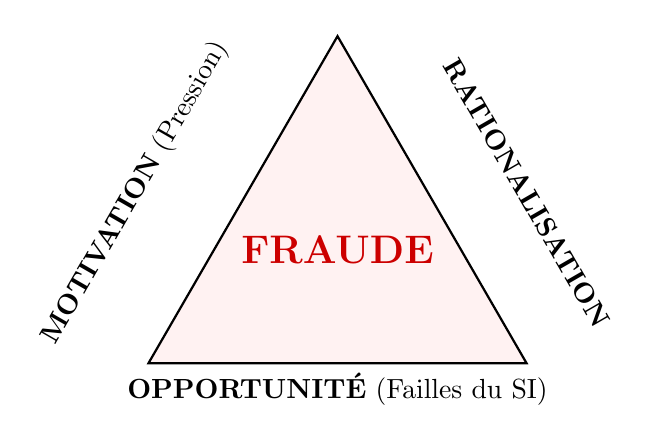
\begin{tikzpicture}[scale=1.2]
    \coordinate (A) at (0,0);
    \coordinate (B) at (4,0);
    \coordinate (C) at (2,3.46);
    
    \draw[thick, fill=red!5] (A) -- (B) -- (C) -- cycle;
    
    \node[below] at (2,0) {\textbf{OPPORTUNITÉ} (Failles du SI)};
    \node[left] at (1,1.8) {\rotatebox{60}{\textbf{MOTIVATION} (Pression)}};
    \node[right] at (3,1.8) {\rotatebox{-60}{\textbf{RATIONALISATION}}};
    
    \node at (2,1.2) {\textcolor{red!80!black}{\Large \textbf{FRAUDE}}};
\end{tikzpicture}
\end{center}


% Chapitre 8 — Évaluation finale
% ==============================================================================
% Fichier : 07_evaluation_finale.tex
% Description : Evaluation Finale du Cours d'Audit des SI
% ==============================================================================

\chapter{Évaluation Finale du Cours}\label{chap:08_evaluation_finale}

Cette évaluation valide l'acquisition des concepts fondamentaux de l'audit, la maîtrise de la démarche méthodologique et la connaissance des référentiels.

% ------------------------------------------------------------------------------
\section{Partie A : QCM (Choix Multiples)}
% ------------------------------------------------------------------------------

\textbf{Consigne :} Cochez la ou les bonnes réponses.

\subsection*{Chapitre 2 : Fondamentaux}
\begin{enumerate}
    \item L'audit a pour sujet principal :
    \begin{itemize} \item[A.] Une opération unitaire. \item[B.] Un processus global. \item[C.] Un employé précis. \item[D.] Une transaction financière. \end{itemize}
    \item Le "Risque Résiduel" est :
    \begin{itemize} \item[A.] Le risque avant toute mesure de sécurité. \item[B.] Le risque qui reste après l'application des contrôles. \item[C.] Un risque qui ne peut pas se produire. \item[D.] Le risque de l'auditeur de se tromper. \end{itemize}
    \item La règle des "Quatre Yeux" signifie :
    \begin{itemize} \item[A.] Avoir quatre yeux (mutation génétique). \item[B.] Qu'une opération sensible doit être validée par deux personnes distinctes. \item[C.] Relire un document quatre fois. \item[D.] Avoir deux superviseurs. \end{itemize}
    \item Un contrôle "Préventif" a pour but de :
    \begin{itemize} \item[A.] Détecter l'erreur après coup. \item[B.] Empêcher l'erreur ou la fraude de se produire. \item[C.] Coriger l'erreur. \item[D.] Sanctionner le coupable. \end{itemize}
    \item L'assurance fournie par un audit est dite "Raisonnable" car :
    \begin{itemize} \item[A.] L'auditeur est gentil. \item[B.] Elle n'est pas absolue (limites de l'échantillonnage et du temps). \item[C.] Elle est garantie à 100\%. \item[D.] Elle dépend du prix payé. \end{itemize}
\end{enumerate}

\subsection*{Chapitre 3 : Démarche et Normes}
\begin{enumerate}
    \setcounter{enumi}{5}
    \item La norme qui encadre la méthodologie de l'audit est :
    \begin{itemize} \item[A.] ISO 27001. \item[B.] ISO 19011. \item[C.] COBIT. \item[D.] COSO. \end{itemize}
    \item Le principe de "Confidentialité" pour l'auditeur signifie :
    \begin{itemize} \item[A.] Ne rien dire à personne. \item[B.] Protéger les informations sensibles découvertes. \item[C.] Cacher les résultats à la direction. \item[D.] Signer un accord de non-divulgation. \end{itemize}
    \item Le "Rapport d'Orientation" est validé par :
    \begin{itemize} \item[A.] L'auditeur. \item[B.] L'audité. \item[C.] Le Commanditaire (PDG/COMEX). \item[D.] Le fournisseur informatique. \end{itemize}
    \item La phase de "Contradictoire" permet à l'audité de :
    \begin{itemize} \item[A.] Contester les observations et apporter des preuves nouvelles. \item[B.] Refuser le rapport. \item[C.] Corriger lui-même ses erreurs. \item[D.] Changer l'auditeur. \end{itemize}
    \item Une observation d'audit contient obligatoirement :
    \begin{itemize} \item[A.] Le nom du coupable. \item[B.] Le risque, la cause et le constat. \item[C.] Une amende. \item[D.] Une opinion personnelle. \end{itemize}
\end{enumerate}

\subsection*{Chapitre 4 : Référentiels}
\begin{enumerate}
    \setcounter{enumi}{10}
    \item COSO est un modèle de :
    \begin{itemize} \item[A.] Sécurité réseau. \item[B.] Contrôle Interne. \item[C.] Développement logiciel. \item[D.] Gestion de projet. \end{itemize}
    \item COBIT est un référentiel pour :
    \begin{itemize} \item[A.] La gouvernance et le management des SI. \item[B.] La comptabilité. \item[C.] La sécurité physique. \item[D.] Les ressources humaines. \end{itemize}
    \item La norme certifiable pour la sécurité de l'information est :
    \begin{itemize} \item[A.] ISO 27002. \item[B.] ISO 27001. \item[C.] ISO 27005. \item[D.] ISO 19011. \end{itemize}
    \item Le domaine COBIT "Acquérir et Implémenter" concerne :
    \begin{itemize} \item[A.] L'exploitation quotidienne. \item[B.] Les projets et changements. \item[C.] La stratégie. \item[D.] Le budget. \end{itemize}
    \item Les 5 composantes de COSO incluent :
    \begin{itemize} \item[A.] L'environnement de contrôle. \item[B.] La gestion des stocks. \item[C.] Le marketing. \item[D.] La paie. \end{itemize}
\end{enumerate}

\subsection*{Chapitre 5 : Types d'Audits}
\begin{enumerate}
    \setcounter{enumi}{15}
    \item L'audit d'une application en service vérifie :
    \begin{itemize} \item[A.] La fiabilité et la sécurité des données. \item[B.] Le projet de développement. \item[C.] Les contrats des fournisseurs. \item[D.] L'organigramme de l'entreprise. \end{itemize}
    \item Les "Contrôles Généraux" (General Controls) portent sur :
    \begin{itemize} \item[A.] Une fonction précise du logiciel. \item[B.] L'environnement global (OS, Réseau, Sauvegarde). \item[C.] Une facture spécifique. \item[D.] Un utilisateur unique. \end{itemize}
    \item L'audit de sécurité vérifie le principe DIC/T. La lettre I signifie :
    \begin{itemize} \item[A.] Informatique. \item[B.] Intégrité. \item[C.] Intelligence. \item[D.] Investissement. \end{itemize}
    \item L'audit de projet intervient généralement :
    \begin{itemize} \item[A.] Uniquement après la panne. \item[B.] Pendant le projet (jalons) ou à la fin. \item[C.] Avant le cahier des charges. \item[D.] Jamais. \end{itemize}
    \item Un "Pentest" (Test d'intrusion) est :
    \begin{itemize} \item[A.] Un audit de configuration. \item[B.] Une simulation d'attaque réelle. \item[C.] Une réunion de travail. \item[D.] Un test de performance. \end{itemize}
\end{enumerate}

\subsection*{Chapitre 6 : Sujets Connexes}
\begin{enumerate}
    \setcounter{enumi}{20}
    \item Le risque principal de l'utilisation de l'IA pour l'auditeur est :
    \begin{itemize} \item[A.] L'automatisation. \item[B.] Le biais algorithmique et la "boîte noire". \item[C.] Le coût élevé. \item[D.] La rapidité. \end{itemize}
    \item La fraude "interne" est commise par :
    \begin{itemize} \item[A.] Un concurrent. \item[B.] Un employé de l'entreprise. \item[C.] Un client. \item[D.] Un hacker étranger. \end{itemize}
    \item La "Séparation des Tâches" est un contrôle :
    \begin{itemize} \item[A.] Correctif. \item[B.] Détectif. \item[C.] Préventif. \item[D.] Technique. \end{itemize}
    \item Pour détecter une fraude, l'auditeur utilise souvent :
    \begin{itemize} \item[A.] L'intuition. \item[B.] L'analyse de données (Data Mining). \item[C.] Les rumeurs. \item[D.] La voyance. \end{itemize}
    \item La ligne éthique (Whistleblowing) sert à :
    \begin{itemize} \item[A.] Signaler anonymement des comportements suspects. \item[B.] Commander du matériel. \item[C.] Gérer les mots de passe. \item[D.] Contacter le support. \end{itemize}
\end{enumerate}

% ------------------------------------------------------------------------------
\section{Partie B : Vrai ou Faux}
% ------------------------------------------------------------------------------

\textbf{Consigne :} Justifiez si faux (optionnel).

\begin{enumerate}
    \item L'auditeur interne est obligatoirement un employé de l'entreprise. \textbf{(Vrai)}
    \item Un contrôle détectif empêche la fraude de se produire. \textbf{(Faux - Il la détecte après coup)}
    \item L'indépendance est un principe éthique obligatoire pour l'auditeur. \textbf{(Vrai)}
    \item Le rapport d'audit est la seule production de l'auditeur. \textbf{(Faux - Il y a les papiers de travail, le rapport d'orientation...)}
    \item COSO est un référentiel réservé à l'informatique. \textbf{(Faux - C'est un modèle de contrôle interne généraliste)}
    \item ISO 27002 contient les exigences de certification. \textbf{(Faux - C'est ISO 27001, l'ISO 27002 est un guide de bonnes pratiques)}
    \item L'audit d'application vérifie uniquement le code source. \textbf{(Faux - Il vérifie les données, les processus et l'environnement)}
    \item Le "Suivi d'audit" (Follow-up) sert à vérifier l'application des recommandations. \textbf{(Vrai)}
    \item L'IA peut être utilisée comme outil d'aide à l'audit. \textbf{(Vrai)}
    \item Le principe de "Présentation équitable" permet à l'auditeur de mentir pour protéger l'entreprise. \textbf{(Faux - Il doit être honnête et factuel)}
\end{enumerate}

% ------------------------------------------------------------------------------
\section{Partie C : Questions Ouvertes}
% ------------------------------------------------------------------------------

\textbf{Consigne :} Répondez en 10-15 lignes.

\begin{enumerate}
    \item Expliquez la différence fondamentale entre l'Approche fondée sur les risques et l'Approche fondée sur les contrôles en audit.
    \item Quels sont les 5 composantes du référentiel COSO et quel est leur lien ?
    \item Décrivez les 3 phases principales de la relation avec l'audité lors d'une mission (Ouverture, Terrain, Clôture).
    \item Pourquoi la "Charte d'Audit" est-elle un document indispensable pour l'auditeur interne ?
    \item Comparez les objectifs d'un "Audit de Sécurité" et d'un "Audit de Performance".
    \item Quels sont les risques spécifiques liés à l'intégration de l'Intelligence Artificielle dans les SI que l'auditeur doit vérifier ?
    \item Expliquez le principe de séparation des tâches (Règle des deux mains) avec un exemple concret.
\end{enumerate}

% ------------------------------------------------------------------------------
\section{Partie D : Cas Pratique (Étude de Cas)}
% ------------------------------------------------------------------------------

\subsection{Scénario : Audit de l'Application "Comptabilité" de Lizbiz's}

\begin{displayquote}
Vous êtes l'auditeur senior mandaté pour auditer le module comptabilité de l'APPLICATION de Lizbiz's.
Lors de vos tests, vous constatez les faits suivants :
\begin{enumerate}
    \item L'administrateur système "Root" a accès directement à la base de données financières sans passer par l'application.
    \item Les sauvegardes journalières sont stockées sur un disque dur USB posé sur le bureau du comptable.
    \item Le comptable principal part en vacances et donne son mot de passe à son stagiaire pour qu'il continue le travail.
\end{enumerate}
\end{displayquote}

\textbf{Travaux demandés :}

\begin{enumerate}
    \item Pour chaque fait constaté, identifiez :
    \begin{itemize}
        \item Le risque encouru par Lizbiz's.
        \item Le type de contrôle défaillant (Préventif, Détectif, organisationnel, technique).
    \end{itemize}
    \item Rédigez une recommandation appropriée pour le constat n°3 (Partage de mot de passe).
    \item En vous référant à ISO 27001, citez un domaine de l'Annexe A qui aurait permis d'éviter le constat n°2 (Sauvegardes).
\end{enumerate}


% -------------------------------------------------------------------
% TRAVAUX PRATIQUES (Laboratoires)
% -------------------------------------------------------------------
\part{Travaux Pratiques Immersifs}

% ==============================================================================
% Fichier : lab1_application.tex
% Description : Laboratoire 1 - Audit d'une Application Comptable (APPLICATION)
% ==============================================================================

\chapter{Laboratoire 1 : Audit d'une Application en Service}\label{chap:lab1_application}

Ce laboratoire met en pratique la méthodologie d'audit sur le cas de l'application comptable de l'entreprise LiZbiZ, nommée \textbf{APPLICATION}. L'objectif est de simuler une mission réelle : revue de contrôle interne, tests de données et rédaction de rapport.

\section{Objectifs du TP}
\begin{itemize}
    \item Créer et peupler l'environnement technique (Base de données).
    \item Concevoir les outils d'audit (Grilles de contrôle).
    \item Réaliser des tests de contrôles et des tests substantifs via SQL.
    \item Rédiger le rapport d'audit final.
\end{itemize}

% ------------------------------------------------------------------------------
\section{Étape 1 : Préparation de l'Environnement (Base de Données)}
% ------------------------------------------------------------------------------

Avant d'auditer, il faut disposer du système. Nous allons créer le schéma de la base de données de l'APPLICATION.

\subsection{Création du Schéma Relationnel}

Exécutez le script SQL suivant sur votre SGBD (PostgreSQL ou MySQL).

\begin{lstlisting}[language=SQL, caption=Script de création de la base APPLICATION]
-- Creation des tables

CREATE TABLE UTILISATEUR (
    IdUser INT PRIMARY KEY,
    Nom VARCHAR(50),
    Prenom VARCHAR(50),
    Service VARCHAR(50),
    Profil VARCHAR(20), -- 'Admin', 'Comptable', 'Validation'
    Actif BOOLEAN
);

CREATE TABLE JOURNAL (
    CodeJournal VARCHAR(5) PRIMARY KEY,
    Libelle VARCHAR(50)
);

CREATE TABLE COMPTE (
    NumCompte VARCHAR(10) PRIMARY KEY,
    Libelle VARCHAR(100),
    Classe VARCHAR(2)
);

CREATE TABLE TIERS (
    IdTiers INT PRIMARY KEY,
    Nom VARCHAR(100),
    Type VARCHAR(20), -- 'Client', 'Fournisseur'
    Email VARCHAR(100)
);

CREATE TABLE ECRITURE (
    IdEcriture INT PRIMARY KEY,
    DateEcriture DATE,
    CodeJournal VARCHAR(5),
    NumCompte VARCHAR(10),
    IdTiers INT,
    Libelle VARCHAR(200),
    Debit DECIMAL(15,2),
    Credit DECIMAL(15,2),
    IdUserCreate INT,
    IdUserValid INT, -- Utilisateur qui valide
    Statut VARCHAR(10), -- 'Brouillon', 'Valide'
    FOREIGN KEY (CodeJournal) REFERENCES JOURNAL(CodeJournal),
    FOREIGN KEY (NumCompte) REFERENCES COMPTE(NumCompte),
    FOREIGN KEY (IdTiers) REFERENCES TIERS(IdTiers)
);
\end{lstlisting}

\subsection{Chargement des Données de Test}

Insérez un jeu de données fictives pour simuler l'activité de LiZbiZ. (Voir annexe du PDF source pour un jeu complet ou générez-en un simplifié).

\begin{lstlisting}[language=SQL, caption=Exemple d'insertion]
-- Insertion des utilisateurs
INSERT INTO UTILISATEUR VALUES (1, 'DUPONT', 'Marie', 'Comptabilite', 'Comptable', TRUE);
INSERT INTO UTILISATEUR VALUES (2, 'MARTIN', 'Paul', 'Direction', 'Validation', TRUE);
INSERT INTO UTILISATEUR VALUES (3, 'HACK', 'Bad', 'IT', 'Admin', TRUE);

-- Insertion d'une ecriture suspecte (Fraude potentielle)
INSERT INTO ECRITURE VALUES (1001, '2023-12-15', 'ACH', '607', 50, 'Achat Fictif', 5000, 0, 1, 1, 'Valide');
\end{lstlisting}

% ------------------------------------------------------------------------------
\section{Étape 2 : Évaluation du Contrôle Interne (COSO)}
% ------------------------------------------------------------------------------

L'objectif est de concevoir la "Checklist" d'audit.

\subsection{Domaine : Environnement de Contrôle}

Concevez un questionnaire d'évaluation pour vérifier la culture sécurité du service comptabilité de LiZbiZ.
\textbf{Questions à formuler :}
\begin{itemize}
    \item Existe-t-il une charte informatique signée par les comptables ?
    \item Les utilisateurs connaissent-ils leur profil d'accès ?
    \item Qui a le profil "Admin" sur l'application ?
\end{itemize}

\subsection{Domaine : Activités de Contrôle (Séparation des Tâches)}

C'est le point critique. Vérifiez la matrice RACI.
\textbf{Tâche :} Vérifier si un même utilisateur peut créer ET valider une écriture (Risque de fraude majeur).

\begin{boxlizbiz}
\textbf{Requête SQL de vérification (Audit Technique) :}
Ecrire une requête pour détecter les utilisateurs qui ont créé une écriture et l'ont eux-mêmes validée.
\begin{lstlisting}[language=SQL]
SELECT IdEcriture, Libelle, IdUserCreate 
FROM ECRITURE 
WHERE IdUserCreate = IdUserValid;
\end{lstlisting}
\textbf{Analyse :} Si le résultat n'est pas vide, c'est une Non-Conformité Majeure (Règle des 4 yeux non respectée).
\end{boxlizbiz}

% ------------------------------------------------------------------------------
\section{Étape 3 : Audit des Données (Tests Substantifs)}
% ------------------------------------------------------------------------------

Nous utilisons le langage SQL comme outil d'audit (CAATs - Computer Assisted Audit Techniques).

\subsection{Test d'Intégrité : Recherche de Doublons}

\textbf{Risque :} Factures payées deux fois.
\textbf{Objectif :} Détecter les écritures strictement identiques (même montant, même date, même tiers, même libellé).

\begin{lstlisting}[language=SQL]
SELECT DateEcriture, IdTiers, Libelle, Sum(Debit) as TotalDebit, Count(*) as NbOcurrences
FROM ECRITURE
GROUP BY DateEcriture, IdTiers, Libelle
HAVING Count(*) > 1;
\end{lstlisting}

\subsection{Test de Cohérence : Equilibre Journal}

\textbf{Risque :} Déséquilibre comptable.
\textbf{Objectif :} Vérifier que Total Débit = Total Crédit pour chaque journal.

\begin{lstlisting}[language=SQL]
SELECT CodeJournal, SUM(Debit) as TotalD, SUM(Credit) as TotalC
FROM ECRITURE
GROUP BY CodeJournal
HAVING SUM(Debit) != SUM(Credit);
\end{lstlisting}

\subsection{Test de Convention : Seuil de Validation}

\textbf{Règle de gestion LiZbiZ :} Toute écriture supérieure à 5000 € doit être validée par le Directeur (Profil 'Validation').
\textbf{Objectif :} Détecter les écritures > 5000 € validées par un simple comptable.

\begin{lstlisting}[language=SQL]
SELECT E.IdEcriture, E.Libelle, E.Debit, U.Nom as Validateur, U.Profil
FROM ECRITURE E
JOIN UTILISATEUR U ON E.IdUserValid = U.IdUser
WHERE E.Debit > 5000 AND U.Profil != 'Validation';
\end{lstlisting}

% ------------------------------------------------------------------------------
\section{Étape 4 : Rapport d'Audit}
% ------------------------------------------------------------------------------

\subsection{Rédaction des Observations}

Sur la base des requêtes exécutées, rédigez une fiche d'observation pour le rapport final (Format : Constat / Risque / Recommandation).

\textbf{Exemple de fiche à compléter :}

\begin{table}[h!]
\centering
\small
\begin{tabular}{|p{3cm}|p{9cm}|}
    \hline
    \textbf{Titre} & Non respect de la séparation des tâches (Création/Validation). \\
    \hline
    \textbf{Constat} & La requête SQL a identifié X écritures validées par leur créateur. \\
    \hline
    \textbf{Risque} & Fraude interne sans contrôle (Détournement possible). \\
    \hline
    \textbf{Recommandation} & Configurer l'APPLICATION pour interdire l'auto-validation (Bloquer l'enregistrement si IdUserCreate = IdUserValid). \\
    \hline
\end{tabular}
\caption{Modèle de fiche d'observation}
\end{table}

% ------------------------------------------------------------------------------
\section{Livrables à rendre}
% ------------------------------------------------------------------------------

\begin{enumerate}
    \item Le script SQL de création de la base (Fichier .sql).
    \item Le fichier Excel ou Word contenant les grilles de contrôle interne.
    \item Les scripts SQL utilisés pour les tests (Audit des données).
    \item Le rapport d'audit final (PDF) contenant les observations et le plan d'action.
\end{enumerate}

% ==============================================================================
% Fichier : lab2_infrastructure.tex
% Description : Laboratoire 2 - Audit de Sécurité d'une Infrastructure
% ==============================================================================

\chapter{Laboratoire 2 : Audit de Sécurité d'une Infrastructure}\label{chap:lab2_infrastructure}

Ce laboratoire complète l'audit fonctionnel par une approche technique. L'objectif est d'évaluer la sécurité du réseau et des systèmes de l'entreprise LiZbiZ pour détecter les vulnérabilités exploitables par un attaquant.

\section{Objectifs du TP}
\begin{itemize}
    \item Analyser une architecture réseau pour valider la segmentation.
    \item Réaliser un audit de configuration (pare-feu, services).
    \item Utiliser des outils d'audit standards (Nmap, scanners de vulnérabilités).
    \item Produire un rapport technique d'audit infrastructure.
\end{itemize}

% ------------------------------------------------------------------------------
\section{Étape 1 : Analyse de l'Architecture (Revue Documentaire)}
% ------------------------------------------------------------------------------

\subsection{Présentation de l'Infrastructure LiZbiZ}

L'infrastructure cible est modélisée sous GNS3 ou EVE-NG. Elle est composée de trois zones principales :

\begin{itemize}
    \item \textbf{VLAN 10 (DMZ) :} Serveur Web Public (Accessibilité Internet).
    \item \textbf{VLAN 20 (Applicatif) :} Serveur ERP, Base de Données.
    \item \textbf{VLAN 30 (Utilisateurs) :} Postes de travail, Active Directory.
\end{itemize}

\subsection{Travail Demandé : Analyse de la Cartographie}

À partir du schéma fourni (ou de la simulation), répondez aux questions suivantes :
\begin{enumerate}
    \item Le serveur Web en DMZ a-t-il un accès direct au VLAN Utilisateurs ? (Risque : pivot depuis le web vers les postes).
    \item La Base de Données est-elle accessible depuis Internet ? (Risque : exposition des données).
    \item Les protocoles d'administration (SSH, Telnet, RDP) sont-ils autorisés entre toutes les zones ?
\end{enumerate}

\begin{boxalert}
\textbf{Attention :} Une architecture correcte doit interdire tout flux direct Internet $\rightarrow$ BDD. Le flux doit passer par le Serveur Web (Proxy).
\end{boxalert}

% ------------------------------------------------------------------------------
\section{Étape 2 : Découverte et Cartographie Réelle (Nmap)}
% ------------------------------------------------------------------------------

L'auditeur ne se fie pas uniquement aux schémas théoriques. Il doit scanner le réseau pour voir la réalité technique ("Shadow IT" potentiel).

\subsection{Scan de Découverte}

Utilisez l'outil \textbf{Nmap} depuis une machine attaquante (ex: Kali Linux) placée en position externe (simulant Internet) ou interne (simulant un poste utilisateur compromis).

\textbf{Commande de base :}
\begin{lstlisting}[language=bash, caption=Scan réseau Nmap]
# Scan rapide pour voir les hotes actifs
nmap -sn 192.168.1.0/24

# Scan des ports ouverts sur le serveur Web
nmap -sV -p- 192.168.1.10 (IP Serveur Web)
\end{lstlisting}

\subsection{Questions d'Audit}
\begin{itemize}
    \item \textbf{Question 1 :} Quels ports sont ouverts sur le serveur Web ? (Attendu : 80/443. Risque : 22, 21, 3389 ouverts).
    \item \textbf{Question 2 :} Le pare-feu bloque-t-il les pings (ICMP) ? (Mesure de sécurité basique).
    \item \textbf{Question 3 :} Identifiez-vous des services vulnérables (ex: FTP non chiffré, vieux Apache) ?
\end{itemize}

% ------------------------------------------------------------------------------
\section{Étape 3 : Audit de Configuration et Vulnérabilités}
% ------------------------------------------------------------------------------

\subsection{Test de Segmentation (Bypass Pare-feu)}

\textbf{Objectif :} Vérifier que le VLAN Utilisateur ne peut pas accéder directement au port d'administration de la Base de Données (ex: port 3306 ou 5432).

\textbf{Action :} Depuis une machine du VLAN 30, tentez de vous connecter au port SQL du VLAN 20.
\begin{lstlisting}[language=bash]
telnet <IP_SERVEUR_DB> 3306
# Si la connexion s'ouvre -> ECHEC DU CONTROLE (Segmentation inexistante).
\end{lstlisting}

\subsection{Scan de Vulnérabilités (OpenVAS / Nessus)}

Lancez un scan de vulnérabilités sur le serveur Web (DMZ).
\textbf{Analyse des résultats :}
\begin{itemize}
    \item Classez les vulnérabilités par sévérité (Critical, High, Medium).
    \item Identifiez les failles connues (CVE) non patchées.
\end{itemize}

\begin{boxlizbiz}
\textbf{Cas Lizbiz's :}
Le scan révèle que le serveur Web exécute une version d'Apache datant de 2018 (CVE critique présente).
\textbf{Constat :} Le processus de mise à jour (Patch Management) est défaillant.
\textbf{Risque :} Prise de contrôle totale du serveur par un attaquant externe.
\end{boxlizbiz}

% ------------------------------------------------------------------------------
\section{Étape 4 : Analyse des Configurations (Hardening)}
% ------------------------------------------------------------------------------

\subsection{Audit des Comptes par Défaut}

Connectez-vous aux équipements (Routeur/Firewall) ou aux services (Base de données).
Vérifiez :
\begin{itemize}
    \item Est-ce que le compte "admin" / "admin" fonctionne encore ?
    \item Est-ce que le compte "root" de la base de données a un mot de passe vide ?
\end{itemize}

\subsection{Audit des Protocoles}

\begin{table}[h!]
\centering
\begin{tabular}{p{4cm}p{4cm}p{4cm}}
    \toprule
    \textbf{Service} & \textbf{Configuration Sécurisée} & \textbf{Configuration Observée} \\
    \midrule
    Administration Réseau & SSH (v2) & Telnet (Clair) ? \\
    Transfert Fichier & SFTP / SCP & FTP (Clair) ? \\
    Accès Web & HTTPS & HTTP ? \\
    \bottomrule
\end{tabular}
\caption{Grille de vérification des protocoles}
\end{table}

% ------------------------------------------------------------------------------
\section{Étape 5 : Rapport d'Audit Technique}
% ------------------------------------------------------------------------------

\subsection{Synthèse des Risques}

Résumez les risques majeurs identifiés (Impact Technique $\rightarrow$ Impact Métier).

\subsection{Plan de Remédiation}

Proposez un plan d'action technique pour LiZbiZ (Exemples : "Fermer le port 22 sur la DMZ", "Migrer de HTTP à HTTPS", "Appliquer les mises à jour de sécurité").

% ------------------------------------------------------------------------------
\section{Livrables à Rendre}
% ------------------------------------------------------------------------------

\begin{enumerate}
    \item Fichier Nmap (format XML ou texte) montrant les résultats du scan.
    \item Tableau d'analyse de la segmentation (Matrice de flux autorisés vs observés).
    \item Rapport d'audit technique avec classification des vulnérabilités (CVSS).
\end{enumerate}



% --- Conclusion Générale ---
% ==============================================================================
% Fichier     : chapitres/00_Conclusion.tex
% Titre       : Conclusion Générale du Cours d'Audit des Systèmes d'Information
% Auteur      : MINKA MI NGUIDJOÏ Thierry Emmanuel
% ==============================================================================

\chapter*{Conclusion Générale}\label{chap:conclusion}
\addcontentsline{toc}{chapter}{Conclusion Générale}
\markboth{Conclusion Générale}{Conclusion Générale}

\begin{flushright}
    \itshape
    <<~L'audit est terminé lorsque le dernier doute raisonnable\\
    a été levé, documenté et communiqué.~>>\\[0.5ex]
    \small--- Principe fondateur de l'IIA
\end{flushright}

\vspace{1.5ex}

% ==============================================================================
\section*{Ce que Vous Avez Appris}
% ==============================================================================

Au terme de ce parcours, vous avez traversé l'intégralité du spectre de l'audit des systèmes d'information — des fondements conceptuels aux tests techniques, du vocabulaire professionnel à la rédaction du rapport final. Ce cheminement n'était pas linéaire dans sa nature : il était \textit{spiralaire}, chaque niveau de compréhension enrichissant rétrospectivement les acquis antérieurs.

Vous avez appris à distinguer ce que l'on \textbf{contrôle} de ce que l'on \textbf{audite}, à mesurer un \termecle{risque résiduel} plutôt qu'à fantasmer un risque zéro, à lire un SI non comme une boîte noire mais comme un \textit{système de contrôles imbriqués} dont la solidité se mesure au maillon le plus faible.

Vous avez découvert que l'auditeur moderne n'est pas seulement un expert technique : il est un \textbf{traducteur} entre le monde de la machine et celui de la décision stratégique, capable de transformer des lignes de logs en recommandations compréhensibles par un comité de direction.

% ==============================================================================
\section*{Synthèse des Compétences Acquises}
% ==============================================================================

\begin{boxresume}
Les compétences fondamentales consolidées au cours de cette formation :

\begin{enumerate}
    \item \textbf{Maîtrise du cadre conceptuel :} Distinction audit / contrôle, assurance raisonnable, cycle du risque, contrôle interne (COSO).
    \item \textbf{Connaissance des référentiels :} COBIT, ISO 27001/27002, ISO 19011 comme grilles d'évaluation universelles.
    \item \textbf{Conduite d'une mission :} Planification, exécution (tests documentaires, entretiens, tests techniques), rédaction du rapport contradictoire.
    \item \textbf{Audit technique :} Requêtes SQL d'analyse de données, scan réseau (Nmap), audit de configuration, détection de vulnérabilités.
    \item \textbf{Enjeux émergents :} Gouvernance de l'IA, détection de la fraude numérique, protection des données personnelles (RGPD).
    \item \textbf{Communication professionnelle :} Rédaction de constats, d'observations et de plans d'action à destination de la direction générale.
\end{enumerate}
\end{boxresume}

% ==============================================================================
\section*{Le Cas LiZbiZ : Bilan de la Mission}
% ==============================================================================

L'entreprise LiZbiZ a constitué tout au long de ce cours le terrain d'application de votre apprentissage. À travers elle, vous avez rencontré des situations que tout auditeur croisera inévitablement dans sa carrière : une application comptable dont la piste d'audit était défaillante, une infrastructure réseau mal segmentée exposant la base de données, un projet d'IA dont les données d'entraînement étaient contaminées, des rumeurs de fraude aux fournisseurs fictifs transformées en constats documentés.

\begin{boxlizbiz}
\textbf{Bilan de la mission LiZbiZ :}
\begin{itemize}
    \item \textbf{Observations critiques identifiées :} Absence de piste d'audit sur le module comptable ; segmentation réseau inefficace ; serveur Apache non patché (CVE critique) ; présence de comptes fournisseurs suspects.
    \item \textbf{Niveau de risque résiduel global :} \textcolor{red}{\textbf{Élevé}} — justifiant un suivi de recommandations à 30, 90 et 180 jours.
    \item \textbf{Recommandation principale :} Mise en place d'un programme de contrôle interne continu (COSO Pilotage) et certification ISO 27001 à 18 mois.
\end{itemize}
\end{boxlizbiz}

% ==============================================================================
\section*{Perspectives Professionnelles}
% ==============================================================================

L'audit des SI est l'une des disciplines dont la demande ne cesse de croître à mesure que la transformation numérique s'accélère. Les certifications \sigle{CISA} (\textit{Certified Information Systems Auditor}), \sigle{CISM} (\textit{Certified Information Security Manager}) et \sigle{CRISC} (\textit{Certified in Risk and Information Systems Control}), délivrées par l'\sigle{ISACA}, constituent les références mondiales du secteur. Elles ouvrent les portes des cabinets d'audit des quatre plus grands (Deloitte, PwC, EY, KPMG), des institutions publiques de contrôle supérieur, et des directions d'audit interne des grandes organisations.

\begin{boxinfo}
\textbf{Pour aller plus loin :}
\begin{itemize}
    \item \textit{ISACA — CISA Review Manual}, édition courante.
    \item \textit{IIA — International Standards for the Professional Practice of Internal Auditing}.
    \item \textit{ISO/IEC 27001:2022 — Systèmes de management de la sécurité de l'information}.
    \item \textit{NIST Cybersecurity Framework} (v2.0, 2024).
    \item Revue \textit{ISACA Journal} — articles pratiques et cas d'études sectoriels.
\end{itemize}
\end{boxinfo}

% ==============================================================================
\section*{Mot Final}
% ==============================================================================

L'audit n'est pas une fin en soi. C'est un instrument au service d'une ambition plus haute : permettre aux organisations d'apprendre d'elles-mêmes, de se corriger avec lucidité et de construire une confiance durable avec leurs parties prenantes. Dans un monde où l'information est la ressource la plus précieuse et la plus vulnérable à la fois, l'auditeur SI est, plus que jamais, un gardien de la confiance numérique.

Que vous exerciez demain en cabinet, en institution publique ou au sein d'une direction de l'audit interne, portez cette conviction : \textit{un constat bien documenté vaut mieux qu'une intuition brillante}. La rigueur est votre crédibilité. L'indépendance, votre autorité.

\vspace{2ex}
\begin{center}
    {\color{CouleurAccent}\rule{0.6\linewidth}{1pt}}\\[0.8ex]
    {\small\itshape\color{CouleurPrimaire}
        Rédigé et enseigné avec la conviction que la maîtrise du numérique\\
        est une responsabilité collective autant qu'individuelle.}\\[0.5ex]
    {\small\bfseries\color{CouleurPrimaire}\auteurcours}\\
    {\footnotesize\color{CouleurBordInfo}\itshape\institutionprimaire{} --- \anneescolaire}
\end{center}


% ==============================================================================
% MATIÈRE POSTLIMINAIRE
% ==============================================================================
\backmatter

% --- Bibliographie ---
\clearpage
\printbibliography[
    heading=bibintoc,
    title={Bibliographie et Références}
]

% --- À Propos de l'Auteur ---
\clearpage
%% ==============================================================================
% Fichier     : chapitres/Apropos_Auteur.tex
% Titre       : À Propos de l'Auteur
% Auteur      : MINKA MI NGUIDJOÏ Thierry Emmanuel
% ==============================================================================

\chapter*{À Propos de l'Auteur}
\addcontentsline{toc}{chapter}{À Propos de l'Auteur}
\markboth{À Propos de l'Auteur}{À Propos de l'Auteur}

\vspace{1ex}

% Bandeau décoratif supérieur
\begin{tcolorbox}[
    enhanced,
    colback=CouleurPrimaire,
    colframe=CouleurPrimaire,
    arc=0pt,
    boxrule=0pt,
    left=0pt, right=0pt, top=4pt, bottom=4pt
]
\centering
{\color{CouleurAccent}\rule{0.3\linewidth}{0.8pt}}\quad
{\color{white}\large\bfseries MINKA MI NGUIDJOÏ Thierry Emmanuel}\quad
{\color{CouleurAccent}\rule{0.3\linewidth}{0.8pt}}\\[2pt]
{\color{white!80!gray}\small\itshape
    Chercheur~$\cdot$~Expert en Sécurité de l'Information~$\cdot$~Enseignant}
\end{tcolorbox}

\vspace{1.5ex}

% ==============================================================================
% BLOC BIOGRAPHIE PRINCIPALE
% ==============================================================================

\begin{tcolorbox}[
    enhanced,
    breakable,
    colback=white,
    colframe=CouleurSecondaire,
    arc=4pt,
    boxrule=1pt,
    left=10pt, right=10pt, top=10pt, bottom=10pt
]

\textbf{MINKA MI NGUIDJOÏ Thierry Emmanuel} est chercheur au \termecle{Laboratoire d'Informatique et de Mathématiques pour les Sciences de l'Ingénieur} (\sigle{LIMSI}) de l'Université de Yaoundé~I, au Cameroun. Ses travaux de doctorat, conduits sous la double direction du Professeur \textbf{Flavien Serge Mani Onana} et du Professeur \textbf{Thomas Djotio Ndié}, portent sur les fondements formels de la \termecle{cryptographie institutionnelle} — une discipline qu'il a lui-même fondée et dont il est l'initiateur reconnu au sein de la communauté scientifique internationale.

\medskip

Sa thèse, intitulée \textit{«~Aux fondements de la cryptographie institutionnelle~: formalisation, bornes d'impossibilité, conditions d'optimalité et vérification formelle~»}, articule des contributions théoriques majeures autour du \textbf{Cadre CLO} (\textit{Confidentiality-Legibility-Opacity}), du \textbf{Trilemme CRO} (\textit{Confidentiality-Recoverability-Opacity}), de la \textbf{Famille SOTP} (\textit{State-based One-Time Protocols}) et des extensions post-quantiques qui en découlent. Ces travaux, formalisés en partie avec l'assistant de preuve \textbf{Lean 4}, ont donné lieu à neuf prépublications sur l'\sigle{IACR ePrint Archive} et à plusieurs articles publiés dans \textit{IEEE Access}.

\end{tcolorbox}

\vspace{1ex}

% ==============================================================================
% DEUX COLONNES : PARCOURS ET CERTIFICATIONS
% ==============================================================================

\begin{minipage}[t]{0.52\textwidth}
\begin{tcolorbox}[
    enhanced,
    colback=CouleurDef,
    colframe=CouleurBordDef,
    fonttitle=\bfseries\color{white},
    title={\textbf{[\S]}\quad Parcours Académique et Institutionnel},
    attach boxed title to top left={yshift=-2mm, xshift=4mm},
    boxed title style={colback=CouleurBordDef, rounded corners},
    arc=3pt, boxrule=0.8pt,
    left=6pt, right=6pt, top=8pt, bottom=6pt
]
\begin{itemize}
    \item \textbf{Doctorant} en Informatique\\
          {\footnotesize Université de Yaoundé~I — \sigle{LIMSI}\\
          \textit{Soutenance prévue : juin 2026}}
    \item \textbf{Chercheur associé} en cryptographie\\
          {\footnotesize Formalisation sous Lean 4, preuves post-quantiques}
    \item \textbf{Enseignant} --- Investigation Numérique\\
          {\footnotesize Cours dispensé en cycle d'ingénierie informatique}
    \item \textbf{Responsable SSI} --- Projet GIP Bénin\\
          {\footnotesize Gouvernance et sécurité des SI publics}
    \item \textbf{Cadre supérieur} --- Contrôle Supérieur de l'État\\
          {\footnotesize Institution supérieure d'audit — République du Cameroun}
\end{itemize}
\end{tcolorbox}
\end{minipage}
\hfill
\begin{minipage}[t]{0.44\textwidth}
\begin{tcolorbox}[
    enhanced,
    colback=CouleurLizbiz,
    colframe=CouleurBordLizbiz,
    fonttitle=\bfseries\color{white},
    title={\ding{166}\quad Certifications Professionnelles},
    attach boxed title to top left={yshift=-2mm, xshift=4mm},
    boxed title style={colback=CouleurBordLizbiz, rounded corners},
    arc=3pt, boxrule=0.8pt,
    left=6pt, right=6pt, top=8pt, bottom=6pt
]
\begin{itemize}
    \item \textbf{\sigle{CISA}}\\
          {\footnotesize \textit{Certified Information Systems Auditor}}
    \item \textbf{\sigle{CISM}}\\
          {\footnotesize \textit{Certified Information Security Manager}}
    \item \textbf{\sigle{CGEIT}}\\
          {\footnotesize \textit{Certified in the Governance of Enterprise IT}}
    \item \textbf{\sigle{CRISC}}\\
          {\footnotesize \textit{Certified in Risk \& Information Systems Control}}
    \item \textbf{\sigle{CDPSE}}\\
          {\footnotesize \textit{Certified Data Privacy Solutions Engineer}}
\end{itemize}
{\footnotesize\color{CouleurBordInfo}\itshape
Toutes certifications délivrées par l'\textbf{ISACA} — l'organisation mondiale de référence en gouvernance, audit et sécurité des SI.}
\end{tcolorbox}
\end{minipage}

\vspace{1.5ex}

% ==============================================================================
% CONTRIBUTIONS SCIENTIFIQUES
% ==============================================================================

\begin{tcolorbox}[
    enhanced,
    colback=white,
    colframe=CouleurAccent,
    fonttitle=\bfseries\color{white},
    title={\ding{167}\quad Contributions Scientifiques Sélectionnées},
    attach boxed title to top left={yshift=-2mm, xshift=4mm},
    boxed title style={colback=CouleurAccent, rounded corners},
    arc=3pt, boxrule=0.8pt,
    left=8pt, right=8pt, top=10pt, bottom=8pt
]

\begin{itemize}
    \item \textbf{P1 — Cadre CLO} : \textit{A Formal Framework for Institutional Cryptography: The CLO Model}\\
          {\footnotesize IEEE Access, pp.~20427--20445, DOI:~\texttt{10.1109/ACCESS.2026.3660105}}

    \item \textbf{P2 — Trilemme CRO} : \textit{The CRO Trilemma: Impossibility Bounds in Institutional Cryptographic Protocols}\\
          {\footnotesize IEEE Access, pp.~33263--33274, DOI:~\texttt{10.1109/ACCESS.2026.3669065}}

    \item \textbf{S1 — Extension PQ-CRO} : Extension post-quantique du Trilemme CRO\\
          {\footnotesize \textit{Soumis à IEEE Access} --- MS-ID:~\texttt{Access-2026-09464}}

    \item \textbf{S2 — Famille SOTP} : \textit{The SOTP Protocol Family: State-based One-Time Protocols}\\
          {\footnotesize \textit{Soumis à IEEE Access} --- MS-ID:~\texttt{Access-2026-09012}}

    \item \textbf{Neuf prépublications} disponibles sur l'\textbf{IACR ePrint Archive}\\
          {\footnotesize Couvrant les primitives CEE, AOW, ZK-NR, Q2CSI, AIIP et les formalisations Lean~4}
\end{itemize}

\end{tcolorbox}

\vspace{1ex}

% ==============================================================================
% GENÈSE DE CE COURS
% ==============================================================================

\begin{tcolorbox}[
    enhanced,
    breakable,
    colback=CouleurAlerte,
    colframe=CouleurBordAlerte,
    fonttitle=\bfseries\color{white},
    title={\ding{96}\quad Genèse de ce Cours : D'une Expérience de Terrain à une Discipline},
    attach boxed title to top left={yshift=-2mm, xshift=4mm},
    boxed title style={colback=CouleurBordAlerte, rounded corners},
    arc=3pt, boxrule=0.8pt,
    left=8pt, right=8pt, top=10pt, bottom=8pt
]

Ce cours d'Audit des Systèmes d'Information trouve sa source dans une expérience concrète vécue par l'auteur entre 2018 et 2019, lors d'une mission d'audit du système de gestion de la paie \textbf{SIGIPES} au sein de l'administration camerounaise. Confronté à la tension fondamentale entre la \textit{confidentialité} des données personnelles des agents de l'État et l'\textit{admissibilité légale} des preuves numériques dans un contexte de contrôle institutionnel, l'auteur a mesuré les limites des paradigmes cryptographiques classiques — qui conçoivent la confidentialité comme une propriété absolue, indifférente aux exigences du droit et des institutions.

\medskip

C'est cette expérience d'audit qui a semé les graines de la \textbf{cryptographie institutionnelle} — une discipline désormais formalisée, publiée et portée devant la communauté scientifique internationale. Ce cours en est le miroir pédagogique : transmettre aux praticiens de demain la culture du contrôle, de la preuve et de la gouvernance numérique qui permet à l'audit de jouer pleinement son rôle de garant de la confiance organisationnelle.

\end{tcolorbox}

\vspace{1.5ex}

% ==============================================================================
% CONTACT
% ==============================================================================

\begin{center}
{\color{CouleurAccent}\rule{0.5\linewidth}{0.6pt}}\\[0.8ex]
{\small\color{CouleurPrimaire}
    \ding{229}~\textit{Université de Yaoundé~I, LIMSI — Yaoundé, Cameroun}\\[0.3ex]
    \ding{41}~\textit{Contacts disponibles auprès de l'institution}\\[0.3ex]
    \ding{232}~\textit{Publications : \texttt{https://eprint.iacr.org} (recherche : MINKA)}
}\\[0.8ex]
{\color{CouleurAccent}\rule{0.5\linewidth}{0.6pt}}
\end{center}


% --- Index ---
\clearpage
\printindex
\addcontentsline{toc}{chapter}{Index}

% ==============================================================================
% 4ÈME DE COUVERTURE
% ==============================================================================
\clearpage
\thispagestyle{empty}
\pagecolor{CouleurPrimaire}

\begin{tikzpicture}[remember picture, overlay]
    \fill[CouleurAccent]
        (current page.south west) rectangle
        ([yshift=1.8cm] current page.south east);
    \fill[CouleurAccent]
        ([yshift=-1.4cm] current page.north west) rectangle
        ([yshift=-1.7cm] current page.north east);
\end{tikzpicture}

\vspace*{2.5cm}

\begin{center}
    {\color{CouleurAccent}\rule{0.6\linewidth}{1pt}}\\[1.5ex]
    {\color{white}\Large\bfseries À propos de ce cours}\\[1.5ex]
    {\color{CouleurAccent}\rule{0.6\linewidth}{1pt}}
\end{center}

\vspace{1cm}

\begin{center}
\begin{minipage}{0.75\textwidth}
\color{white!85!gray}\setstretch{1.4}
Ce cours propose une approche intégrée et rigoureuse de l'audit des systèmes d'information, articulant les fondements théoriques du contrôle interne, les référentiels internationaux reconnus (COSO, COBIT, ISO 27001) et une pratique immersive à travers le cas fil rouge de l'entreprise LiZbiZ.

\medskip

Il s'adresse aux étudiants en informatique, gestion et sécurité des SI souhaitant acquérir les compétences opérationnelles et conceptuelles requises pour conduire des missions d'audit avec professionnalisme, en conformité avec les standards de l'ISACA et de l'IIA.

\medskip

Les thèmes abordés couvrent la démarche d'audit, l'analyse des risques, les tests fonctionnels et techniques, la gouvernance de l'intelligence artificielle, la détection de la fraude et la rédaction du rapport final.
\end{minipage}
\end{center}

\vfill

\begin{center}
    {\color{CouleurAccent}\rule{0.7\linewidth}{1.2pt}}\\[1.2ex]
    {\color{white}\large\bfseries MINKA MI NGUIDJOÏ Thierry Emmanuel}\\[0.4ex]
    {\color{white!80!gray}\small
        CISA~·~CISM~·~CGEIT~·~CRISC~·~CDPSE~·~ISO 27001~·~ISO 22301~·~ISO 9001}\\[0.3ex]
    {\color{white!70!gray}\footnotesize\itshape
        Chercheur — LIMSI — ENSP, Université de Yaoundé~I}\\[0.3ex]
    {\color{white!70!gray}\footnotesize\itshape
        Expert Judiciaire~—~Gestionnaire de Risque~—~Auditeur Senior~—~Cryptographe}\\[1.2ex]
    {\color{CouleurAccent}\rule{0.7\linewidth}{1.2pt}}
\end{center}

\vspace{1cm}

\afterpage{\nopagecolor}

\end{document}
% ==============================================================================
% Fin de Cours.tex
% ==============================================================================
